\documentclass[a4paper,11pt,oneside,onecolumn]{book}

\setlength{\topmargin}{-1cm}
\setlength{\headsep}{.5cm}
\setlength{\textheight}{24.7cm}
\setlength{\textwidth}{17cm}
\setlength{\evensidemargin}{-.5cm}
\setlength{\oddsidemargin}{-.5cm}



\usepackage{listings}
\usepackage{subfigure}
\usepackage{fancybox}
\usepackage{amsmath}
\newcommand{\EE}{\mathrm{I\!E\!}}
\newcommand{\bmat}[1]{\mbox{\boldmath $ #1 $}}

\usepackage{fancyhdr}

\usepackage{shadethm}

\usepackage{ifpdf}
\usepackage{amsthm}
\usepackage{lastpage}
\usepackage{RzDbookjh}
\usepackage{minted}
\usepackage{pgfplotstable}





\ifpdf                                                                                           
 \pdfcompresslevel=9

  \usepackage[T1]{fontenc}                                                                         
  \usepackage{url}                                                               

\usepackage{fourier}

\usepackage{color}

\newcommand{\red}[1]{{\color{red} #1}}
\newcommand{\solution}[1]{{\color{red} #1}}

 \usepackage[pdftex]{hyperref}                  
%  \hypersetup{backref,bookmarks=true,pdfpagemode=Fullscreen,linkcolor=black,colorlinks=true,urlcolor=blue}

\pdfinfo{
/Title (Applied Forecasting)
/Author (Rozenn Dahyot )
/Date ()
/Subject (Applied Forecasting)
/Keywords ()
	}

\usepackage{graphicx}
\graphicspath{{AFimages/}{}}
\DeclareGraphicsExtensions{.jpg,.tif,.pdf,.mps,.png,.eps}
\else                                                                       \fi                        

\renewcommand{\baselinestretch}{1.4}


\fancypagestyle{plain}{}

\pagestyle{fancy}
\lhead{Trinity College Dublin, Ireland}
\rhead{\href{https://github.com/Roznn/Forecasting-with-R}{\copyright Rozenn Dahyot}}
\cfoot{Page \thepage / \pageref{mylastpage}} 
\rfoot{Michaelmas Term 2020}
\lfoot{Applied Forecasting}

\begin{document}
\renewcommand{\footrulewidth}{1pt}


\begin{titlepage}
	\centering
	

\includegraphics[width=.9\linewidth]{trinity-common-use.jpg}\par\vspace{2cm}

	\vspace{2cm}
	{\huge\bfseries Applied Forecasting\par}
	\vspace{1cm}
	{\scshape (lecturenotes)\par}
	\vspace{2cm}
	{\Large Prof. Rozenn Dahyot\par}
 \vspace{1cm}
{\scshape School of Computer Science and Statistics\\
Trinity College Dublin\\
 Ireland\\}
\href{https://github.com/Roznn/Forecasting-with-R}{https://github.com/Roznn/Forecasting-with-R}
	

	\vfill

% Bottom of the page
	{\large Michaelmas Term  2020 \par}
\end{titlepage}




%%%%%%%%%%%%%%
\tableofcontents
\clearpage



%%%%%%%%%%%%%%%%%%%%%%%%%%%%%%%%%%%%%%%%%%%
\chapter{Introduction}

\vspace{.5cm}

\section{Who Forecasts?}
\begin{itemize}
\item Aer Lingus --- sales next year by class
\item Superquinn --- demand for oranges next month
\item Government --- household numbers in 2015
\item Astronomer --- predicting the effects of interplanetary
travel
\item Airbus --- sales of the new A-380 super-jumbo over
the next 20 years
\item Trinity College --- pension fund obligations in 2020
\item ISP --- internet routing schedule for the next 30 seconds
\item You --- what will be on the  exam in June
\item Meteorologist --- climate in 2050
\end{itemize}

\section{Why Forecast?}
\begin{itemize}
\item Because there is often a time lag between knowing an event
is going to happen and when it happens.
\item If we can {\it forecast} the event accurately then we can
{\it plan} appropriate action to deal with the event.
\item The benefits of forecasting can be to: {\it save money}, {\it increase
profits}, {\it improve quality of life}, {\it prevent death}.....
\end{itemize}


\section{How to Forecast?}

There are broadly  3 methods:



\begin{list}{}{}

\item[\textbf{Quantitative:}] quantitative data are available about
the events to be forecast.  Some mathematical procedure is then used
to make a forecast from the data. Such procedures vary from the very
ad-hoc to formal statistical methods. 

\textit{Example:} predicting monthly
inflation rates in 2001 based on historical rates and other economic
data.
\item[\textbf{Qualitative:}] little or no  quantitative data is available,
however there is a lot of ``knowledge'' and expertise that are then
used to make the forecast. 

\textit{Example:} an economist forecasting how a
large increase in oil price will affect oil consumption.

\item[\textbf{Unpredictable:}] little or no information about the events to
be forecast exists. Forecasts are made on the basis of speculation.

\textit{Example:} predicting the effect of a new, very cheap, non-polluting
form of energy on the world economy.
\end{list}




\section{What are the Steps in the Forecasting Procedure?}

\begin{enumerate}
\item \textbf{Problem definition:} what do we want to forecast? Who wants
the forecast? What will it be used for? How does the forecast fit
into the organisation? What data do we need to make the forecast?
Can we get all the data necessary within the time allowed? All these
questions must be answered before we try to make a forecast. This is
often the most difficult step in the forecasting task.

\item \textbf{Gathering information:} there are two kinds, numerical data
and the accumulated knowledge of experienced personnel connected
with the quantity to be forecast.

\item \textbf{Exploratory Analysis:} here we try to get a feel for the numerical data. We plot graphs,
compute summary statistics, possibly do a ``decomposition analysis''
and look for correlations between variables. This helps us in the
next step.
\item \textbf{Selecting and fitting models to make the forecast:} we choose
and fit several forecasting models. The models we pick may be based
on information we revealed in the exploratory analysis.

\item \textbf{Using and evaluating the forecast:} from the problem
definition and other measures of definition, we choose a model that
we consider best. Once the events to be forecast have occurred, we
can then evaluate how well this model has done. On the basis of
this, we may modify the model or even decide to use another for the
next forecast.
\end{enumerate}

\vspace{2cm}

\ovalbox{
\begin{tabular}{p{.9\linewidth}}
\noindent In this course we will concentrate on Quantitative
Forecasting. 

Further, we will concentrate on the last 2 steps of the
forecasting procedure: choosing and fitting models, making forecasts
and evaluating them. We will look at several different forecasting
models, how they can be used to make forecasts, and different ways
to compare their performance.
\end{tabular}
}



%%%%%%%%%%%%%%%
\chapter{Quantitative Forecasting}

\vspace{.5cm}

\section{When Can We Use Quantitative Methods?}
\noindent Quantitative forecasting can be applied only if:
\begin{enumerate}
\item Information about the past is available;
\item The information is quantified as numerical data;
\item The {\it continuity assumption} holds: this means that some
aspects of the past will continue into the future.
\end{enumerate}

\section{What are the Types of Quantitative Methods?}
\noindent Quantitative methods vary from: \begin{itemize}
\item {\it intuitive} or {\it ad-hoc} methods. Example: an expert forecasts next month's
inflation rate by looking at all available economic data and using
her experience to make a reasoned prediction.
\item {\it formal statistical procedures}, such as linear
regression or more generally the fitting of a statistical model.
\end{itemize}

\noindent What are the advantages/disadvantages of each?
\begin{itemize}
\item Intuitive methods are easy to use, but vary from business to
business and forecaster to forecaster, even with the same data. It
is not easy to give estimates of the accuracy of the forecast.
\item Formal methods are now inexpensive to implement and are now
often more accurate than intuitive methods. They are easy to calculate and replicate with measures of uncertainty (prediction interval) associated with forecasts.
\end{itemize}


\section{Explanatory model and Time Series Forecasting}

We can also classify quantitative methods by the type of model used:
\begin{itemize}
\item \textbf{Explanatory models:} the quantity to be forecast has a
relationship with variables in the data. Example: in forecasting
next month's inflation rate, we assume: \begin{multline*}
\mbox{inflation rate} = f(\mbox{previous inflation
rates},\mbox{export level},\mbox{GDP growth last
year},\\
\mbox{inflation in neighbouring countries}, \mbox{exchange
rates},\ldots,\mbox{error}).
\end{multline*}
It assumes that any change in input variables will change the
forecast in a predictable way (given by $f$). We have to discover
the form of $f$. There are always random changes in inflation that
cannot be forecast, so we always include ``error'' in the function
$f$ to account for these.
\item \textbf{Time series:} unlike explanatory models, we make no attempt to discover what variables
might affect the quantity to be forecast. We merely look at the
values of the quantity over time (a {\it time series}), try to
discover patterns in the series, and make a forecast by
extrapolating them into the future. Thus, the inflation rate at
month $t+1$ can be written:
\[ \mbox{inflation rate}_{t+1} = g(\mbox{inflation
rate}_t,\mbox{inflation rate}_{t-1},\mbox{inflation
rate}_{t-2},\ldots,\mbox{error})
\]
This is often a good idea because the function $f$ in the
explanatory model can be very difficult to define, even
approximately. Indeed the effect of the variables on the forecast
may not be understood, and it may not be worthwhile or too expensive
to try to understand it. It is therefore often better just to treat
the time series as a ``black box'', and use a time series model.
\end{itemize}


\vspace{2cm}

\ovalbox{
\begin{tabular}{p{.9\linewidth}}
\noindent In this course we will concentrate on Time series models.
\end{tabular}
}

%%%%%%%%%%%%%%%
%%%%%%%%%%%%%%%
\part{Data preparation and visualisation}

%%%%%%%%%%%%%%%%%%%%
\chapter{Preparation of Data}



Sometimes, time series need to be normalised or adjusted before trying  to fit any model.
Indeed artificial seasonal patterns may appear on monthly data just because months have a different duration.


\section{Month Length Adjustment}
This is a transformation, very useful sometimes with {\it
monthly} data. Because different months are actually different
lengths of time (28 -- 31 days), a time plot of monthly data often
shows seasonal behaviour that is due purely to this difference
(particularly in February). This can mask more important effects
that we are looking for.

The average month length is $365.25/12$ days. The {\it Month
Length Adjustment} transforms the $y_i$ so that they represent the
value over an average month length:
\[
\begin{array}{ll} 
w_i &= y_i \times \mbox{ average month length }/\mbox{no.\ of
days in month $i$} \\
&= y_i \times 365.25/(12 \times \mbox{no.\ of
days in month $i$})\\
\end{array}
 \]



%%%%%%%%%%%%%%%%%%%%%%%%%%%%%%%%%%
\section{Trading Day Adjustment}

Monthly data of quantities like sales can be affected by the
number of trading days in the month.  {\it Trading Day
Adjustment} transforms a monthly series to represent sales over an
average number of trading days per month:
\[ 
w_i = y_i \times \frac{\text{no. of trading days in an average month} }{\text{no. of
trading days in month $i$}}. \]



%%%%%%%%%%%%%%%%%%%%%%%%%%%%%%%%%%%%%%%%%%%%%%
\chapter{Visualisation tools for Time series}

\section{Definitions}


\begin{definition}[Time series]
 The sequence of values  $\lbrace y_t \rbrace_{t=0,1,\cdots,n}$ recorded   at regular interval of time is called a {\it time series}.
\end{definition}

We typically want to forecast the next value in the series
({\it 1-step ahead prediction}) or the value at $k$ time periods in
the future ({\it k-step ahead prediction}).

%\vspace{.5cm}
\paragraph{Example: monthly Australian beer production (in millions of
 litres).} Table \ref{tab:beer:data} presents the beer production in Australia from 1991 to 1995.
Do you notice anything?

\begin{table}[!h]
\begin{center}
\begin{tabular}{lccccc}
{\bf Month} & {\bf 1991} & {\bf 1992} & {\bf 1993} & {\bf 1994} &
{\bf 1995} \\ \hline January & 164 & 147 & 139 & 151 & 138 \\
February & 148 & 133 & 143 & 134 & 136 \\ March & 152 & 163 & 150 & 164 & 152 \\
April & 144 & 150 & 154 & 126 & 127 \\ May & 155 & 129 & 137 & 131 & 151 \\
June & 125 & 131 & 129 & 125 & 130 \\ July & 153 & 145 & 128 & 127 & 119 \\
August & 146 & 137 & 140 & 143 & 153 \\ September & 138 & 138 & 143 & 143 & \\
October & 190 & 168 & 151 & 160 &  \\ November & 192 & 176 & 177 & 190 &  \\
December & 192 & 188 & 184 & 182 &  \\ \hline
\end{tabular}
\caption{Monthly Australian beer production (in millions of  litres).}\label{tab:beer:data}
\end{center}
\end{table}

\begin{definition}
The {\it time plot} is the plot of the series in order of time (i.e. the time is reported on the $x$- axis). 
\end{definition}
Figure \ref{fig:beer:plot} shows the time plot for the beer data. 



\begin{definition}
The {\it seasonal plot} shows  the data from each  season that are overlapping.
\end{definition}
 Fig. \ref{fig:season:beer} shows the seasonal plot of the beer data.



\begin{figure}[t]
\subfigure[Time plot of the Beer data.  R> \texttt{plot(beer)}]{
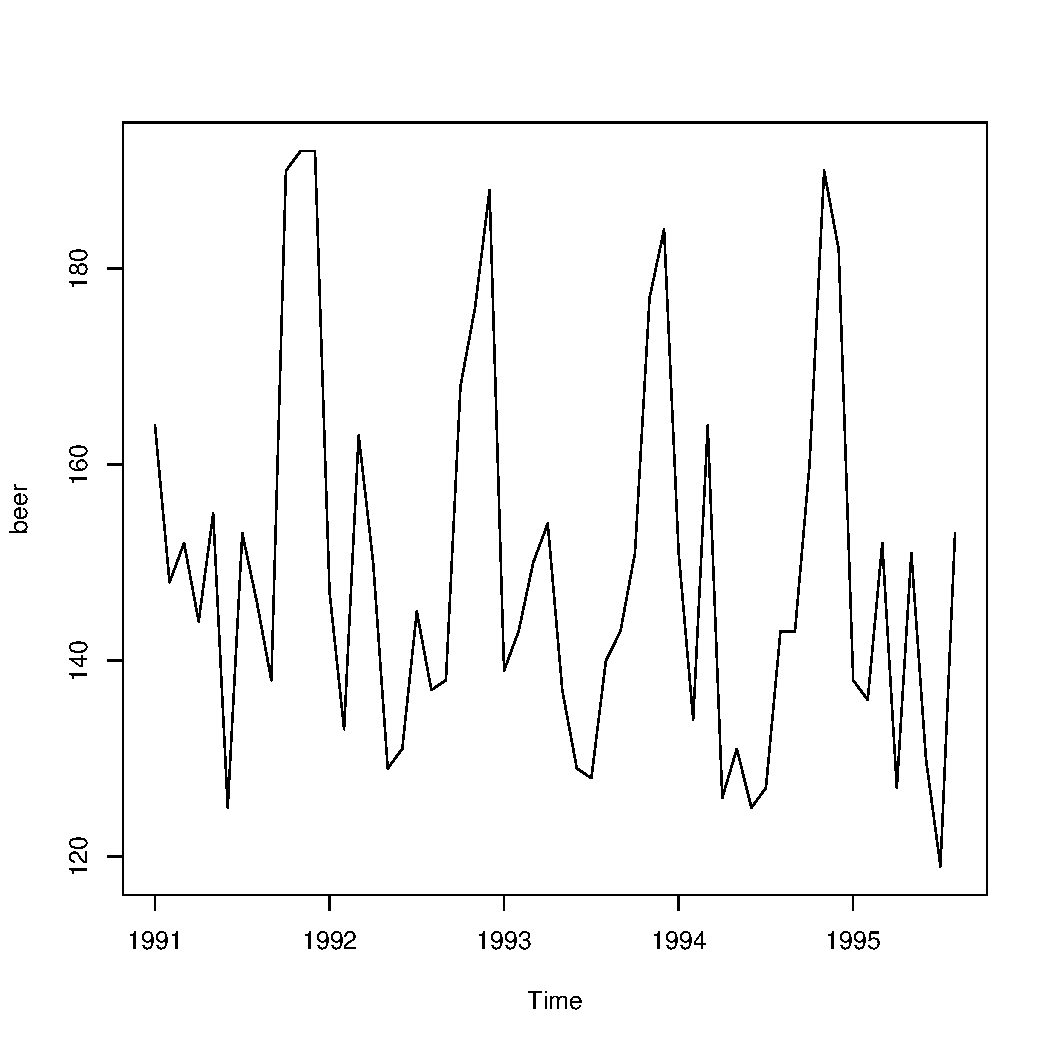
\includegraphics[width=.45\linewidth]{beer}
\label{fig:beer:plot}}
\subfigure[Seasonal plot of the  beer production over a year period.  R> \texttt{seasonplot(beer)}]{
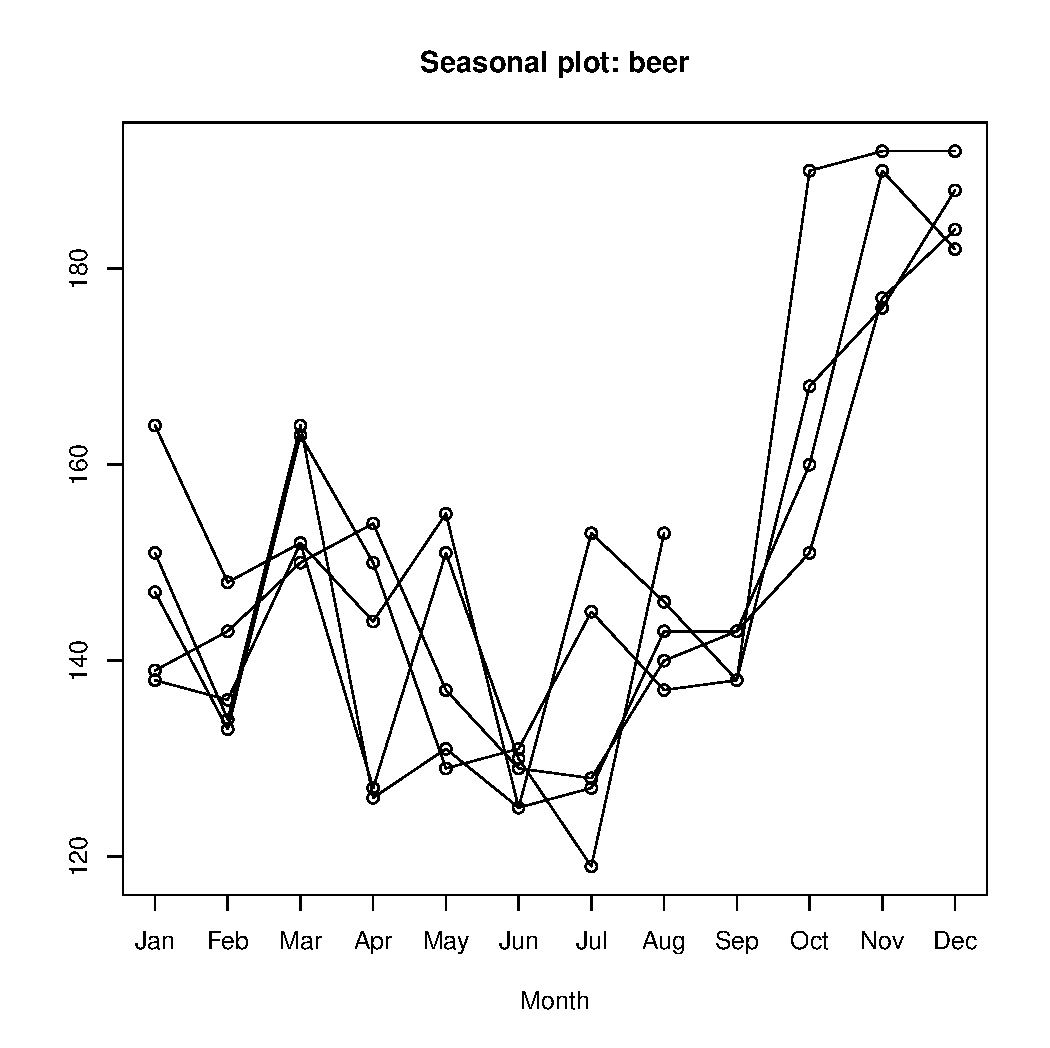
\includegraphics[width=.45\linewidth]{seasonbeer}
\label{fig:season:beer}}
\caption{Monthly Australian beer production (in millions of
 litres).}
\end{figure}

%%
\section{Time Series Patterns}
Time series can be decomposed onto several components:
\begin{enumerate}
\item \textbf{Trend:} a long term increase or decrease occurs.

\item \textbf{Seasonal:} series influenced by seasonal factors. Thus the
series exhibits a behaviour that more or less repeats over a {\it
fixed period of time}, such as a year. Such behaviour is easily
demonstrated in a {\it seasonal plot},
where the data is plotted according to where in the seasonal cycle
it was observed).
\item \textbf{Cyclical (not addressed in this course):} series rises and falls regularly but these are
{\it not of fixed period}. Example: economic data rises and falls
according to the business cycle, but this cycle varies in length
considerably.
\item \textbf{Error:} this corresponds to random fluctuations that cannot be explained by a deterministic pattern.
\end{enumerate}


\paragraph{Exercise.} In the software R, split a time series (e.g. time series \texttt{beer}, \texttt{airpass}, and \texttt{dowjones}) into trend component, seasonality component and noise component, using the function \texttt{decompose}.
  



\paragraph{Exercise.} What patterns do you recognise in the beer data ?

\paragraph{Exercise.} Can you explain the increase of sales of beer at the end of the year ?



\begin{definition}
The {\it AutoCorrelation Function (ACF)} 

For a time series $y_1,y_2,\ldots,y_n$,  the autocorrelation at lag  k is:
$$
r_k =  \frac{\sum_{t=k+1}^n
(y_t - \bar{y})(y_{t-k}-\bar{y})}{\sum_{t=1}^n (y_t - \bar{y})^2},
$$
where $\bar{y}=\frac{1}{n}\sum_{t=1}^n y_t $ is the mean of the series. 
The ACF can be plotted reporting the values $r_k$ on the $y-axis$ with the lag $k$ on the abscissa.

\label{def:ACF}
\end{definition}


\begin{definition}
The {\it Partial AutoCorrelation Function (PACF)} is another useful method to examine serial dependencies. This is an extension of the autocorrelation, where the dependence on the intermediate elements (those within  the lag) is removed. 
The set of partial autocorrelations at different lags is called the
{\it partial autocorrelation function} (PACF) and is plotted like
the ACF. 
\label{def:PACF}
\end{definition}


Figure \ref{fig:tsdisplay:beer} shows time plot, ACF, and PACF for the beer data. 

\begin{figure}[!h]
\begin{center}
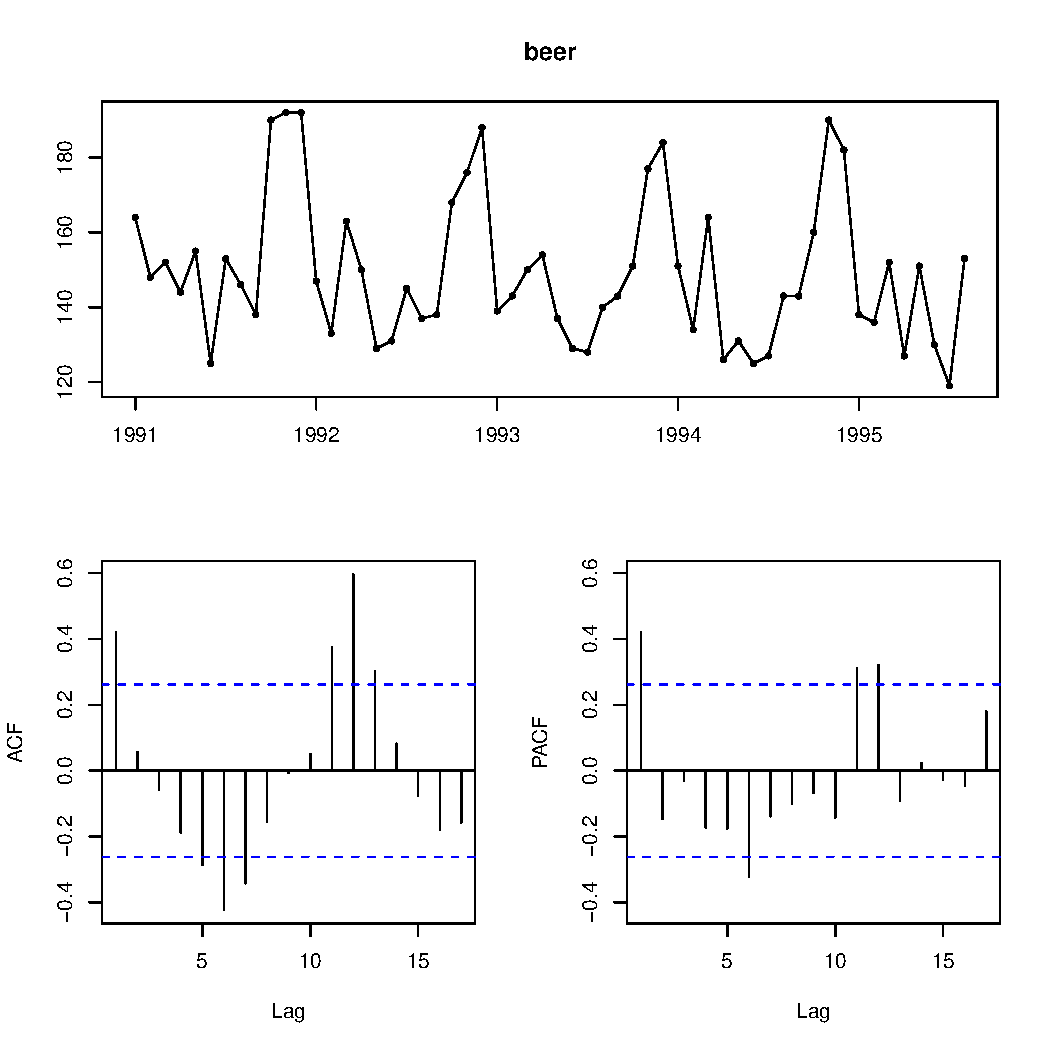
\includegraphics[width=.8\linewidth]{ tsdisplaybeer}
\end{center}
\caption{Displaying the time plot of the beer data with its ACF and PACF plots. R>\texttt{tsdisplay(beer)}}
\label{fig:tsdisplay:beer}
\end{figure}





\section{Additional exercises}


\begin{enumerate}
\item What are the patterns that you see in the time series 1 to 4 in figure \ref{fig:ex:plots}?
\item Identify the ACF functions ABCD given in figure \ref{fig:ex:acf} corresponding to the time plots 1 to 4 in figure \ref{fig:ex:plots}. 
\item Identify the PACF functions  abcd given in figure \ref{fig:ex:pacf} corresponding to the time plots 1 to 4 in figure \ref{fig:ex:plots}. 

\end{enumerate}

\newpage


\begin{figure}[!h]
\begin{tabular}{cc}
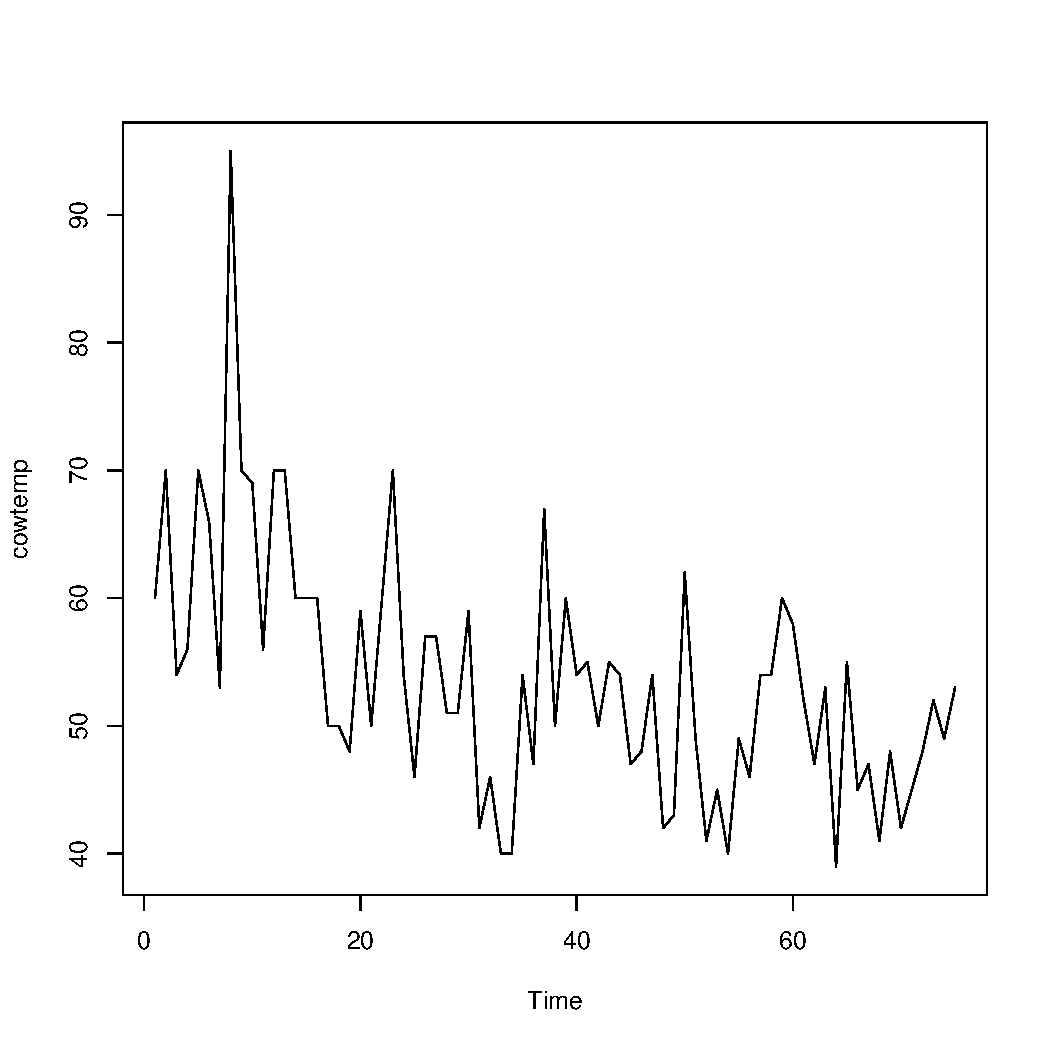
\includegraphics[width=.5\linewidth]{ cowtemp}&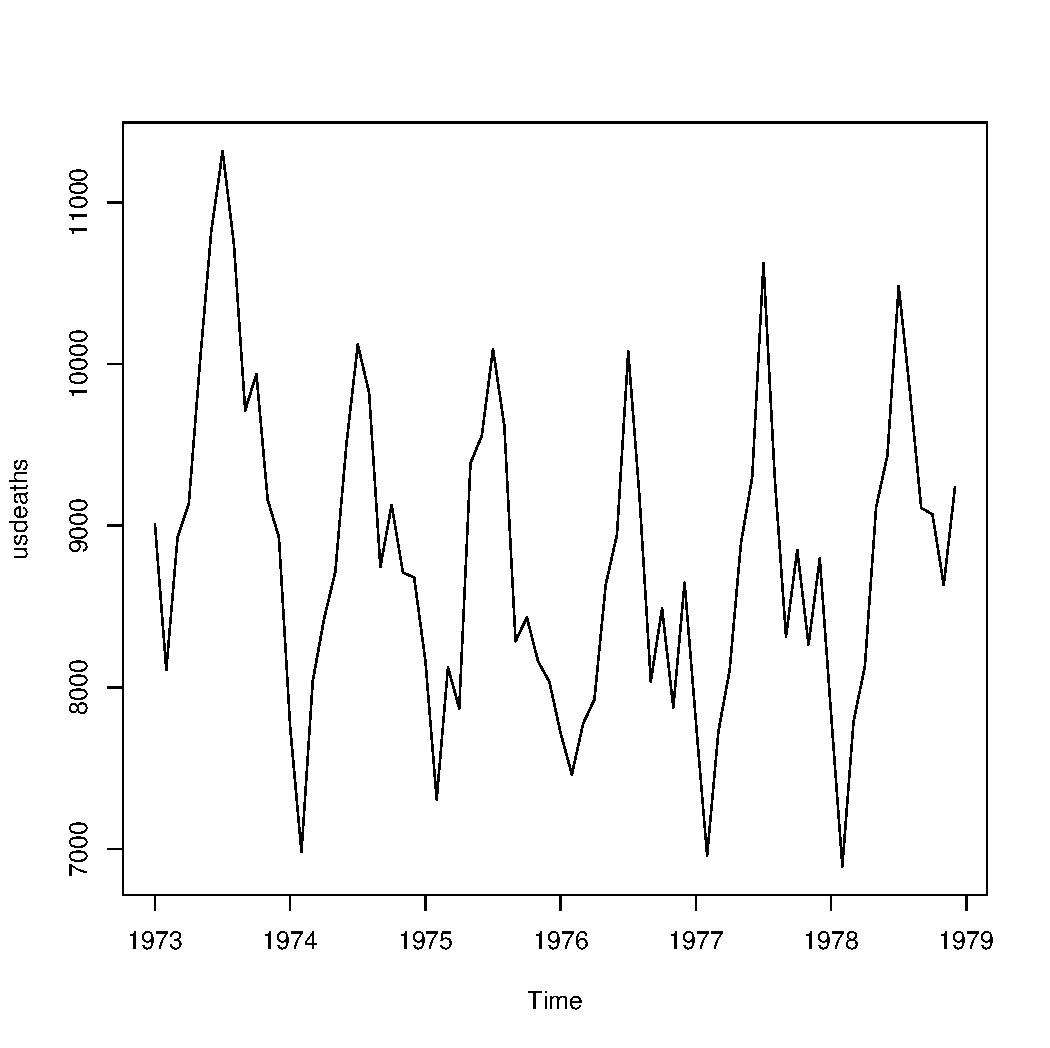
\includegraphics[width=.5\linewidth]{ usdeaths}\\
(1) & (2)\\
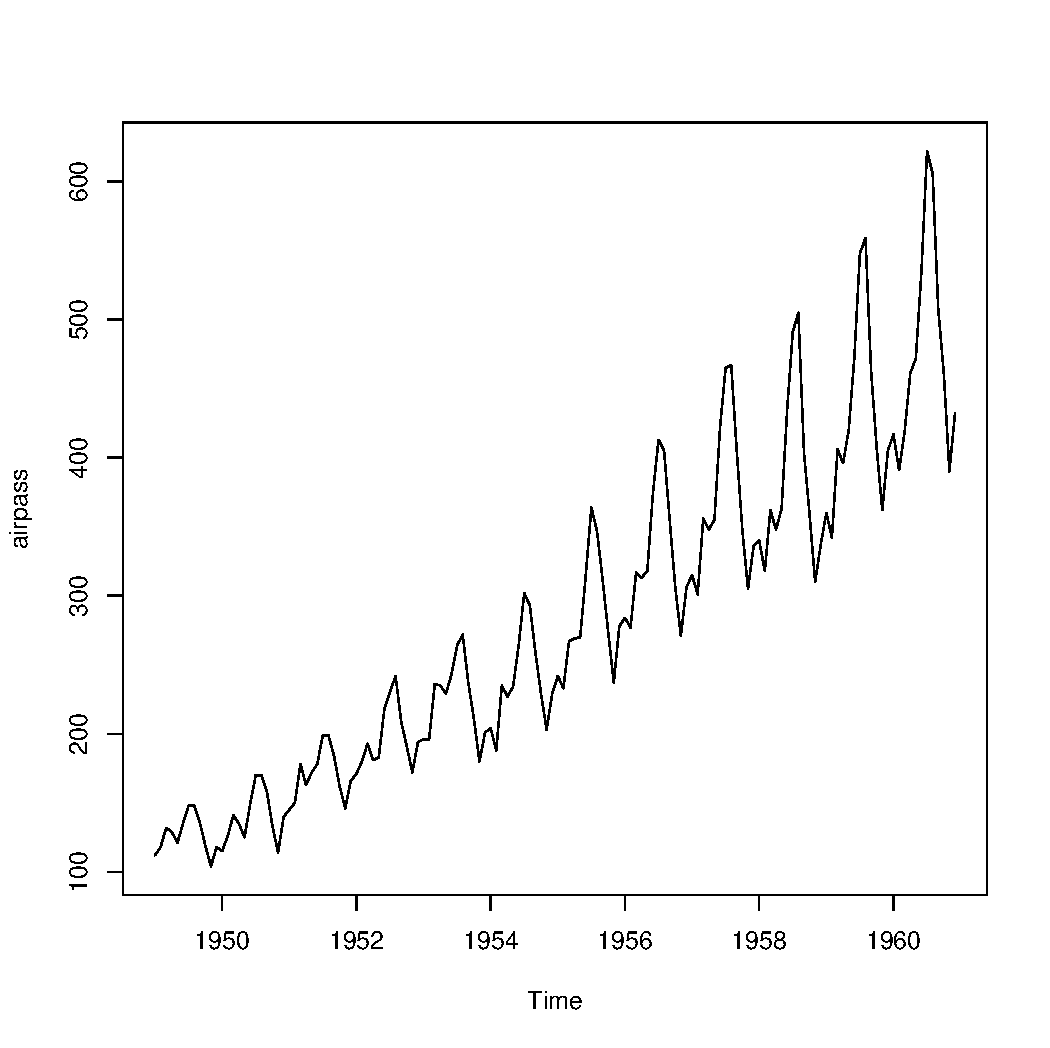
\includegraphics[width=.5\linewidth]{ airpass}&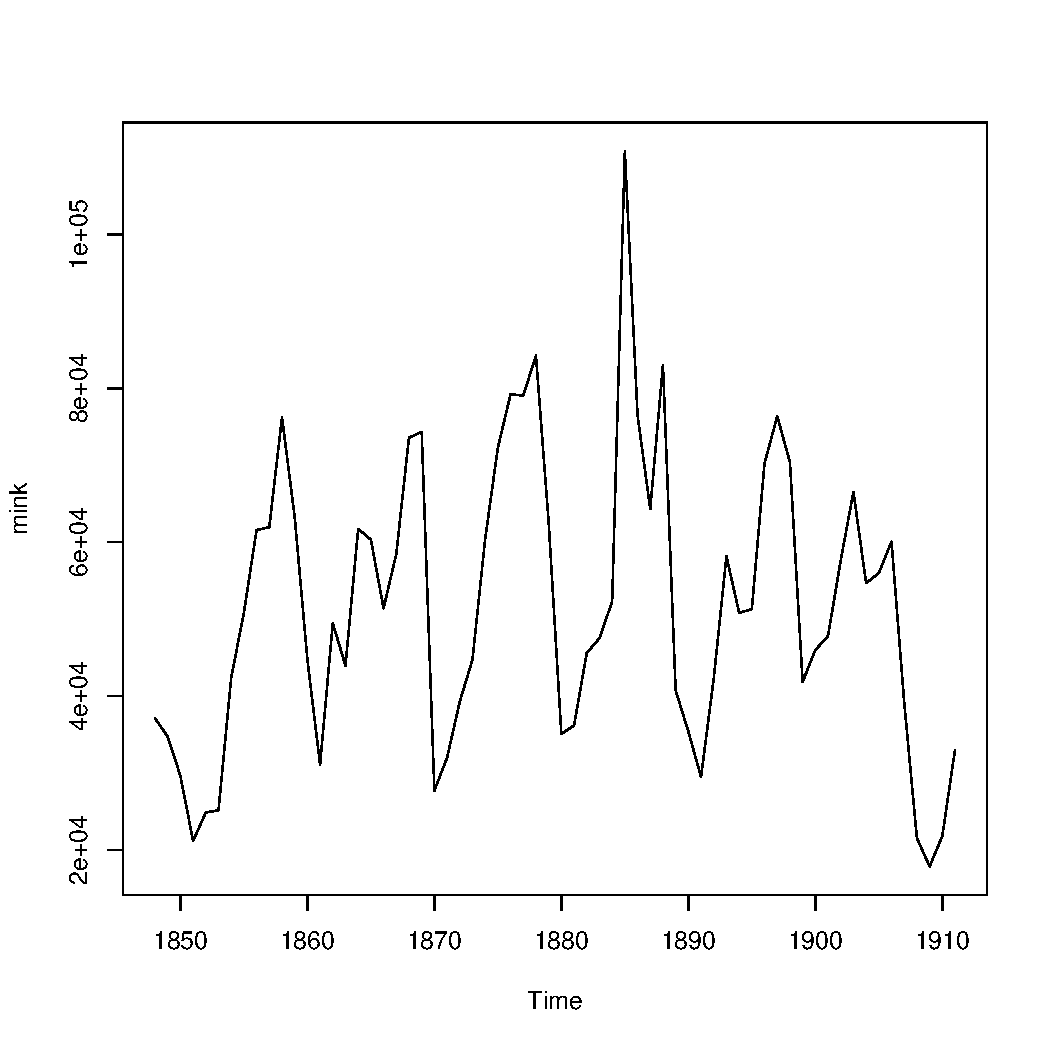
\includegraphics[width=.5\linewidth]{ mink}\\
(3) & (4)\\
\end{tabular}
\caption{Time plots: (1) Daily morning temperature of a cow, (2) Accidental deaths in USA, (3) International airline passengers and (4)  Annual mink trapping.} \label{fig:ex:plots}
\end{figure}

\begin{figure}[!h]
\begin{tabular}{cc}
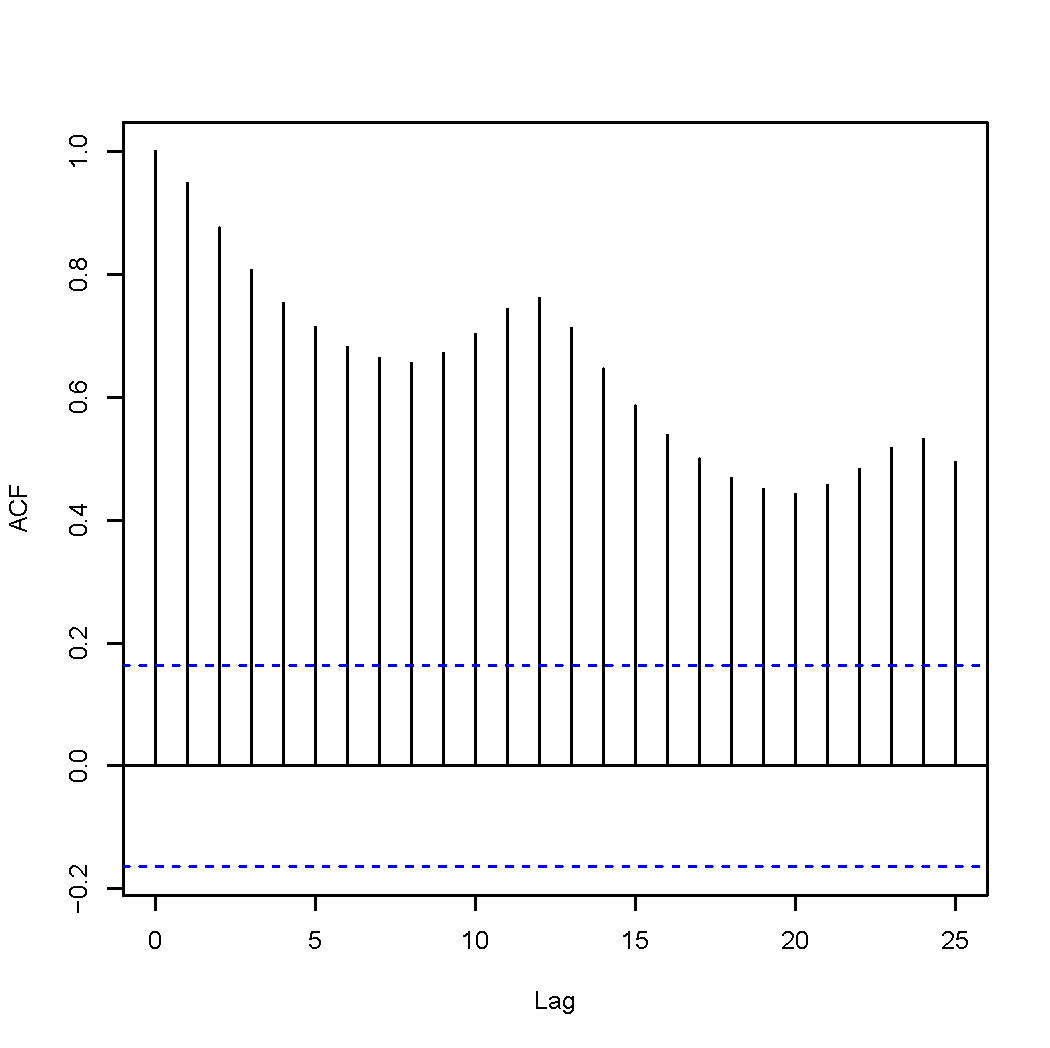
\includegraphics[width=.5\linewidth]{ airpassACF}&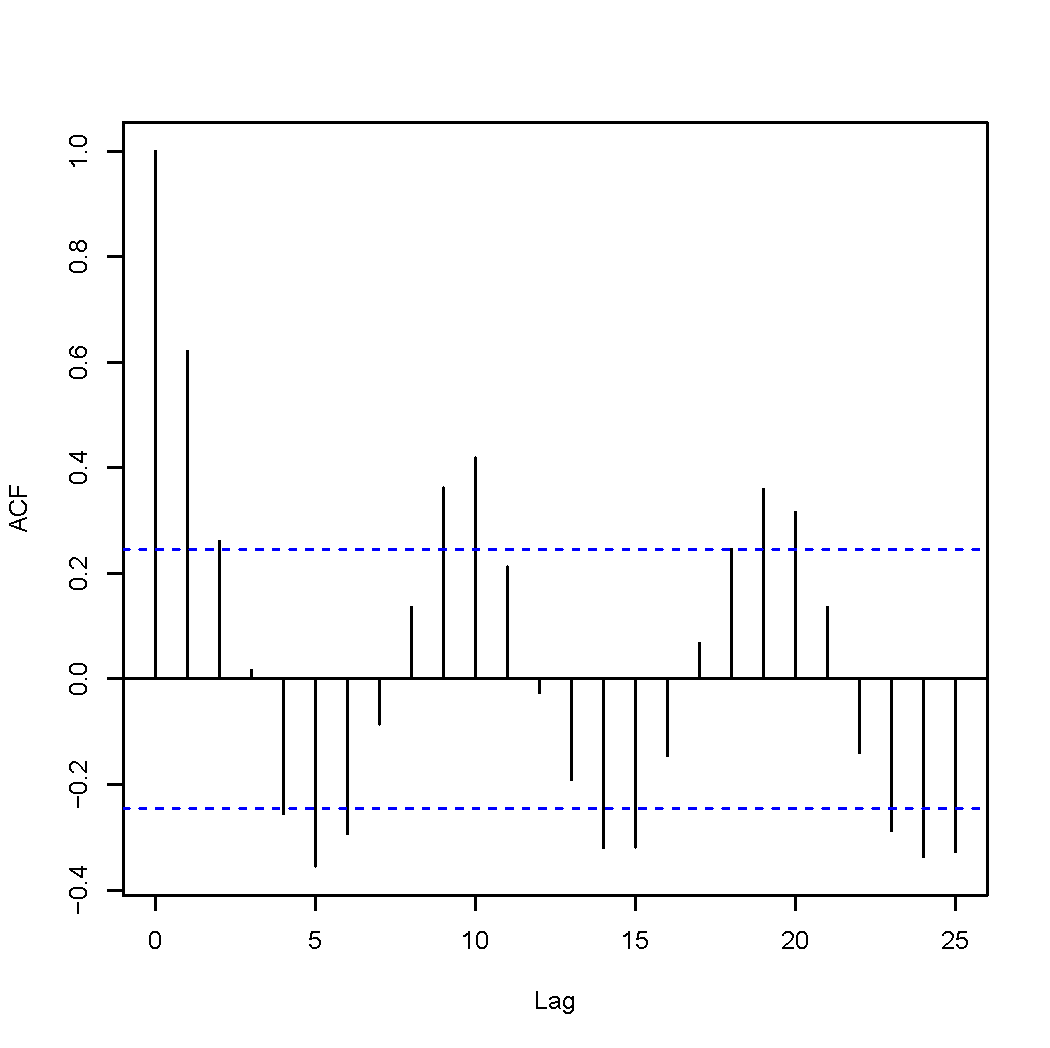
\includegraphics[width=.5\linewidth]{ minkACF}\\
(A)&(B)\\
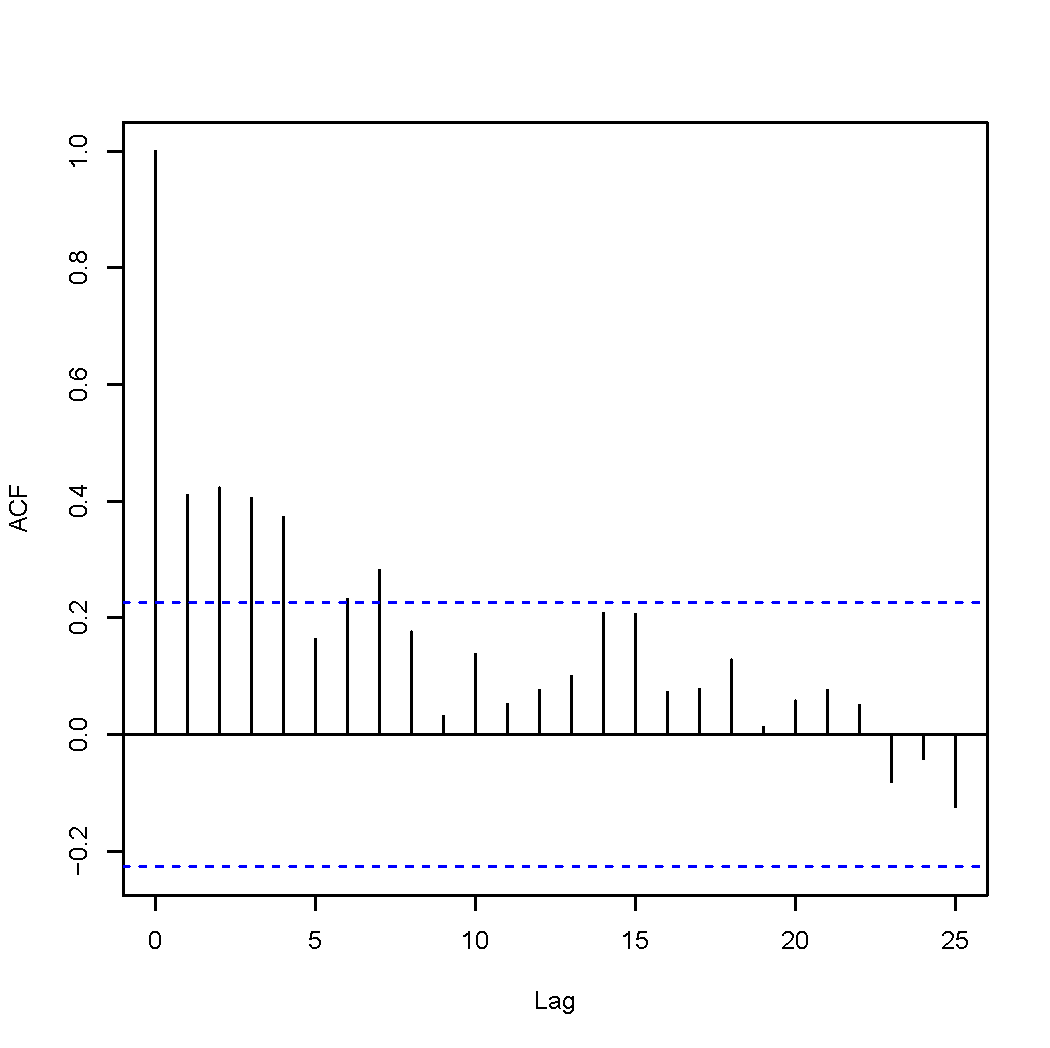
\includegraphics[width=.5\linewidth]{ cowtempACF}&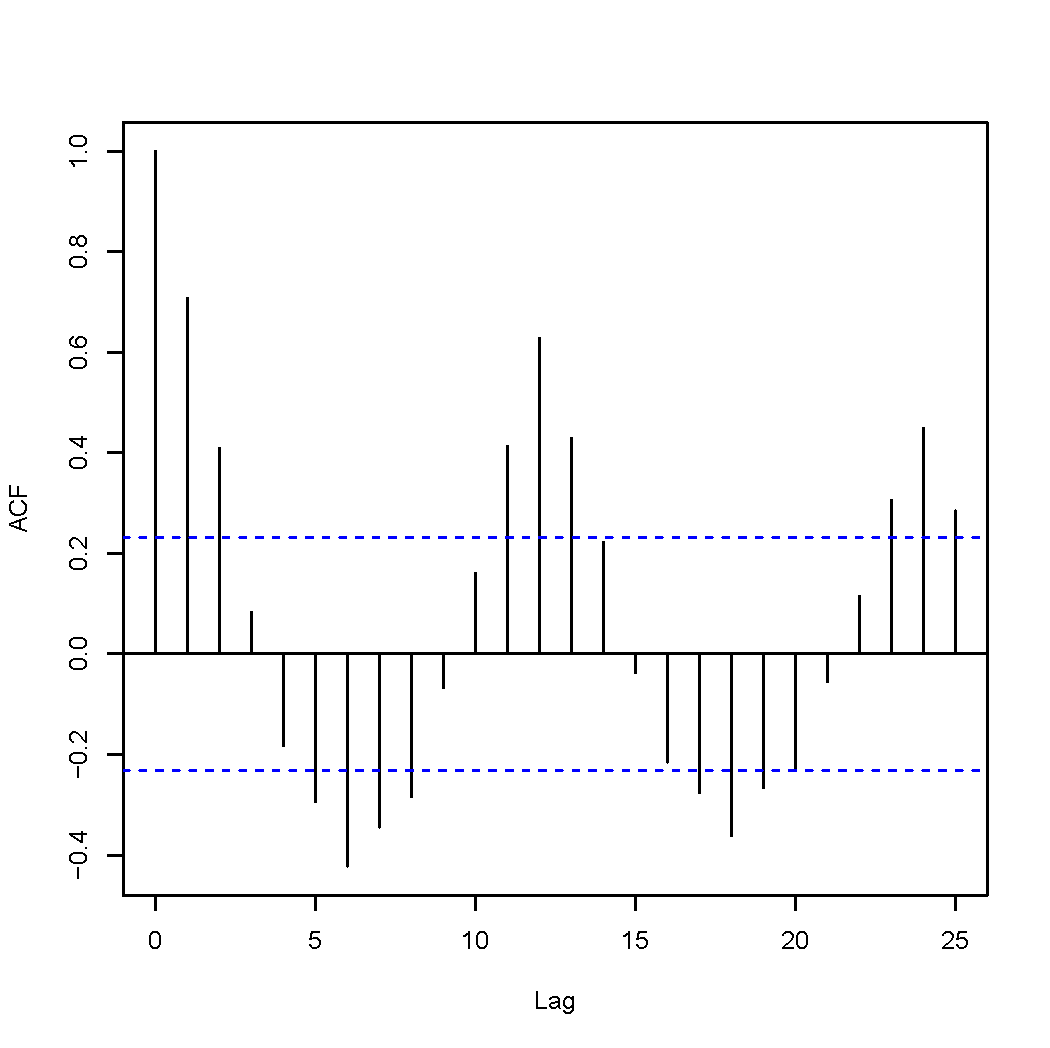
\includegraphics[width=.5\linewidth]{ usdeathsACF}\\\
(C) & (D)\\
\end{tabular}
\caption{ACF. Example of R command for usdeaths time series >\texttt{acf(ts(usdeaths,freq=1),25)}.}\label{fig:ex:acf}
\end{figure}


\begin{figure}[!h]
\begin{tabular}{cc}
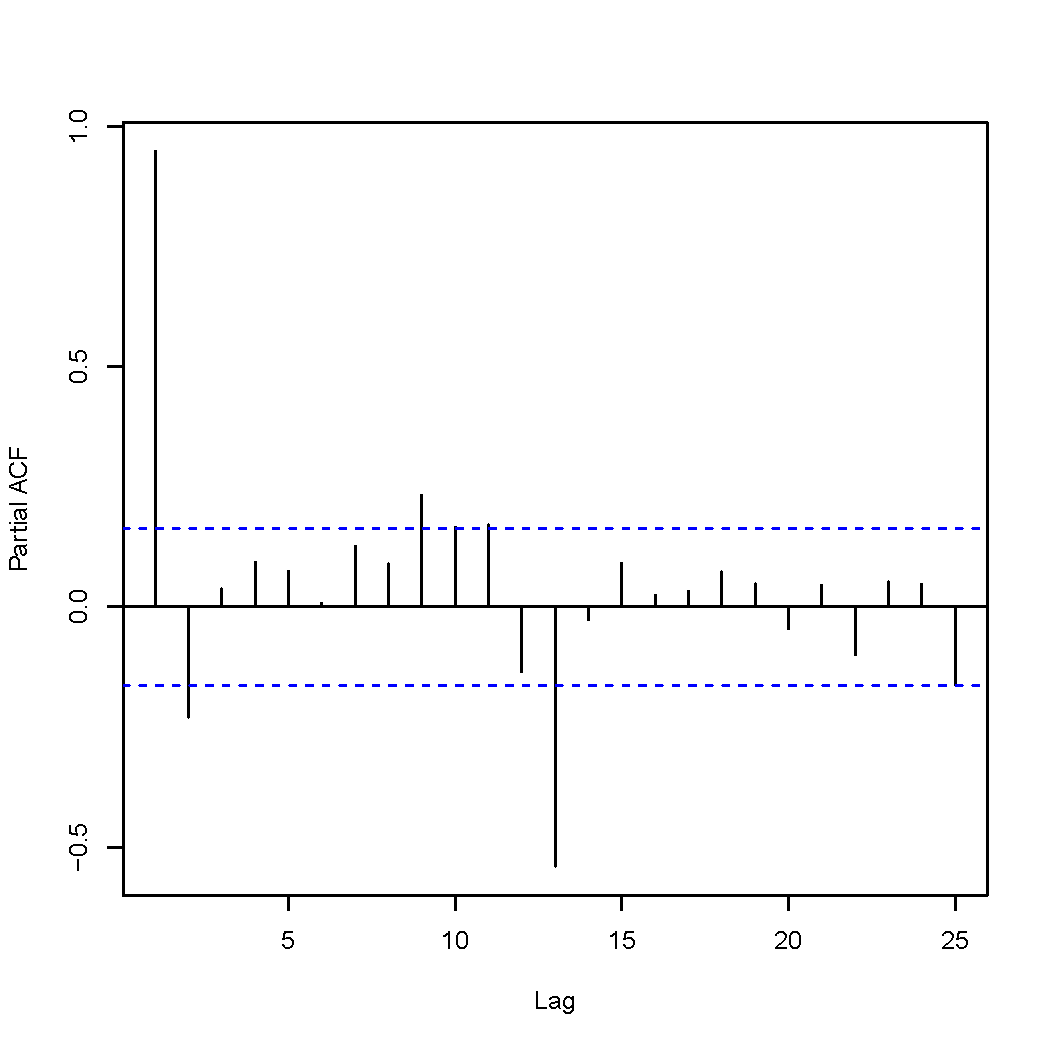
\includegraphics[width=.5\linewidth]{ airpassPACF}&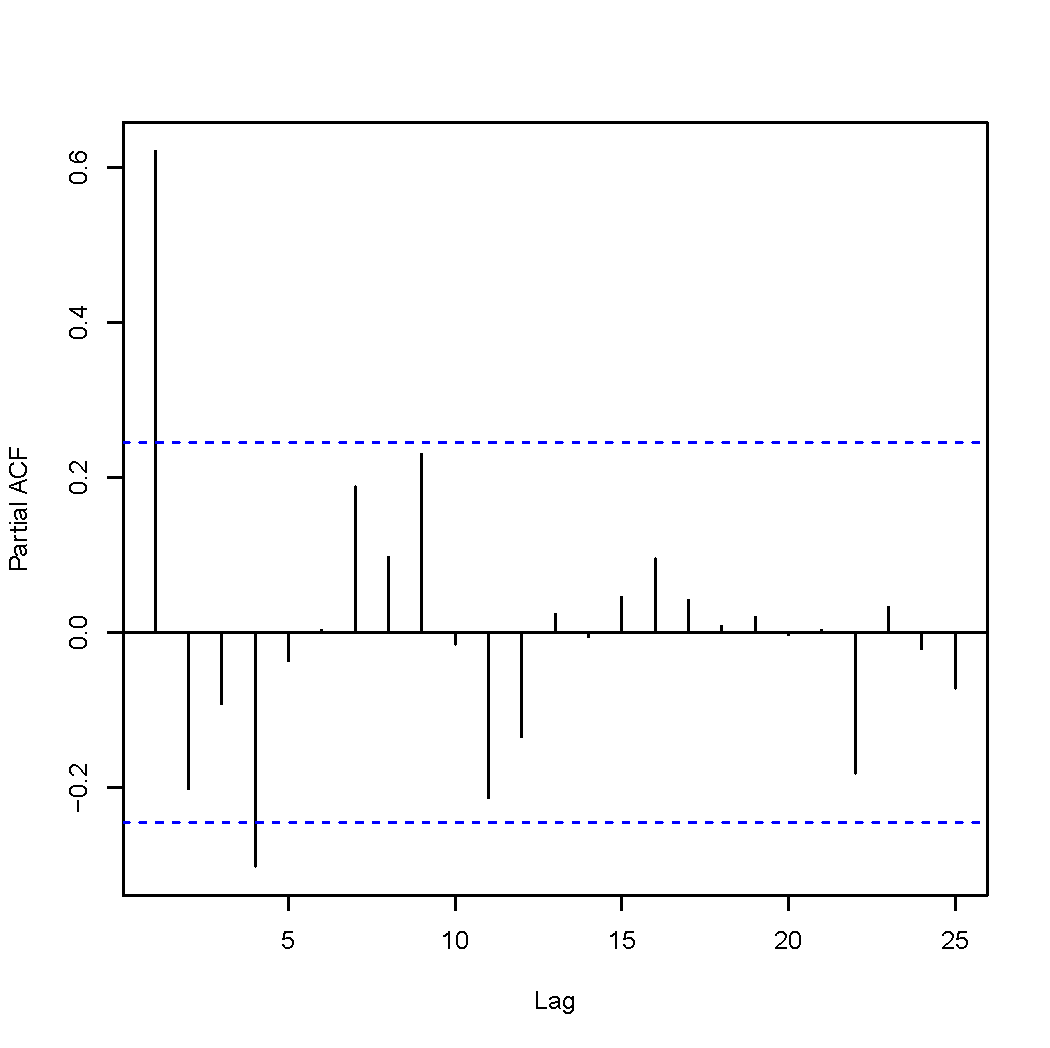
\includegraphics[width=.5\linewidth]{ minkPACF}\\
(a) &(b)\\
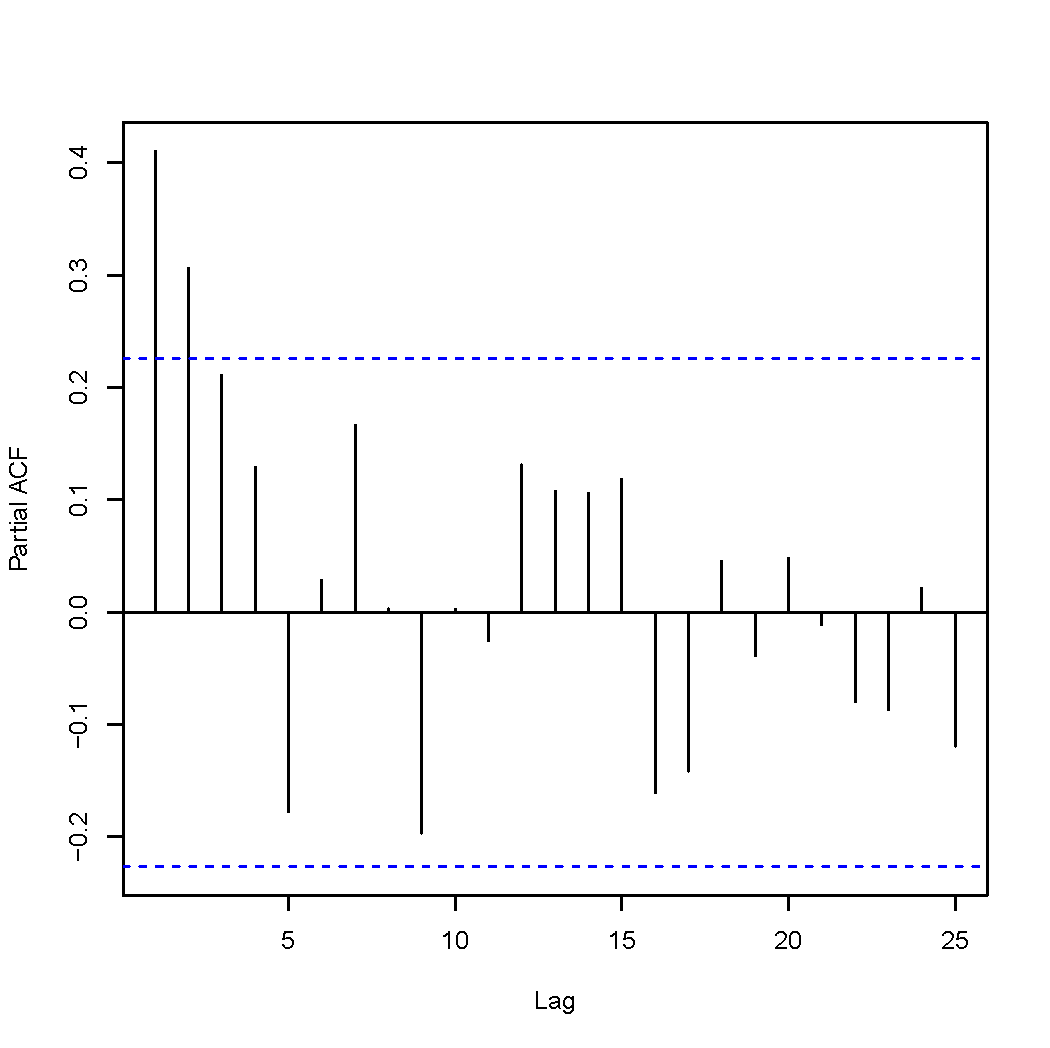
\includegraphics[width=.5\linewidth]{ cowtempPACF}&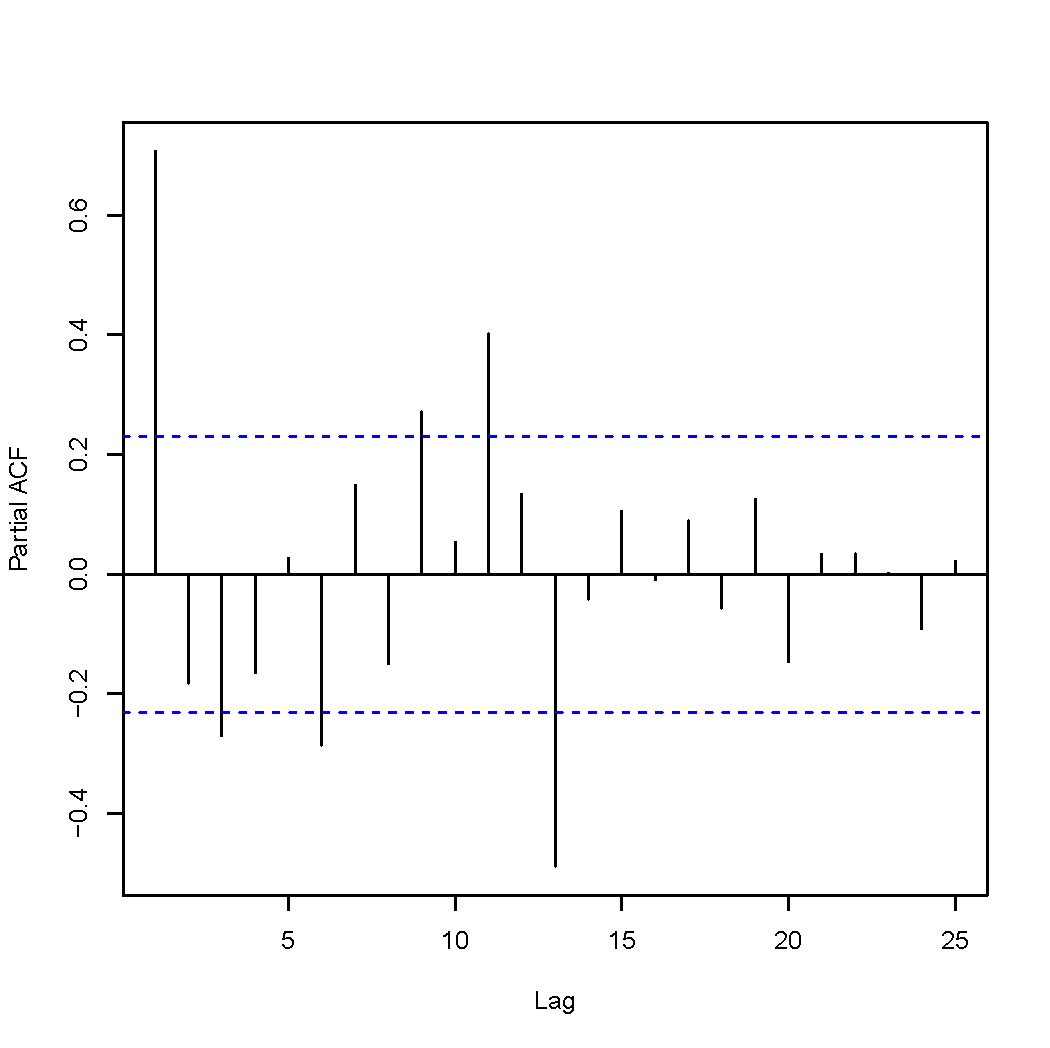
\includegraphics[width=.5\linewidth]{ usdeathsPACF}\\
(c) & (d)\\
\end{tabular}
\caption{PACF. Example of R command for usdeaths time series >\texttt{pacf(ts(usdeaths,freq=1),25)}.} \label{fig:ex:pacf}
\end{figure}







%%%%%%%%%%%%%%%%%%%%%%%%%%
%%%%%%%%%%%%%%%%%%%%%%%%%%
\part{Ad-Hoc Algorithms: Holt-Winters Algorithms } \label{part:Holt:Winters}

This part introduces a number of forecasting methods called Holt-Winters Algorithms which are not explicitly based on a probability models, and can be seen as being of an ad-hoc nature \cite{Chatfield2001}.
Chapter \ref{sec:SES:chp} introduces an algorithm suitable to be fitted to a time series with no or little trend and no seasonal patterns.  
A second algorithm  is introduced  in chapter \ref{sec:des:chp} to deal with time series with trends but no seasonal patterns.
Chapter \ref{sec:hw:chp} proposes two algorithms for dealing with time series  presenting both a trend and a seasonal component.
Chapter \ref{chp:mape:rmse} proposes criteria that can be used to select the 'best algorithm' for a particular time series.
 


%%%%%%%%%%%%%%%%%%%%%

\chapter{Single Exponential Smoothing Algorithm}
\label{sec:SES:chp}



\section{Notations}

From now on in the course we use the following notation:
\begin{itemize}
\item $y_1, y_2, \ldots,y_n$ are the observed values of the time
series
\item $y_n$ is the last value of the series to be observed i.e.\
we are currently at time $n$ (months, quarters, years...)
\item Forecasts for the value of the series at future times $n+1,n+2,\ldots$, using a model fitted to $y_1,\ldots,y_n$, are denoted $F_{n+1}$, $F_{n+2},\ldots$. The
$k$-step ahead forecast from time $n$ would be $F_{n+k}$.
\item Fitted values using the model are $F_1,\ldots,F_n$.
\item The residuals or errors are $y_1 - F_1,\ldots,y_n - F_n$.
\end{itemize}


\subsection{Single Exponential Smoothing}

There is no obvious statistical model that
we try to fit (by regression or another fitting technique). Exponential Smoothing is
simply an algorithm for creating forecasts iteratively on the basis
of how well one did with previous forecasts.


\begin{itemize}
\item Suppose we make a forecast $F_t$ for the value of $y_t$ (which is not yet observed).
\item Now we observe $y_t$ and wish to make a forecast $F_{t+1}$.
We do this by taking our old forecast $F_t$ and adjusting it using
the error in forecasting $y_t$ as follows:
\[ F_{t+1} = F_t + \alpha (y_t - F_t), \]
where $\alpha$ is between 0 and 1.
\item The nearer $\alpha$ is to 1 then the larger the adjustment.
\item We cannot forecast the first term in the series (since $F_1
= F_0 + \alpha (y_0 - F_0)$ and there is no $F_0$ or $y_0$). By
convention, we fix $F_1 = y_1$ and only forecast $y_2$ onwards.
\end{itemize}

\begin{table}[!h]
\begin{center}
\ovalbox{  
$
\begin{array}{l}
\\
\text{Init: } F_1=y_1\quad \text{and choose\ }  0<\alpha<1\\
\text{Forecast:}\\
\quad\left|\begin{array}{l}
F_{t+1}=F_t+\alpha \ (y_t-F_t)
\end{array}\right.\\
\text{Until no more observation}\ \text{are available then}\\
\quad F_{n+k}=F_{n+1},\ \forall k\geq 1\\
\\
\end{array}
$
}
\caption{Simple Exponential Smoothing  (SES) Algorithm.}
 \end{center}
\end{table}




%%%%%%%%%%%%%%%%%%%%%%%%%%%%%%%%%
\section{What does Exponential Smoothing Really Do?} 
If we
recursively apply the smoothing equation to $F_{t+1}$, we get:
\begin{eqnarray*}
F_{t+1} & = & F_t + \alpha\ (y_t - F_t) \\
& = & [F_{t-1}+\alpha\ (y_{t-1} - F_{t-1})] + \alpha\ (y_t -
[F_{t-1}+\alpha\ (y_{t-1} - F_{t-1})]) \\
& = & \alpha\ y_t + \alpha\ (1-\alpha) \ y_{t-1} + (1-\alpha)^2 \ F_{t-1},
\end{eqnarray*}
Now $F_{t+1}$ is in terms of $y_t, y_{t-1}$ and $F_{t-1}$. We can
repeat this, replacing $F_{t-1}$ by $F_{t-2} + \alpha(y_{t-2} -
F_{t-2})$, to get $F_{t+1}$ is in terms of $y_t, y_{t-1}, y_{t-2}$
and $F_{t-2}$. Doing this replacement another $t-3$ times, we end up
with $F_{t+1}$ in terms of $y_1,\ldots,y_t$ and $F_1$, and the
following equation for $F_{t+1}$:
\begin{equation}
 F_{t+1} = \alpha\ y_t + \alpha\ (1-\alpha)\ y_{t-1} + \alpha\
(1-\alpha)^2\ y_{t-2} + \cdots + \alpha\ (1-\alpha)^{t-1}\ y_1 + (1 -
\alpha)^t\  F_1
\label{eq:ses}
\end{equation}
 So {\it exponential smoothing forecasts are a
weighted sum of {\bf all} the previous observations}.





\section{Exercises}

\begin{enumerate}
\item What is $F_{t+1}$ when $\alpha = 0$? What
happens as $\alpha$ increases to 1? What range of values must
$F_{t+1}$ lie in?


\item Here is a short time series. Calculate the
exponentially smoothed series and make a forecast for the next value
in the sequence, using $\alpha = 0.5$ and $\alpha = 0.1$:


\begin{center}
\begin{tabular}{|c|c|cc|cc|}
\multicolumn{1}{|c|}{$t$} & \multicolumn{1}{c|}{$y_t$} &
\multicolumn{1}{p{3cm}}{\hspace{.5cm}$F_t$ (for $\alpha = 0.5$)} &
\multicolumn{1}{p{2cm}|}{\hspace{.6cm}error} &
\multicolumn{1}{p{3cm}}{\hspace{.5cm}$F_t$ (for $\alpha = 0.1$)} &
\multicolumn{1}{p{2cm}|}{\hspace{.6cm}error} \\ \hline
  &       &   &   &   &   \\
1 & 3     & 3 & 0 & 3 & 0 \\
  &       &   &   &   &   \\
2 & 4     &   &   &   &   \\
  &       &   &   &   &   \\
3 & 2     &   &   &   &   \\
  &       &   &   &   &   \\
4 &       &   &   &   & \end{tabular}
\end{center}


\item Can you make $k$-step ahead forecasts using exponential smoothing?
\item Which observation is given the biggest weight in
the formula (\ref{eq:ses}) for $F_{t+1}$. Which is given the smallest? Is this
sensible?
\end{enumerate}






%%%%%%%%%%%
\chapter{Double exponential Smoothing Algorithm} 
\label{sec:des:chp}

Double exponential Smoothing (DES) Algorithm (also known as  Holt's Linear Method) is an extension to the SES algorithm originally designed for time series with no trend nor seasonal patterns.
 It includes  a term to model linear trends. 
Holt's method allows the estimates of level  ($L_t$) and slope ($b_t$) to be adjusted with each new
observation.  

\begin{table}[!h]
\begin{center}
\ovalbox{  
$
\begin{array}{l}
\\
\text{Init: } L_1 = y_1 \quad b_1 = y_2 -
y_1\quad F_1=y_1\quad \text{and choose\ } \\
  0\leq\alpha\leq1\ \text{and}\ 0\leq\beta\leq1\\
\text{Compute and Forecast:}\\
\quad\left|\begin{array}{l}
L_t  =  \alpha \ y_t + (1 - \alpha)\ (L_{t-1} + b_{t-1}) \\
b_t  =  \beta\ (L_t - L_{t-1}) + (1 - \beta)\ b_{t-1}\\
F_{t+1}=L_t+b_t\\
\end{array}\right.\\
\text{Until no more observation}\  \text{are available then}\\
\quad F_{n+k}=L_{n}+k\ b_{n}, \ \forall k\geq 1\\
\\
\end{array}
$
}
\caption{Double Exponential Smoothing (Holt's Linear Model) Algorithm.}
 \end{center}
\end{table}
Note that  no forecasts or fitted values  can be computed until $y_1$ and $y_2$ have been
observed. Also by convention, we let $F_1 = y_1$.


\section{Exercises}

\begin{enumerate}
\item Calculate the level and slope of the series on
the next page by Holt's linear method, using $\alpha = 0.5$ and
$\beta = 0.1$. Compute, at each point, the 1-step ahead forecast
$F_{t+1} = L_t + b_t$.

\begin{center}
\begin{tabular}{|c|c|cc|cc|}
\multicolumn{1}{|c|}{$t$} & \multicolumn{1}{c|}{$y_t$} &
\multicolumn{1}{p{3cm}}{\hspace{1.2cm}$L_t$} &
\multicolumn{1}{p{2cm}|}{\hspace{.6cm}$b_t$} &
\multicolumn{1}{p{3cm}}{\hspace{.5cm}$F_{t} = L_{t-1}+b_{t-1}$} &
\multicolumn{1}{p{2cm}|}{\hspace{.3cm} $y_t - F_t$} \\
\hline
  &       &   &   &   &   \\
1 & 3     & 3 & 1 & 3 & 0 \\
  &       &   &   &   &   \\
2 & 4     &   &   & 4 & 0  \\
  &       &   &   &   &   \\
3 & 2     &   &   &   &   \\
  &       &   &   &   &   \\
4 &       &   &   &   & \end{tabular}
\end{center}



\end{enumerate}



\section{Final comments}

In summary, exponential smoothing is good for forecasting data with
no trend or seasonal patterns. If there is a linear trend, Holt's
method (i.e. D.E.S) can be used. For data with a shift, exponential smoothing is able to adapt to the shift, but the speed at which it does so depends on $\alpha$.


\begin{table}[!h]
\begin{center}
\begin{tabular}{c|ccc}
\hline
\hline
time series patterns:&  & & \\
trend& no & yes & no/yes\\
seasonal &no &no&yes\\
noise & yes & yes &yes\\
\hline
Algorithms & SES & DES  & \\
\hline
parameters& $\alpha$ & $(\alpha,\beta)$ &\\
\hline
\hline
\end{tabular}
\caption{Holt-Winters Algorithms.}
\end{center}
\end{table}



%%%%%%%%%%%%%%%%%%%%%%%%%%%
\chapter{Comparing Holt-Winters Forecasting Algorithms}
\label{chp:mape:rmse}
\begin{itemize}
\item In Single exponential smoothing (SES), how do we pick a value of
$\alpha$?
\item In Holt's Linear Method (DES), how do we pick values of $\alpha$
and $\beta$?
\item When faced with many alternative forecast models, how do we
decide which one to use?
\end{itemize}

\section{Definitions}
Given a time series $y_1,\ldots,y_n$, fit a model and compute the
fitted  values $F_1,\ldots,F_n$.

\begin{definition}[SSE]
The Sum of Square Errors is defined by:
$$
\mathrm{SSE}=\sum_{t=1}^n (y_t-F_t)^2
$$
\end{definition}

In R, the computer selects the best forecasting model by finding the parameters, $\alpha$ for SES or $(\alpha,\beta)$ for DES, such that SSE is minimal.
Other software may use other criteria such as RMSE and MAPE.


\begin{definition}[RMSE]
 The {\it root mean square error} of the
model is:
\[ \mbox{RMSE} = \sqrt{\frac{1}{n} \sum_{t=1}^n (y_t - F_t)^2.}= \sqrt{\frac{\mathrm{SSE}}{n}} \] 
\end{definition}

Note that the same parameters ($\alpha$ or $(\alpha,\beta)$) would be found when minimising the SSE or the RMSE.



\begin{definition}[MAPE]
 The {\it mean absolute percent error} is:
\[ \mbox{MAPE} = 100 \frac{1}{n} \sum_{t=1}^n  \left| \frac{y_t - F_t}{y_t} \right|. \]
It is written as a percentage. Again, pick the model with the
smallest MAPE.
\end{definition}

Other software may use MAPE for finding the best parameters. This would  give slightly different estimates of the parameters than using the SSE/RMSE.

\section{Exercises}

\begin{enumerate}
 \item Here is a short time series and its
exponentially smoothed forecast with $\alpha = 0.5$. Compute the
error and then the RMSE and MAPE:

\begin{center}
\begin{tabular}{ccccc}
$y_i$ & $F_i$ & $y_i - F_i$ & $(y_i - F_i)^2$ & $\left| \frac{y_i - F_i}{y_i} \right|$ \\ \hline 4 & 4 &  \\
3 & 4 &   \\
5 & 3.5 &  \\
7 & 4.25 &  \\
5 & 5.73 &  \\
6 & 5.26 &  \\
4 & 5.73 & \\ \hline
\end{tabular}
\end{center}

\end{enumerate}

%%%%%%%%%%%%%%%%%%%%%%%%%%%
\chapter{Holt-Winters' Exponential Smoothing with Seasonality}
\label{sec:hw:chp}


What about an exponential smoothing for data with a trend and
seasonal behaviour? Winters generalised Holt's linear method to
come up with such a technique, now called Holt Winters. A seasonal
equation is added to Holt's linear method equations. It is done in two ways, additive (cf. table \ref{tab:SHW+}) and multiplicative (cf. table \ref{tab:SHWx}). 


\vspace{.3cm}
\begin{table}[!h]
\begin{center}
\ovalbox{  
$
\begin{array}{l}
\\
\text{Init: } \\
\left|
\begin{array}{l}
L_s  =  \frac{1}{s} \sum_{i=1}^s y_i \\
b_s  =  \frac{1}{s} \left[ \frac{y_{s+1}-y_1}{s} + \frac{y_{s+2}-y_2}{s} +
\cdots + \frac{y_{2s}-y_s}{s} \right]\\
S_i  =  y_i - L_s, \; i=1,\ldots,s\\
\end{array}\right. \\
\text{and choose\ } 0\leq\alpha\leq 1\ \text{and}\ 0\leq\beta\leq 1\ \text{and}\ 0\leq\gamma\leq 1\\
\text{Compute for } t>s :\\
\quad\left|\begin{array}{ll}
\text{\tiny{level} } & L_{t} =\alpha\ (y_{t}-S_{t-s})+(1-\alpha )\ (L_{t-1}+b_{t-1}) \\
\text{\tiny{trend} } & b_{t} =\beta\ (L_{t}-L_{t-1})+(1-\beta )\ b_{t-1}, \\
\text{\tiny{seasonal} } & S_{t} =\gamma\ (y_{t}-L_{t})+(1-\gamma )\ S_{t-s} \\
\text{\tiny{forecast}} & F_{t+1} =L_{t}+ b_{t}+S_{t+1-s} \\
\end{array}\right.\\
\text{Until no more observation} \text{are available}\\
\text{and subsequent forecasts: } \\
F_{n+k} =L_{n}+k\ b_{n}+S_{n+k-s}  \\
\end{array}
$
}
\caption{Seasonal Holt Winter's Additive Model Algorithm (noted SHW$+$).}\label{tab:SHW+}
 \end{center}
\end{table}


\vspace{.3cm}
\begin{table}[!h]
\begin{center}
\ovalbox{  
$
\begin{array}{l}
\\
\text{Init: } \\
\left|
\begin{array}{l}
L_s  =  \frac{1}{s} \sum_{i=1}^s y_i \\
b_s  =  \frac{1}{s} \left[ \frac{y_{s+1}-y_1}{s} + \frac{y_{s+2}-y_2}{s} +
\cdots + \frac{y_{2s}-y_s}{s} \right]\\
S_i  =  \frac{y_i}{L_s}, \; i=1,\ldots,s\\
\end{array}\right. \\
\text{and choose\ }  0\leq\alpha\leq 1\ \text{and}\ 0\leq\beta\leq 1\ \text{and}\ 0\leq\gamma\leq 1\\
\text{Compute for } t>s :\\
\quad\left|\begin{array}{ll}
\text{level } &L_{t} =\alpha\ \frac{y_{t}}{S_{t-s}}+(1-\alpha)\ (L_{t-1}+b_{t-1}) \\
\text{trend } & b_{t} =\beta\ (L_{t}-L_{t-1})+(1-\beta )\ b_{t-1}, \\
\text{seasonal } & S_{t} =\gamma\ \frac{y_{t}}{L_{t}}+(1-\gamma )\ S_{t-s} \\
\text{forecast } & F_{t+1} =(L_{t}+ b_{t})\ S_{t+1-s} \\
\end{array}\right.\\
\text{Until no more observation are available}\\
\text{and subsequent forecasts: }\\
 F_{n+k} =(L_{n}+k\cdot b_{n})\ S_{n+k-s}  \\
\end{array}
$
}
\caption{Seasonal Holt Winter's Multiplicative Model Algorithm (noted SHW$\times$).}\label{tab:SHWx}
 \end{center}
\end{table}


$s$ is the length of the seasonal cycle.
We have to pick the values of $\alpha$, $\beta$ and $\gamma$. As
with the other methods (i.e. SES and DES), we can use the SSE/RMSE\ or MAPE to choose the
best values.



\section{Exercise}

In the table on the next page are the first 14 months beer
production data. \ Since the data have a 12 month seasonal cycle,
we initialise $L_{12}$, $b_{12}$ and $S_1,\ldots,S_{12}$. Use the
additive model formulae to calculate month 13 and 14's level,
trend and seasonality, and make a 1-step ahead forecast for months
13, 14 and 15. Use $\alpha=0.5, \beta=0.3$ and $\gamma=0.9$.

\begin{center}

\begin{tabular}{|cc|p{3cm}p{3cm}p{3cm}|c|} \hline

Month No. & Production & Level $L_t$ & Trend $b_t$ & Seasonal
$S_t$ & Forecast $F_t$ \\

& & & & & \\ \hline

1 & 164 & -- & -- &  5.75 & -- \\

2 & 148 & -- & -- &  $-$10.25 & -- \\

3 & 152 & -- & -- &  $-$6.25 & -- \\

4 & 144 & -- & -- &  $-$14.25 & -- \\

5 & 155 & -- & -- &  $-$3.25 & -- \\

6 & 125 & -- & -- &  $-$33.25 & -- \\

7 & 153 & -- & -- &  $-$5.25 & -- \\

8 & 148 & -- & -- &  $-$12.25 & -- \\

9 & 138 & -- & -- & $-$20.25 & -- \\

10 & 190 & -- & -- & 31.75 & -- \\

11 & 192 & -- & -- & 33.75 & -- \\

12 & 192 & 158.25 & $-$0.65 & 33.75 & -- \\

& & & & & \\ \hline

& & & & & \\

13 & 147 & & & & \\

& & & & & \\

& & & & & \\

14 & 133 & & & & \\

& & & & & \\

& & & & & \\

15 & 163 & & & & \\

& & & & & \\

& & & & & \\ \hline

\end{tabular}

\end{center}

\section{Selecting the best Holt-Winters algorithms}

For a time series, you select the Holt Winters algorithms with the smallest SSE or RMSE or MAPE 
as defined in chapter \ref{chp:mape:rmse}.
To analyse a time series, identify the patterns that occur  in the time series (is there a trend? is there seasonality? there is always noise!), and decide which algorithm(s) is the best suited i.e.
when no seasonality select the best algorithm  between SES and DES, and when there is seasonality, select the best algorithm between SHW+ and SHWx. 
To know more about Holt-Winters algorithms (in particular their limitations),  read at Goodwin short paper   \cite{RePEc:for:ijafaa:y:2010:i:19:p:30-33}. 


%%%%%%%%%%%%%%%%%%%%%%%%%
%%%%%%%%%%%%%%%%%%%%%%%%%


\clearpage
\part{Statistical models: ARIMA}\label{part:ARIMA}

This part is investigating one important class of linear statistical models called ARIMA.
ARIMA models use the same hypotheses and the same approach  as Linear   regression, 
so chapter \ref{chp:LR} (re-)introduces Linear regression and show how Linear regression could be used for Forecasting.
Linear regression however requires the definition of explanatory variables, and the selection of informative explanatory variables can often only be done by domain experts.
In addition to choosing  these explanatory variables, one also needs to collect this data along with the time series of interest.
 On the contrary,  ARIMA models only requires the times series to be recorded for a while, and no additional information is required for analysis.

\vspace{1cm}
\noindent In this part of the lecturenotes:
\begin{itemize} 
\item chapter \ref{chp:AR} introduces AutoRegressive models. The acronym used for these models is AR and corresponds to the first 2 letters of the acronym ARIMA.  
\item chapter \ref{chp:MA} introduces Moving Average models. The acronym used for these models is MA and corresponds to the last 2 letters of the acronym ARIMA. 
\item chapter \ref{chp:ACF:PACF:AR:MA} presents the ACF and PACF in more details, and illustrates what sort of shapes these should have when dealing with time series following perfectly  a AR or MA modelling.
\item chapter \ref{chp:backshift} introduces the backshift operator. This operator is meant to simplifies the mathematical notations for ARIMA models. 
\item To analyse a time series, several ARIMA models can be suitable, and chapter \ref{chp:AIC:BIC} presents two criteria that can be used to select which model is the best to analyse the time series.
\item AR, MA and ARMA models  are not able to deal with time series with a slope, and  chapter \ref{chp:ARIMA} presents how this limitation is overcome by the Integration of differencing.
The I of integration corresponds to the I of the acronym ARIMA: AutoRegressive Integrated Moving Average models.  
\item Seasonal ARIMA models are then introduced in chapter \ref{chp:Seasonal:ARIMA} to model seasonal patterns.


\item Chapter \ref{chp:PreparationTS} presents techniques that can be used to transform a time series such that they become suitable for analysis with ARIMA models.

\end{itemize}

%%%%%%%%%%%%%%%%%%%%%%%%%%%%%%%%%%%%%
\chapter{Linear Regression} \label{chap:linear:regression}
\label{chp:LR}

\section{Regression with one explanatory variable} 


We have collected the data
$(x_1,y_1),(x_2,y_2),\ldots,(x_n,y_n)$, where the $x_i$ are known
{\it predictor} values set by the experimenter and $y_i$ is the
observed {\it response}. We wish to model $y$ as a function of $x$.
In simple linear regression we assume that $y$ is related to $x$ by:
\[ y_i = a + b\  x_i + \epsilon_i, \]
with the assumptions that 
\begin{itemize}
\item $\epsilon_i$ is the error and is normally distributed with
mean 0 and unknown variance $\sigma^2$.
\item $\epsilon_i$ and $\epsilon_j$ are independent when $i\neq j$.
\end{itemize}
 Thus we say that the $y_i$
follow a ``pattern'' $a + b\ x_i$ but with some random,
unpredictable behaviour modelled as a normal distribution. Or, in
other words, given $a$ and $b$, $y_i$ will be normally
distributed with a mean $a + b \ x_i$ and variance
$\sigma^2$.

\begin{enumerate}
\item {\bf Fitting the Model:} The best fitting values of $\alpha$ and
$\beta$ are the {\it least squares estimates} that minimise the Residual Sum of
Squares: 
$$
RSS =\sum_{i=1}^n (y_i - a - b x_i)^2
$$ 
also known as the Sum of Square Errors (SSE).
 The estimates $(\hat{a},\hat{b})$ are then computed such that:
$$
\frac{\partial RSS}{\partial a} =0 \quad \text{and} \quad
\frac{\partial RSS}{\partial b} =0  
$$
giving the \textbf{least squares} estimates:
\begin{equation}
 \hat{b} = \frac{\sum_{i=1}^n (x_i - \bar{x})(y_i - \bar{y})}{\sum_{i=1}^n (x_i - \bar{x})^2}, \;\;\;\;
\hat{a} = \bar{y} - \hat{\beta} \bar{x},
\label{eq:LS0}
\end{equation}
and $\sigma^2$ is
estimated from the sum of squares by the quantity: 
$$
s^2 =\frac{\widehat{RSS}}{(n-2)}
$$
$\widehat{RSS}$ indicates that the RSS value is computed with the least squares estimate $(\hat{a},\hat{b})$.
The denominator $n-2$ corresponds to the degree of freedom in the errors $\lbrace \epsilon_i\rbrace_{i=1,\cdots,n}$: the estimation of 2 parameters 
$(a,b)$ removes 2 degrees of freedom.



The means of $x$ and $y$ are simply estimated by:
$$
\bar{x}=\frac{1}{n}\sum_{i=1}^n x_i \quad \text{and} \quad \bar{y}=\frac{1}{n}\sum_{i=1}^n y_i 
$$

\item {\bf Measuring the Strength of the Linear Relationship:} 
\begin{definition}[correlation coefficient]

Usually we calculate the {\it correlation coefficient}:
\[ r_{xy} = \frac{\sum_{i=1}^n (x_i - \bar{x})(y_i -
\bar{y})}{\sqrt{\left( \sum_{i=1}^n (x_i - \bar{x})^2 \right) \left(
\sum_{i=1}^n (y_i - \bar{y})^2 \right)}}. \] 
\end{definition}

If you note $\mathbf{\tilde{x}}$ a column vector gathering all the values $(x_1-\bar{x},x_2-\bar{x}, \cdots,x_n-\bar{x})$, and $\mathbf{\tilde{y}}$ a column vector collecting all the values $(y_1-\bar{y},y_2-\bar{y},\cdots,y_n-\bar{y})$ then the correlation coefficient corresponds to:
$$ 
r_{xy} =\frac{<\mathbf{\tilde{x}},\mathbf{\tilde{y}}>}{\|\mathbf{\tilde{x}}\|\ \|\mathbf{\tilde{y}}\|}
$$
where $<\mathbf{\tilde{x}},\mathbf{\tilde{y}}>$ is the dot product between  $\mathbf{\tilde{x}}$ and $\mathbf{\tilde{y}}$. $\|\mathbf{\tilde{x}}\|$ (resp. $\|\mathbf{\tilde{y}}\|$) is the norm of the vector $\mathbf{\tilde{x}}$ (resp. $\mathbf{\tilde{y}}$). By definition of the dot product, we have:
$$
<\mathbf{\tilde{x}},\mathbf{\tilde{y}}> =\|\mathbf{\tilde{x}}\|\cdot\|\mathbf{\tilde{y}}\|  \ \cos( \alpha )
$$
where $\alpha$ is the angle between vectors  $\mathbf{\tilde{x}}$  and $\mathbf{\tilde{y}}$. The correlation coefficient is then simplified to $r_{xy} =\cos\alpha$ and consequently has values between $-1$ (perfect negative correlation) and $+1$ (perfect positive correlation). 


\vspace{.5cm}

Another important measure when we do regression is the coefficient of determination.

\begin{definition}[coefficient of determination]

The {\it coefficient of determination} is the correlation between the $y_i$ and
their predicted values from the fitted model $\hat{y}_i =
\hat{a} + \hat{b} x_i$:
\[ R^2 = r^2_{y \hat{y}} = \frac{\sum_{i=1}^n (\hat{y}_i -
\bar{y})^2}{\sum_{i=1}^n(y_i - \bar{y})^2}. \] 
\end{definition}
For simple linear
regression, as explained here, $R^2 = r^2_{xy}$. This is not true
for more general multivariate regression.

\item {\bf Evaluating Model Fit:} We look at the {\it residuals}. These
are the difference between the observed and predicted values for
$y$:
\[ \epsilon_i = y_i - \hat{y}_i.
\]  There are two problems with model fit
that can arise: 
\begin{enumerate} 
\item We have not fit the pattern
of the data.  Any unmodelled relationships between $x$ and $y$
appear in the residuals. A scatter plot of the residuals against the
$x_i$ should show up any unmodelled patterns. 
\item The normally
distributed error assumption is not correct. The residuals should be
independent and normally distributed with variance $\sigma^2$. A
histogram of the residuals can usually verify this.
\end{enumerate}

\item {\bf Outliers:} An observation that has an unusually large
residual is an {\it outlier}. An outlier is an observation that
has been predicted very badly by the model. {\it Standardised
residuals} give a good indication as to whether an observation is
an outlier. We should investigate if there is some special reason
for the outlier occurring. Outliers can also cause problems
because they can significantly alter the model fit, making it fit
the rest of the data worse than it would otherwise.

\item {\bf Making Predictions:} Given a new value $X$, $y$ should be
normally distributed with mean $a + b\  X$ and variance
$\sigma^2$. We replace $a$, $b$ and $\sigma^2$ by their
estimates and so forecast the value of $y$ to be $\hat{y} =
\hat{a} + \hat{b}X$. A 95\% prediction interval turns out
to be:
$$
\hat{a} + \hat{b}X \pm 2 \ s \
$$

\item {\bf Statistical Tests in Regression:} An {\it F-test} is used to
 determine if there is any significant linear relationship between
 $x$ and $y$. In other word, it is checking if the hypothesis $b=0$ is true or not.  The test statistic is:
 \[ F = \frac{\sum_{i=1}^n (\hat{y}_i - \bar{y})^2}{\left(
 \sum_{i=1}^n (y_i - \hat{y}_i)^2 \right) / (n-2)}, \]
 which is compared with the F-value having 1 and $n-2$ degrees of
 freedom.

\end{enumerate}

%%%%%%%%%%%%%%%%%%%%%%%%%%%%%%%%%%%%%%%%
\section{Using Linear Regression to Make Forecasts}


\subsection{Time as an explanatory variable}

We have a time series $y_1,y_2,\ldots,y_n$. We can fit a
regression to the time plot i.e.\ where the $x_i$ values are the
time that the $i$th observation was taken. Usually our
observations occur at equally spaced time intervals and we take
that interval to be the unit of time, so that  $x_i = i$.


\subsection{Indicator variables: modelling seasonality}

\begin{definition}[indicator variable]
A indicator variable is a binary variable that takes only 0 or 1 as possible values.
\end{definition}

There is another way to model seasonality that does not require the
autoregressive idea presented in chapter \ref{chp:AR}. Think of monthly data with a yearly seasonal
cycle. For each month in the year, we can define an \textit{indicator}
variable for instance variable  'Jan' for January, 'Feb' for February, etc. e.g.:
$$
\text{Jan}_i=
\left\lbrace 
\begin{array}{ll}
1&\text{if $i$ is corresponding to the month of January}\\
0&\text{otherwise} \\
\end{array}\right.
$$ 
We then fit by linear
regression the model:
\[ y_i = a + b\ i + \gamma_1\ \ \text{Jan}_i + \gamma_2\ \ \text{Feb}_i + \cdots
+ \gamma_{12}\  \text{Dec}_i + \epsilon_i. \]

\vspace{.2cm}

\noindent\rule[.15 cm]{\linewidth}{.01 cm}

\noindent EXERCISE: If month $i$ is January, what does the above
equation reduce to? What if the month is February?


\noindent\rule[.15 cm]{\linewidth}{.01 cm}

\vspace{.2cm}


 The parameters $\gamma_1,\ldots,\gamma_{12}$ represent a
\textit{monthly} effect, the same in that month for all the series, that
is the departure from the trend-cycle in that month. 
There's one technical matter with the above model. One of the
monthly terms is not a \textit{free} parameter. We can in fact only fit
11 of the 12 monthly effects and the rest is absorb by the term $a + b\ i$.
In other word we need only 11 binary varables to encode the 12 months:   
 I choose to eliminate the January effect
--- you are free to choose any other if you wish --- so the model we use is:
\[ y_i = a + b\ i + \gamma_2\ \text{Feb}_i + \cdots
+ \gamma_{12}\ \text{Dec}_i + \epsilon_i. \]



\noindent\rule[.15 cm]{\linewidth}{.01 cm}

\noindent EXERCISE: What is the trend-cycle
component of the model? What is the seasonal component?


\noindent EXERCISE: what is the earliest value in the series that we
can compute a predicted value for?

\vspace{.2cm}

\noindent EXERCISE: we have quarterly data with a yearly seasonal
component. What model would you fit using this method?

\noindent\rule[.15 cm]{\linewidth}{.01 cm}
\vspace{.5cm}



\section{Least Square algorithm in Matrix Form}

\subsection{Least Squares for Linear regression}
This is the case when only one explanatory variable $x$ is used to explain $y$:
\begin{equation}
y=a+b x+\epsilon
\end{equation}
Having collected $n$ observations $\lbrace (x_i,y_i)\rbrace_{i=1,\cdots,n}$, we can write the following linear system:
$$
\left\lbrace
\begin{array}{l}
y_1=a+b\ x_1+\epsilon_1\\
y_2=a+b\ x_2+\epsilon_2\\
\vdots\\
y_n=a+b\ x_n+\epsilon_n\\
\end{array}\right.
$$ 
this system can be rewritten as:
$$
\underbrace{
\left\lbrack
\begin{array}{c}
y_1\\
y_2\\
\vdots \\
y_n\\
\end{array}\right\rbrack
}_{\mathbf{y}}
=
\underbrace{
\left\lbrack
\begin{array}{cc}
1 & x_1\\
1&x_2\\
\vdots & \vdots\\
1 & x_n\\
\end{array}\right\rbrack
}_{\mathrm{X}}
\underbrace{
\left\lbrack
\begin{array}{c}
a\\
b\\
\end{array}\right\rbrack
}_{\Theta}
+
\underbrace{
\left\lbrack
\begin{array}{c}
\epsilon_1\\
\epsilon_2\\
\vdots \\
\epsilon_n\\
\end{array}\right\rbrack
}_{\pmb{\epsilon}}
$$ 
Minimising the RSS corresponds to finding $\Theta$ such that 
$$
\begin{array}{ll}
\widehat{\Theta}&=\arg\min_{\Theta} \left\lbrace RSS=\sum_{i=1}^{n}\epsilon_i^2=\|\pmb{\epsilon}\|^2\right\rbrace\\
&=\arg\min_{\Theta} \left\lbrace RSS=\|\mathbf{y}-\mathrm{X}\Theta\|^2\right\rbrace\\
&=\arg\min_{\Theta} \left\lbrace RSS=(\mathbf{y}-\mathrm{X}\Theta)^{T}(\mathbf{y}-\mathrm{X}\Theta)\right\rbrace\\
&=\arg\min_{\Theta} \left\lbrace RSS=\mathbf{y}^{T}\mathbf{y}-\mathbf{y}^{T}\mathrm{X}\Theta-\Theta^{T}\mathrm{X}^{T}\mathbf{y}+\Theta^{T}\mathrm{X}^{T}\mathrm{X}\Theta\right\rbrace\\
\end{array}
$$
To find the minimum, we differentiate and find the solution such that the derivative is zero.
We use here differentiation w.r.t. a vector $\Theta$: 
$$
\begin{array}{ll}
\frac{d \ RSS}{d\Theta}&=0-(\mathbf{y}^{T}\mathrm{X})^{T}-\mathrm{X}^{T}\mathbf{y}+\mathrm{X}^{T}\mathrm{X}\Theta+(\mathrm{X}^{T}\mathrm{X})^{T}\Theta\\
&=-2\mathrm{X}^{T}\mathbf{y}+2\mathrm{X}^{T}\mathrm{X}\Theta\\
\end{array}
$$
using table \ref{tab:vector:der}. So the estimate of $\Theta$ such that the derivative of the RSS is zero is:
\begin{equation}
\widehat{\Theta}=(\mathrm{X}^{T}\mathrm{X})^{-1}\mathrm{X}^{T}\mathbf{y} \quad \text{(Least Square estimate)}
\label{eq:LS}
\end{equation}
you can check that equation (\ref{eq:LS}) gives the same result as equation (\ref{eq:LS0}).

\begin{table}[!h]
\begin{center}
\begin{tabular}{c|c}
\hline
$y$ & $\frac{\partial y}{\partial x}$\\
\hline
\hline
$Ax$ & $A^T$\\
$x^TA $& A\\
$x^T x$ & $2x$\\
$x^T Ax$ &$Ax + A^T x$\\
\hline
\end{tabular}
\caption{Useful vector derivative formulas}\label{tab:vector:der}
\end{center}
\end{table}

\subsection{Multiple Linear regression}

Solution in equation (\ref{eq:LS}) remains the same when considering multiple linear regression: $\mathrm{X}$  and $\Theta$ just need to be expanded.
For instance considering the case of 2 explanatory variables:
$$
y=a+b\ x+c\ z+\epsilon
$$
having collected observations $\lbrace (y_i,x_i,z_i)\rbrace_{i=1,\cdots,n}$, matrix $\mathrm{X}$ becomes
$$
\mathrm{X}=
\left\lbrack
\begin{array}{ccc}
1 & x_1 & z_1\\
1&x_2&z_2\\
\vdots & \vdots&\\
1 & x_n& z_n\\
\end{array}\right\rbrack
$$
and $\Theta$ is 
$$
\Theta=
\left\lbrack
\begin{array}{c}
a\\
b\\
c\\
\end{array}\right\rbrack
$$



%%%%%%%%%%%%%%%%%%%%%%%%%%%%%%%%%%%%
\chapter{AR(p): Autoregressive Models}
\label{chp:AR}


\section{Definition}
\vspace{.5cm}
\begin{definition}
An {\it autoregressive} model is a very common model for time
series. Consider a series $y_1, y_2,\ldots,y_n$. An autoregressive
model of order $p$ (denoted AR($p$)) states that $y_i$ is the {\it
linear function of the previous $p$ values of the series} plus an
error term:
\[ y_i = \phi_0 + \phi_1\ y_{i-1} + \phi_2\ y_{i-2} + \cdots + \phi_p\ y_{i-p} +
\epsilon_i, \] where $\phi_1,\ldots,\phi_p$ are weights that we
have to define or determine, and $\epsilon_i$ are normally
distributed with zero mean and variance $\sigma^2$. 

\end{definition}

Note: the formula only holds for $i > p$. We have to define $y_1,
y_2, \ldots, y_p$ before we can use the formula. 
 We'll concentrate on the simplest model, the AR(1), where:
\[ y_i = \phi_0 + \phi_1\ y_{i-1} + \epsilon_i. \]


%%%%%%%%%%%%%%%%%%%%%%%%%%%%%%
For fitting an AR(1) Model, we have the observations $y_1,\cdots, y_n$ that defines the linear system of $n-1$ equations:
$$
\left\lbrace
\begin{array}{ll}
y_2&= \phi_0 + \phi_1\ y_1+\epsilon_2\\
y_3&= \phi_0 + \phi_1\ y_2+\epsilon_3\\
\vdots &\vdots \\
y_n&= \phi_0 + \phi_1\ y_{n-1}+\epsilon_{n}\\
\end{array}\right.
$$ 

\begin{enumerate}
\item Define $x_i = y_{i-1}$; this is
called the {\it lagged} series. Note that $x_i$ is only defined for
$i =2,\ldots,n$. It is NOT defined for $i=1$, since there is no
$y_0$.

\item The AR(1) model is then:
\[ y_i = \phi_0 + \phi_1 \ x_i + \epsilon_i. \]
This is just the linear regression model! So, we can fit this
model by doing a linear regression of the series against the
lagged series. That will give us the best values for the
parameters $\hat{\phi}_0$ and $\hat{\phi}_1$, and an estimate
$s^2$ for $\sigma^2$. We could also do an F-test to verify if there is a
significant relationship.

\item NOTE: because $x_1$ does not exist, the regression is fitted on
$n-1$ points $(x_2,y_2),\ldots,(x_n,y_n)$.

\item Our fitted values for the series are then
\[ \hat{y}_i = \hat{\phi}_0 + \hat{\phi}_1 x_i = \hat{\phi}_0 + \hat{\phi}_1
y_{i-1}, \] for $i =2,\ldots,n$. We cannot fit a value to $y_1$
because there is no $y_0$! 

\item We estimate $\sigma^2$ by $s^2$:
$$
s^2= \frac{1}{n-1-2} \sum_{i=2}^n (y_i- \hat{\phi}_0 - \hat{\phi}_1 y_{i-1} )^2 =\frac{1}{n-3} \sum_{i=2}^n (y_i- \hat{\phi}_0 - \hat{\phi}_1 y_{i-1} )^2
$$
Note that we had only $n-1$ equations in the linear system used to  estimate $(\hat{\phi}_0,\hat{\phi}_1)$, and there are  2 parameters $(\hat{\phi}_0,\hat{\phi}_1)$ in our model.
 Thus a
95\% prediction interval for $y_i$ when $x_i$ is known, is
\[ \hat{\phi}_0 + \hat{\phi}_1
x_i 
\pm 2 s. \]
\end{enumerate}


\section{Prediction interval for AR(1) $k$ steps ahead}


\noindent EXERCISE: We observe $y_1,\ldots,y_n$. We fit an AR(1) model 
$$
y_i = \hat{\phi}_0 + \hat{\phi}_1 \ y_{i-1} +\epsilon_i
$$
\begin{enumerate}
\item   What is our forecast for $y_{n+1}$? What is
the 95\% prediction interval?

\vspace{.5cm}
\textbf{Ans.}
\textit{According to the AR model:
$$
y_{n+1}= \hat{\phi}_0 + \hat{\phi}_1 \ y_{n} +\epsilon_{n+1}
$$
We dont know the value of $\epsilon_{n+1}\sim\mathcal{N}(0,s^2)$\footnote{$\mathcal{N}(0,s^2)$ indicates a normal distribution with mean 0 and estimated variance $s^2$.}, but we know $\hat{\phi}_0,\ \hat{\phi}_1 $ and $y_{n}$. So
$$ 
y_{n+1}= \underbrace{\hat{\phi}_0 + \hat{\phi}_1 \ y_{n}}_{\text{forecast}\ \hat{y}_{n+1}} \pm 2\ s
$$
with $s^2= \frac{\sum_{i=2}^{n}\epsilon_i^2}{n-3}$.
}

\vspace{.5cm}
\item  Forecast for $y_{n+2}$?

\vspace{.5cm}

\textbf{Ans.}
\textit{According to the AR model:
$$
y_{n+2}= \hat{\phi}_0 + \hat{\phi}_1 \ y_{n+1} +\epsilon_{n+2}
$$
We dont know $y_{n+1}$ (we just know a prediction $\hat{y}_{n+1}$) so we  replacing $y_{n+1}$ by its expression w.r.t $y_n$:
$$
\begin{array}{ll}
y_{n+2}&= \hat{\phi}_0 + \hat{\phi}_1 \ y_{n+1} +\epsilon_{n+2}\\
& = \hat{\phi}_0 + \hat{\phi}_1 \ (\hat{\phi}_0 + \hat{\phi}_1  y_{n} +\epsilon_{n+1}) +\epsilon_{n+2}\\
& = \underbrace{\hat{\phi}_0 + \hat{\phi}_1 \ \hat{\phi}_0 + \hat{\phi}_1^2  y_{n}}_{\text{Forecast}\ \hat{y}_{n+2}} + \underbrace{\hat{\phi}_1 \epsilon_{n+1} +\epsilon_{n+2}}_{\text{error term}}\\
\end{array}
$$
Note that the Forecast is the part that we can compute ( i.e. we know the values of $\hat{\phi}_0,\hat{\phi}_1, y_n$ ) whereas we dont know the values of the errors, we only know how these behave statistically.
}
\vspace{.5cm}

\item What is the prediction interval for $y_{n+2}$? 

\vspace{.5cm}

\textbf{Ans.}
\textit{
From the previous question, we know the forecast  $ \hat{y}_{n+2}$ and the error on this forecast. We need to estimate the variance of the error. First lets
compute its mean\footnote{$\mathbb{E}\lbrack \cdot \rbrack $ is  the expectation and it is a linear operator.}:
$$
\mathbb{E}\lbrack  \hat{\phi}_1 \epsilon_{n+1} +\epsilon_{n+2} \rbrack= \hat{\phi}_1 \mathbb{E}\lbrack   \epsilon_{n+1}  \rbrack+\mathbb{E}\lbrack \epsilon_{n+2} \rbrack
$$
We know $\epsilon_{n+1}\sim\mathcal{N}(0,s^2)$ and $\epsilon_{n+2}\sim\mathcal{N}(0,s^2)$ so $\mathbb{E}\lbrack   \epsilon_{n+1}  \rbrack=0$ and $\mathbb{E}\lbrack \epsilon_{n+2} \rbrack=0$.
Now lets compute the variance of the error term:
$$
\mathbb{E}\lbrack ( \hat{\phi}_1 \epsilon_{n+1} +\epsilon_{n+2} )^2\rbrack=
 \hat{\phi}_1^2\ \underbrace{ \mathbb{E}\lbrack  \epsilon_{n+1}^2 \rbrack}_{=s^2} + 2\hat{\phi}_1\ \underbrace{\mathbb{E}\lbrack  \epsilon_{n+1}\ \epsilon_{n+2}\rbrack}_{=0}+ \underbrace{\mathbb{E}\lbrack  \epsilon_{n+2}^2 \rbrack}_{=s^2}
$$
The expectation of $\epsilon_{n+1}\times \epsilon_{n+2}$ is 0 because we assume independence of the residuals. 
So the 95\% confidence interval is 
$$
y_{n+2}=\hat{y}_{n+2}\pm 2\ s\sqrt{(\hat{\phi}_1^{2}+1)}
$$ 
We see that the confidence interval is getting larger  as we move further in the future from the last observation available $y_n$.
}
\vspace{.5cm}


\item How would we go about forecasting $k$ steps
ahead, that is $y_{n+k}$? What is the prediction interval?

\vspace{.5cm}


we know that 
$$
y_{n+1} = \underbrace{\hat{\phi}_0+\hat{\phi}_1\ y_n}_{\text{Forecast $\hat{y}_{n+1}$}} \underbrace{\pm 2 s }_{\text{confidence interval}}
$$ 
and
$$
y_{n+2} = \underbrace{\hat{\phi}_0 + \hat{\phi}_0\times\hat{\phi}_1+\hat{\phi}_1^2\ y_n}_{\text{Forecast $\hat{y}_{n+2}$}} \underbrace{\pm 2 s \sqrt{1+\hat{\phi}_1^2}}_{\text{confidence interval}}
$$
and 
$$
\begin{array}{ll}
y_{n+3} &= \hat{\phi}_0+\hat{\phi}_1 y_{n+2}+\epsilon_{n+3}\\
&= \hat{\phi}_0+\hat{\phi}_1 (\hat{\phi}_0+\hat{\phi}_1 y_{n+1}+\epsilon_{n+2})+\epsilon_{n+3}\\
&= \hat{\phi}_0+\hat{\phi}_1 (\hat{\phi}_0+\hat{\phi}_1 (\hat{\phi}_0+\hat{\phi}_1 y_{n}+\epsilon_{n+1})+\epsilon_{n+2})+\epsilon_{n+3}\\
&
= \underbrace{\hat{\phi}_0+\hat{\phi}_1 \hat{\phi}_0+\hat{\phi}^2_1 \hat{\phi}_0+\hat{\phi}_1^3 y_{n}}_{\text{Forecast $\hat{y}_{n+3}$}}+\underbrace{\hat{\phi}_1^2\epsilon_{n+1}+\hat{\phi}_1\epsilon_{n+2}+\epsilon_{n+3}}_{\text{error term}}\\
\end{array}
$$
so
$$
y_{n+3}=\hat{\phi}_0+\hat{\phi}_1 \hat{\phi}_0+\hat{\phi}^2_1 \hat{\phi}_0+\hat{\phi}_1^3 y_{n} \pm 2s \sqrt{1+\hat{\phi_1}^2+\hat{\phi_1}^4}
$$
So we propose the following formula: 
\begin{equation}
y_{n+k}=\underbrace{\hat{\phi}_0\left( \sum_{i=1}^{k} \phi_1^{i-1}\right)+\phi_1^k \ y_n }_{\text{forecast}}+\underbrace{\sum_{i=1}^k \hat{\phi}_1^{i-1} \epsilon_{n+k-i-1}}_{\text{error term}}
\label{eq:ind}
\end{equation}
implying:
\begin{equation}
y_{n+k}=\underbrace{\hat{\phi}_0\left( \sum_{i=1}^{k} \phi_1^{i-1}\right)+\phi_1^k \ y_n }_{\text{forecast}}\underbrace{\pm 2s\sqrt{\sum_{i=1}^{k} \phi_1^{2(i-1)}} }_{\text{Confidence interval}}\label{eq:AR1:confidence}
\end{equation}
By induction, we can show that equation (\ref{eq:ind}) is valid at step $k+1$:
$$
\begin{array}{ll}
y_{n+k+1}&=\hat{\phi}_0+\hat{\phi}_1 \ y_{n+k}+\epsilon_{n+k+1}\\
&=\hat{\phi}_0+\hat{\phi}_1 \ \left(\hat{\phi}_0\left( \sum_{i=1}^{k} \phi_1^{i-1}\right)+\phi_1^k \ y_n +\sum_{i=1}^k \hat{\phi}_1^{i-1} \epsilon_{n+k-i-1}\right) +\epsilon_{n+k+1}\\
&=\hat{\phi}_0+\hat{\phi}_1 \hat{\phi}_0\left( \sum_{i=1}^{k} \phi_1^{i-1}\right)+\phi_1^{k+1} \ y_n +\hat{\phi}_1 \sum_{i=1}^k \hat{\phi}_1^{i-1} \epsilon_{n+k-i-1} +\epsilon_{n+k+1}\\
&=\hat{\phi}_0 \left( \sum_{i=1}^{k+1} \phi_1^{i-1} \right)+\phi_1^{k+1} \ y_n + \sum_{i=1}^{k+1} \hat{\phi}_1^{i-1} \epsilon_{n+k+1-i-1}\\
\end{array}
$$
Note that the width of the confidence interval depends on the term:
$$
\sum_{i=1}^{k} \phi_1^{2(i-1)}
$$
We recognise here a geometric series and its limit is:
$$
\lim_{k\rightarrow \infty} \sum_{i=1}^{k} \phi_1^{2(i-1)}=\frac{1}{1-\phi_1^{2}}
$$
So for an AR(1) model, the confidence interval is growing up to a finite limit (it is bounded). Check this result for AR, MA, ARMA models using simulations R. 

\vspace{.5cm}
\end{enumerate}

\noindent\rule[.15 cm]{\linewidth}{.01 cm}



%%%%%%%%%%%%%%%%%%%%%%%%%%%%%%
\chapter{MA(q): Moving Average Processes}
\label{chp:MA}

\section{Definitions}

\begin{definition}
\noindent A {\it moving average model of order 1} is a time series
model defined as follows:
\[ y_t \: = \: \psi_0  - \psi_1\ \epsilon_{t-1} + \epsilon_t  \]
where $\epsilon_t$ are {\it independent} errors, normally distributed with
mean 0 and variance $\sigma^2$: $\mathcal{N}(0,\sigma^2)$.
\end{definition}

\begin{definition}
  A {\it moving average model of order $q$}, noted MA(q), is
a time series model defined as follows:
\[ y_t \: = \: \psi_0 - \psi_1\ \epsilon_{t-1} - \psi_2\ \epsilon_{t-2} - \cdots - \psi_q\ \epsilon_{t-q}  + \epsilon_t \]
\end{definition}

\section{Fitting an MA model}
The errors are now used as explanatory variables in MA models!
Lets assume this simplified  MA(1) model:
$$
 y_t  =  \psi_1\ \epsilon_{t-1} + \epsilon_t
$$
Assuming we have observed the first $n$ values of a time series the $y_1, \cdots,y_n$, then
we can write the following system of $n$ equations with the convention $\epsilon_0=0$:
$$
\left\lbrace
\begin{array}{ll}
 y_1 & =   \psi_1\ \epsilon_{0} + \epsilon_1\\
 y_2 & =   \psi_1\ \epsilon_{1} + \epsilon_2\\
 y_3 & =   \psi_1\ \epsilon_{2} + \epsilon_3\\
\vdots &\vdots\\
y_n & =   \psi_1\ \epsilon_{n-1} + \epsilon_n\\
\end{array}\right.
\equiv
\left\lbrace
\begin{array}{ll}
 y_1 & =    \epsilon_1\\
 y_2 & =   \psi_1\ y_1 + \epsilon_2\\
 y_3 & =   \psi_1\ (y_2 - \psi_1\ y_1) + \epsilon_3\\
\vdots &\vdots\\
y_n & =   \psi_1\  y_{n-1}-\psi_1^2\  y_{n-2}+\cdots+(-\psi_1)^{n-1}\ y_1 + \epsilon_n\\
\end{array}\right.
$$
 We estimate the parameter $\psi_1$ by minimising the sum of squares errors again, however the  systems of equations is  non-linear w.r.t. the parameter  $\psi_1$ 
(powers of $\psi_1$ appears in the expression). More complex numerical methods can perform this estimation (out of scope in this class). 
The simple Least Squares algorithm  used for Linear Regression (cf. chapter \ref{chp:LR}) and AR models cannot be used when there is an MA component in the model. 



%%%%%%%%%%%%%%%%%%%%%%%%%%%%%%
\chapter{ARMA(p,q): AutoRegressive Moving Average Models}
\label{chp:ARMA}

\section{Definition}
\begin{definition}
Combining AR and MA models, we can define ARMA(p,q) models as:
$$
y_t=\phi_0+\phi_1\ y_{t-1}+\cdots+\phi_{p}\ y_{t-p}+\psi_{0}-\psi_{1}\ \epsilon_{t-1}-\cdots--\psi_{q}\ \epsilon_{t-q}+\epsilon_{t}
$$
with $p$ the order of the AR part, and $q$ the order of the MA part. $\psi_0$ and $\phi_0$ can be put together to define a unique constant $c$:
$$
y_t=c+\phi_1\ y_{t-1}+\cdots+\phi_{p}\ y_{t-p}-\psi_{1}\ \epsilon_{t-1}-\cdots--\psi_{q}\ \epsilon_{t-q}+\epsilon_{t}
$$
Note with ARMA(p,q) models, it is difficult to  identify orders of the AR(p) and MA(q) parts using the ACF/PACF functions. 
\end{definition}
The parameters $\lbrace\phi_i\rbrace$ are computed by minimising the sum of square errors (the algorithm is out of scope of the course). 

\section{Exercises}

\begin{enumerate}
\item Identify the following equations as MA(q), AR(p) or ARMA(p,q) identifying the orders $p$ and $q$:

\begin{tabular}{p{.5\linewidth}p{.5\linewidth}}
$(a)\quad y_t=\phi_0+\phi_{12}\  y_{t-12}+\epsilon_{t}$ &$(b)\quad y_t=\psi_0+\psi_{12}\ \epsilon_{t-12}+\epsilon_{t}$\\
$(c)\quad y_t=c+\phi_{12} y_{t-12}+\psi_{12}\ \epsilon_{t-12}+\epsilon_{t}$ & $(d)\quad y_t=\phi_0+\phi_{1}\ \epsilon_{t-1}+\phi_{12}\ \epsilon_{t-12}+\epsilon_{t}$\\
\end{tabular}

\item  Assume an MA(1) model, what is the expectation $\mathbf{E}[y_t]$? Is it stationary in mean (i.e. is $\mathbf{E}[y_t]$ changing with the time $t$)?

\item  Assume an MA(2) model, what is the expectation $\mathbf{E}[y_t]$? Is it stationary in mean?

\item Assume an AR(1) model, what is the expectation $\mathbf{E}[y_t]$ (consider when $t\rightarrow \infty$)?  Is it stationary in mean?

\end{enumerate}



\section{Simulation of ARMA models}

Figures \ref{fig:sim1}, \ref{fig:sim2} and \ref{fig:sim3} shows simulations of AR and ARMA models.
We can notice that there is no trend appearing on these simulated ARMA models. 

\begin{figure}[!h]
\begin{center}
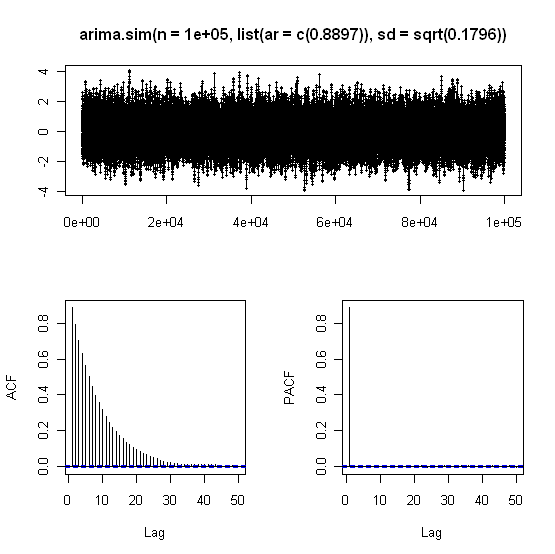
\includegraphics[width=.8\linewidth]{ SimAR1.png}
\caption{Simulation of AR(1) : >\texttt{tsdisplay(arima.sim(n=100000,list(ar = c(0.8897)),sd = sqrt(0.1796)))}}
\label{fig:sim1}
\end{center}
\end{figure}

\begin{figure}[!h]
\begin{center}
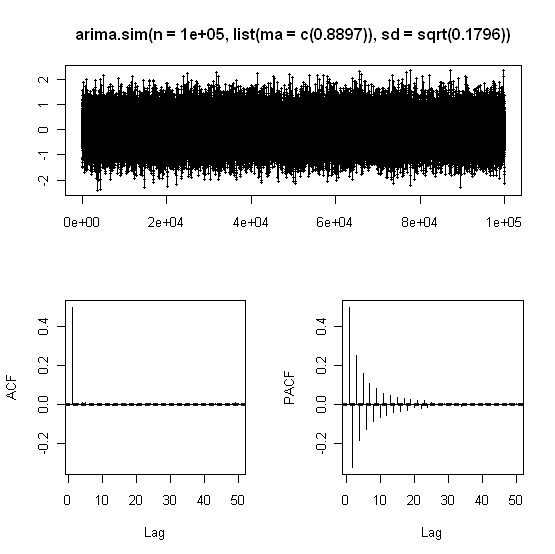
\includegraphics[width=.8\linewidth]{ SimMA1.png}
\caption{Simulation of MA(1) : >\texttt{tsdisplay(arima.sim(n=100000,list(ma = c(0.8897)),sd = sqrt(0.1796)))}}
\label{fig:sim2}
\end{center}
\end{figure}

\begin{figure}[!h]
\begin{center}
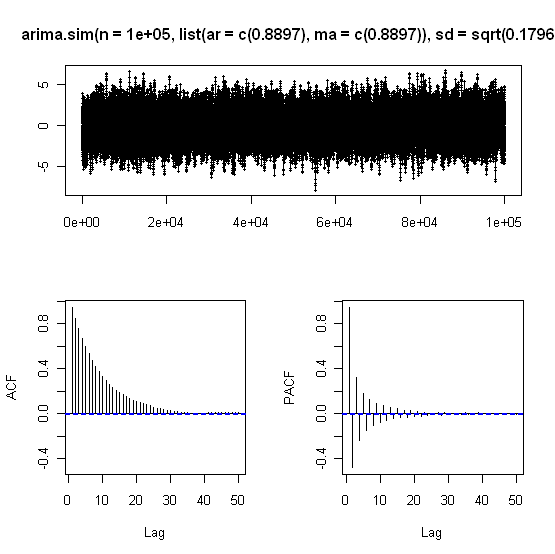
\includegraphics[width=.8\linewidth]{ SimAR1MA1.png}
\caption{Simulation of ARMA(1,1) : >\texttt{tsdisplay(arima.sim(n=100000,list(ar=c(.8897),ma = c(0.8897)),sd = sqrt(0.1796)))
}}
\label{fig:sim3}
\end{center}
\end{figure}


\section{Stationarity in mean and variance}

\begin{definition}[Stationary in mean]
A time series is called {\it stationary in mean} if it randomly
fluctuates about a {\it constant} mean level. 
\end{definition}


\noindent EXERCISE: 
\begin{enumerate}
\item Are the simulated times series in figures \ref{fig:sim1}, \ref{fig:sim2} and \ref{fig:sim3}  stationary in mean?
\item what types of patterns of a time series would
imply  that it is not stationary in mean?
\end{enumerate}

Stationary series are `nice' because they are not complicated.
They are easily modelled and fitted (an ARMA model will
usually do) and we do not have to worry about seasonal or
trend/cycle.

\vspace{.2cm}

In fact, in time series modelling, the term \emph{stationarity} has a more general meaning. There are three key parts that make a series stationary:
\begin{itemize}
\item The mean is constant (stationary in mean)
\item The variance is finite (stationary in variance)
\item The correlation between values in the time series depends \emph{only} on
the time distance between these values. (stationary in autocorrelation)
\end{itemize}
We spend most of our time discussing the first two.



\begin{definition}[Stationarity in variance]
 In addition to stationarity
in mean, a time series is said to be {\it stationary in variance} if
the variance in the time series does not change with time. 
\end{definition}

\noindent EXERCISE: 
\begin{enumerate}
\item Are the simulated times series in figures \ref{fig:sim1}, \ref{fig:sim2} and \ref{fig:sim3}  stationary in variance?

\item As well as non-stationarity in both mean and
variance, series can also be: non-stationary in mean and stationary
in variance; or stationary in mean and non-stationary in variance;
or non-stationary in both. Sketch time series with each of
these three properties. 

\end{enumerate}


\section{Conclusion}

ARMA models are not able to handle time series that are not stationary in mean and variance.
In other word, ARMA models should only be fitted to time series that are stationary in mean (i.e. no trend or no seasonal pattern)
and stationary in variance.
 



%%%%%%%%%%%%%%%%%%%%
\chapter{ Using ACF and PACF to select  MA(q) or AR(p) models}
\label{chp:ACF:PACF:AR:MA}
 

The principle way to
determine which AR or MA model is appropriate is to look at the ACF
and PACF of the time series. The table \ref{tab:ACF:PACF:AR:MA} gives the theoretical
behaviour of these functions for different MA and AR models. An
informal way to pick a model is to compute the ACF and PACF for a
time series and match it to the behaviour in the table \ref{tab:ACF:PACF:AR:MA}.
This rule is however difficult to use when the time series is explained by an ARMA model (combined effect of AR and MA).



\vspace{.2cm}

\begin{table}[!h]
\begin{center}
\begin{tabular}{lp{6.5cm}p{6.5cm}} \hline
{\bf MODEL} & {\bf ACF} & {\bf PACF} \\[.2cm] \hline
AR(1) & Exponential decay: on +ve side if $\phi_1>0$ and alternating
in sign, starting on $-$ve side, if $\phi_1<0$. & Spike at lag 1,
then 0; +ve
spike if $\phi_1>0$ and $-$ve spike if $\phi_1<0$. \\
AR($p$) & Exponential decay or damped sine wave. The exact pattern
depends on the signs and sizes of $\phi_1,\ldots,\phi_p$. & Spikes
at lags 1 to $p$, then zero. \\
MA(1) & Spike at lag 1, then 0; +ve spike if $\psi_1<0$ and $-$ve
spike if $\psi_1>0$. & Exponential decay: on +ve side if $\psi_1<0$
and alternating in sign, starting on +ve side, if
$\phi_1<0$. \\
MA($q$) & Spikes at lags 1 to $q$, then zero. & Exponential decay or
damped sine wave. The exact pattern depends on the signs and sizes
of $\psi_1,\ldots,\psi_q$. \\ \hline
\end{tabular}
\end{center}
\caption{Shapes of ACF and PACF to identify AR or MA models suitable to fit time series.}\label{tab:ACF:PACF:AR:MA}
\end{table}


\section{ACF and PACF}

\begin{definition}[ACF]
At lag $k$, the ACF is computed by:
$$
ACF(k)=\frac{\mathbb{E}\left\lbrack \left(y_t-\mathbb{E}[y_t]\right) \left(y_{t-k}-\mathbb{E}[y_{t-k}]\right) \right\rbrack}{\sqrt{\mathbb{V}ar[y_t]\mathbb{V}ar[y_{t-k}]}}
$$
\end{definition}


In time series, we may want to measure the
relationship between $Y_t$ and $Y_{t-k}$ when the effects of other
time lags $1,2,\ldots,k-1$ have been removed. The autocorrelation
does not measure this. However, {\it Partial autocorrelation} is a
way to measure this effect.

\begin{definition}[PACF]
The partial autocorrelation of a time series at lag $k$ is denoted
$\alpha_k$ and is found as follows:
\begin{enumerate}
\item Fit a linear regression of $y_t$ to the first $k$ lags (i.e.\ fit
an AR($k$) model to the time series):
\[ y_t = \phi_0 + \phi_1 y_{t-1} + \phi_2 y_{t-2} + \cdots + \phi_k
y_{t-k} +\epsilon_t \]
\item Then $\alpha_k = \hat{\phi}_k$, the fitted value of $\phi_k$ from
the regression (Least Squares).
\end{enumerate}
The set of partial autocorrelations at different lags is called the
{\it partial autocorrelation function} (PACF) and is plotted like
the ACF. 
\end{definition}


%%

\section{Exercises:  ACF and PACF for AR(1) and MA(1)}



\begin{enumerate}

\item Assuming AR(1) model with $\phi_0=0$, show that the PACF coefficients are zeros when $k>1$.\\
\vspace{.3cm}

\textbf{Ans.}\textit{
By definition, the model is (ignoring the constant term $\phi_0$) :
$$
y_t=\phi_1\ y_{t-1}+\epsilon_t
$$
Computing the PACF at order 2 for instance, implies to fit a AR(2) model to our AR(1).
This is easily done: 
$$
y_t=\phi_1\ y_{t-1}+0\ y_{t-2}+\epsilon_t
$$
therefore the PACF coefficient at lag 2, is 0.
The same reasoning can be used for any $k>1$.
At lag $k=1$, the PACF coefficient is $\phi_1$.
This explains the  shape of the PACF you have for a simulated AR(1) model using R.
}
\vspace{.3cm}



\item Lets assume a  MA(1) model with $\psi_0=0$
\begin{enumerate}
\item what is $\mathbb{E}[y_t]$?\\
\textbf{Ans.}\textit{
$$
\begin{array}{ll}
\mathbb{E}[y_t]&=\mathbb{E}[\psi_1\ \epsilon_{t-1}+\epsilon_t] \quad\text{By def. of our MA(1)}\\
&=\psi_1\ \mathbb{E}[\epsilon_{t-1}]+\mathbb{E}[\epsilon_t] \quad\text{Expectation is a linear operator}\\
&=\psi_1\ 0+0 \quad\text{Since }\epsilon_t\sim\mathcal{N}(0,\sigma^2)\ \forall t \text{(i.e. expectation of the errors is 0)}\\
&=0\\
\end{array}
$$
}
\item What is the variance of $y_t$?\\
\textbf{Ans.}\textit{
$$
\begin{array}{ll}
\mathbb{V}ar[y_t]&=\mathbb{E}[(y_t-\mathbb{E}[y_t])^2] \quad\text{By def. of variance}\\
&=\mathbb{E}[(y_t)^2] \quad\text{since}\ \mathbb{E}[y_t]=0\\
&=\mathbb{E}[(\psi_1\ \epsilon_{t-1}+\epsilon_t)^2] \quad\text{By def. of our MA(1)}\\
&=\mathbb{E}[\psi_1^2\ \epsilon_{t-1}^2+\epsilon_t^2+2\psi_1\ \epsilon_{t-1}\epsilon_t] \\
&=\psi_1^2\ \mathbb{E}[\epsilon_{t-1}^2]+\mathbb{E}[\epsilon_t^2]+2\psi_1\ \mathbb{E}[\epsilon_{t-1}\epsilon_t] \\
&=\psi_1^2\ \sigma^2+\sigma^2+2\psi_1\ 0 \quad\text{Using the  hypothesis on the errors}\\
\end{array}
$$
Remember that all errors $\epsilon$ follow a Normal distribution with mean 0 ($\mathbb{E}[\epsilon_{t}]=0,\ \forall t$), and variance $\sigma^2$. In addition, the errors are independent from each other i.e.:
$$
\mathbb{E}[\epsilon_{t_1}\epsilon_{t_2}]=0\quad  \forall t_1\neq t_2
$$
}
\item What is the covariance of $y_t$ and $y_{t-k}$?\\
\textbf{Ans.}\textit{
$$
\begin{array}{ll}
\mathbb{C}ov[y_t,y_{t-k}]&=\mathbb{E}[(y_t-\mathbb{E}[y_t])(y_{t-k}-\mathbb{E}[y_{t-k}])] \quad\text{By def. of covariance}\\
&=\mathbb{E}[(y_t)(y_{t-k})] \quad\text{Because }\mathbb{E}[y_t]=0\quad \forall t\\
&=\mathbb{E}[(\psi_1 \epsilon_{t-1}+\epsilon_t)(\psi_1 \epsilon_{t-1-k}+\epsilon_{t-k})] \quad\text{Because of our MA(1) model}\\
&=\mathbb{E}[\psi_1^2 \epsilon_{t-1-k} \epsilon_{t-1}+\psi_1 \epsilon_{t-1-k} \epsilon_{t}+\psi_1  \epsilon_t\epsilon_{t-1-k}\epsilon_t+\epsilon_{t-1}\epsilon_{t-k})] \\
&=\psi_1^2 \underbrace{\mathbb{E}[ \epsilon_{t-1-k} \epsilon_{t-1}]}_{=0, \forall k\geq1}+\psi_1 \underbrace{\mathbb{E}[ \epsilon_{t-k} \epsilon_{t-1}]}_{0, \forall k>1;\  \sigma^2 for k=1}+
\psi_1 \underbrace{\mathbb{E}[  \epsilon_t\epsilon_{t-1-k}]}_{0, \forall k}+\underbrace{\mathbb{E}[ \epsilon_{t}\epsilon_{t-k})] }_{0, \forall k>0}\\
\end{array}
$$
so  $\mathbb{C}ov[y_t,y_{t}]=(\psi_1^2+1) \sigma^2$, $\mathbb{C}ov[y_t,y_{t-1}]=\psi_1 \sigma^2$ and $\mathbb{C}ov[y_t,y_{t-k}]=0, \ \forall k>1$. 
}

\item What is the correlation of $y_t$ and $y_{t-k}$? \\
\vspace{.3cm}

\textbf{Ans.}\textit{ The correlation is the covariance divided by the variances:
$$
\mathbb{C}orr[y_t,y_{t-k}]=\frac{\mathbb{C}ov[y_t,y_{t-k}]}{\sqrt{\mathbb{V}ar[y_t] \mathbb{V}ar[y_{t-k}]}}=
\left\lbrace\begin{array}{l} 
1\quad \text{if  } k=0 \\
\frac{\psi_1}{\psi^2_1+1}\quad \text{if  } k=1 \\
0\quad \text{otherwise } t>1\\
\end{array}
\right.
$$
}

\end{enumerate}
\item Conclude about the form of the ACF function for a MA(1) models? \\
\vspace{.3cm}

\textbf{Ans.}\textit{ 
The ACF plots the lags $k$ on the x-axis, and the y-axis reports the correlation
$\mathbb{C}orr[y_t,y_{t-k}]$.
}

\end{enumerate}


\section{Least Squares algorithm for MA models ?}
Consider an MA(1) (with $\psi_0=0$ for simplification)
$$
y_t=\psi_1 \ \epsilon_{t-1}+\epsilon_t
$$
we need to write this with lagged series of $y_t$ (for which we have the observations $y_1,\cdots,y_n$).
The model can be rewritten:
$$
\begin{array}{ll}
y_t &=\psi_1\ y_{t-1}-\psi_1^2\ \epsilon_{t-2} +\epsilon_t \\
 &=\psi_1\ y_{t-1}-\psi_1^2\ y_{t-2} +\psi_1^3\ \epsilon_{t-3} +\epsilon_t \\
\vdots&\\
y_t &=\psi_1\ y_{t-1}-\psi_1^2\ y_{t-2} +\cdots+(-1)^{t}\psi_1^{t-1}\ y_{1}+\psi_1^t\ \epsilon_{0}+\epsilon_t \\
\end{array}
$$
Assuming $\epsilon_0=0$, $y_t$ is a weighted average of all the past observations, and the expression is not linear w.r.t. the parameter to estimate $\psi_1$ (powers of $\psi_1$ appear in the equation). Hence the Least square algorithm used for estimation with AR models cannot be used.




%%%%%%%%%%%%

\chapter{The backshift operator}
\label{chp:backshift}

\section{Definition}
\begin{definition}[Backshift operator]
In what follows, it will be very useful to denote a lagged series by
using the {\it backshift operator} $B$:
\[ By_t = y_{t-1}, \]
For lags of length $k$, we apply $B$ $k$ times:
\[ y_{t-2} = By_{t-1} = B(B y_t) = B^2 y_t ; \;\; \mbox{in general } B^k y_t = y_{t-k}. \]
\end{definition}
We can use $B$ to express differencing:
\[ y^{\prime}_t = y_t - y_{t-1} = y_t - By_t = (1-B)y_t. \]
The great power of the backshift operator is that it is {\it
multiplicative}: 
\[ (1-B)(1-B^s)y_t = (1 - B - B^s + B^{s+1})y_t = y_t - y_{t-1} - y_{t-2} + y_{t-s-1}, \]




\section{Exercises.}
\begin{enumerate}
\item  Write an MA(1) model with the backshif operator
\item  Write an AR(1) model with the backshif operator
\item  Write an MA(q) model with the backshif operator
\item  Write an AR(p) model with the backshif operator
\item Write an ARMA(p,q) model with the backshif operator



\end{enumerate}


%%%%%%%%%%%%%%%%%%%%%%%%%

\chapter{AIC and BIC}

\label{chp:AIC:BIC}


In the lab, we have tried to find the best ARMA models by using the ACF and PACF graphs to identify the AR(p) and MA(q) components.
Several ARMA(p,q) were then tested until all ACF and PACF coefficients becomes negligeable, and also when the time plot of the residuals looks like noise.

One way to allow you to choose any ARMA model is simply to consider
a lot of different ARMA models, fit them, and choose the one that
has the smallest mean square error (as we have done before when
picking the best parameter value in exponential smoothing, etc.)
There is a problem with this though; we can always make the MSE
smaller by adding another MA or AR term! So if we did this, then we
would just keep finding more and more complicated models that fit
better and better!

Clearly, what we want is a compromise between a model that fits well
but does not have too many parameters. There is no one way to do
this, but one technique is to use {\it information
criterion}.

\section{Information Criterion}

\begin{definition}[AIC and BIC criteria]
 We define two types of information criterion: the \textit{Bayesian Information Criterion} (BIC) and the \textit{Akaike Information Criterion} (AIC). In AIC and BIC, we choose the model that has the minimum
value of:
\[ AIC = - 2 \log(L) + 2m, \]
\[ BIC = - 2 \log(L) + m \log n, \]
where
\begin{itemize}
\item $L$ is the likelihood of the data with a certain model, 
\item $n$ is the number of observations and
\item $m$ is the number of parameters in the model. The number of parameters is $m=p+q$ for an ARMA(p,q) model. % that is $m = p+q+P+Q$.
\end{itemize}
\end{definition}

We see that as the model gets more complicated, the model will fit
better, and $-2 \log(L)$ gets smaller, but $m$ gets bigger. The best
model will be the one that achieves a compromise between the two.
Finally, often the likelihood is difficult to calculate, but there
is a useful approximation:
\[ - 2 \log(L) \approx n (1 + \log(2 \pi)) + n \log (s^2), \]
where $n$ is the number of observations in the series and $s^2$ is
the estimated variance of the residuals after fitting the model. Therefore we
find the model where
\[ \text{AIC} \approx n (1 + \log(2 \pi)) + n \log (s^2) + 2m \] is the smallest.
Again, a forecasting computer package will allow you to hunt for the
ARMA model with the smallest AIC or BIC.

%%%%%%%%%%%%%%
\section{R output}
Tables \ref{tab:AR1:ARMA} and \ref{tab:AR1:ARMA}  show the R outputs when fitting a AR(1) and AR(2) to the dowjones data.


\begin{table}[!h]
\begin{center}
\begin{tabular}{|p{\linewidth}|}
\hline
\begin{verbatim}
Series: dowjones 
ARIMA(1,0,0) with non-zero mean 

Call: arima(x = dowjones, order = c(1, 0, 0)) 

Coefficients:
         ar1  intercept
      0.9964   116.0329
s.e.  0.0045     4.8878

sigma^2 estimated as 0.1974:  log likelihood = -49.86
AIC = 105.72   AICc = 106.04   BIC = 112.79
\end{verbatim}\\
\hline
\end{tabular}
\caption{Output in R of \texttt{arima(dowjones,order=c(1,0,0))}. }
\label{tab:AR1:ARMA}
\end{center}
\end{table}
\begin{table}[!h]
\begin{center}
\begin{tabular}{|p{\linewidth}|}
\hline
\begin{verbatim}
Series: dowjones 
ARIMA(2,0,0) with non-zero mean 

Call: arima(x = dowjones, order = c(2, 0, 0)) 

Coefficients:
         ar1      ar2  intercept
      1.4990  -0.5049   115.7854
s.e.  0.0993   0.1000     4.1654

sigma^2 estimated as 0.1483:  log likelihood = -38.96
AIC = 85.91   AICc = 86.46   BIC = 95.34
\end{verbatim}\\
\hline
\end{tabular}
\caption{Output in R of \texttt{arima(dowjones,order=c(2,0,0))}. }
\label{tab:AR2:ARMA}
\end{center}
\end{table}


Understanding the R outputs:
\begin{enumerate}
\item what are the coefficients ar1 (and ar2) ? what is the intercept?
\item Write down the mathematical equation of the models fitted in both cases.
\item  What is  sigma?
\item What is log likelihood?
\end{enumerate}
Note that the AIC and BIC are given.




%%%%%%%%%%%%%%%%%%%%%%%%%
\chapter{ARIMA$(p,d,q)$}
\label{chp:ARIMA}


An ARMA model is not suitable for fitting  a times with a trend: 
Remember a time series showing a trend is not stationary in mean and ARMA models are only suited for time series stationary in mean and variance.
Differencing is an operation that can be applied to a time series to remove  a trend. If after differencing the time series looks stationary in mean and variance, then an ARMA(p,q) model can be used.  
Section \ref{sec:differencing} presents differencing (of order $d$) and section \ref{sec:ARIMA} extends the ARMA(p,q) models to the ARIMA(p,d,q) models. 

%%%%
\section{Differencing a time series}
\label{sec:differencing}

Consider a time series $y_t$, the first order differencing is defined as 
$$
y^{\prime}_t = y_t - y_{t-1}
$$
We can use $B$ to express differencing:
\[ y^{\prime}_t = y_t - y_{t-1} = y_t - By_t = (1-B)y_t. \]

\paragraph{Exercise.} Express the second order difference
$y^{\prime\prime}_t = y^{\prime}_t - y^{\prime}_{t-1}$ in terms of the backshift operator
$B$. Conclude on the differencing of order $d$.

\paragraph{Visualisation.}
Figures  \ref{fig:diff:dowjones}, \ref{fig:diff:dowjones:d1} and \ref{fig:diff:dowjones:d2} shows the dowjones time series before and after differencing with $d=1$ and $d=2$. 
\begin{figure}[!h]
\begin{center}
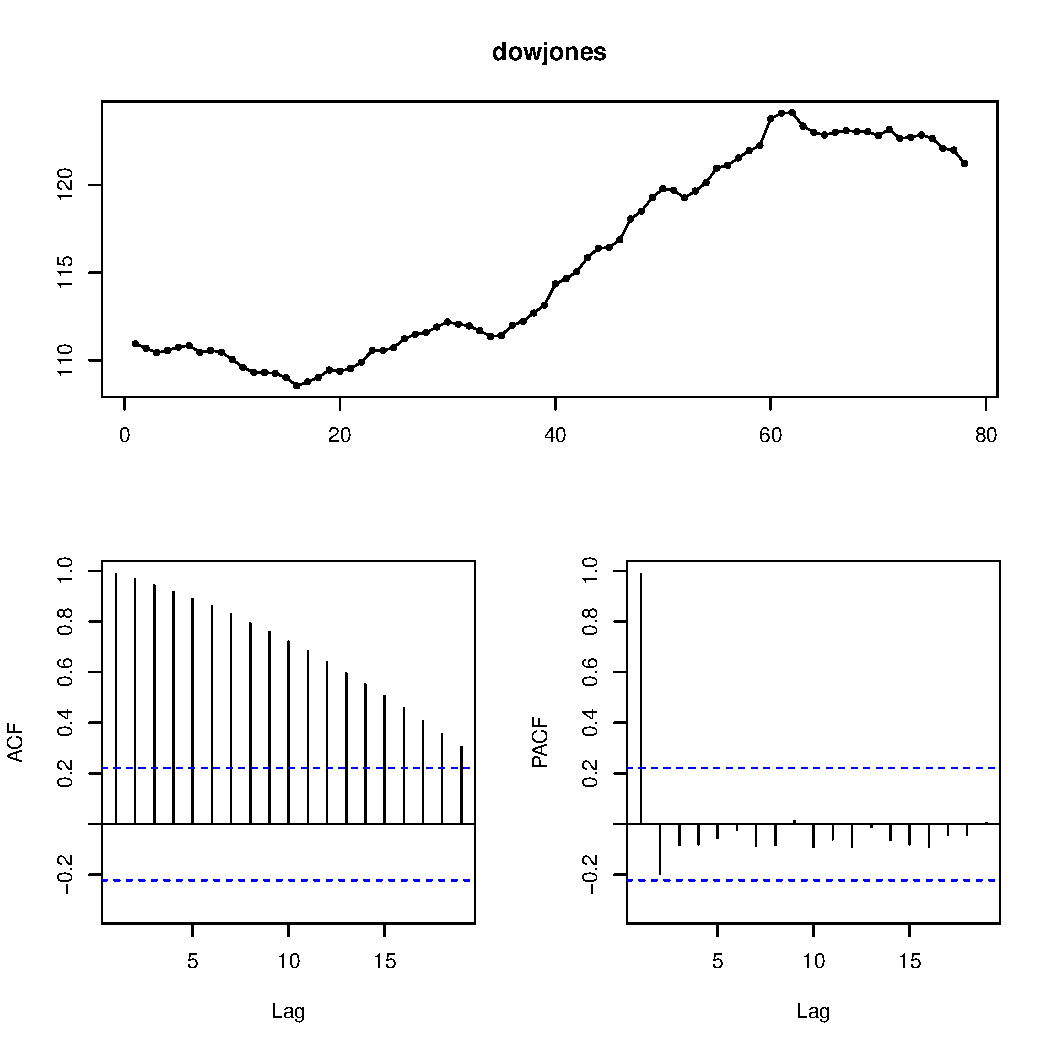
\includegraphics[width=.5\linewidth]{ dowjones.pdf}
\caption{Dowjones time series. \texttt{>tsdisplay(dowjones)}}\label{fig:diff:dowjones}
\end{center}
\end{figure}


\begin{figure}[!h]
\begin{center}
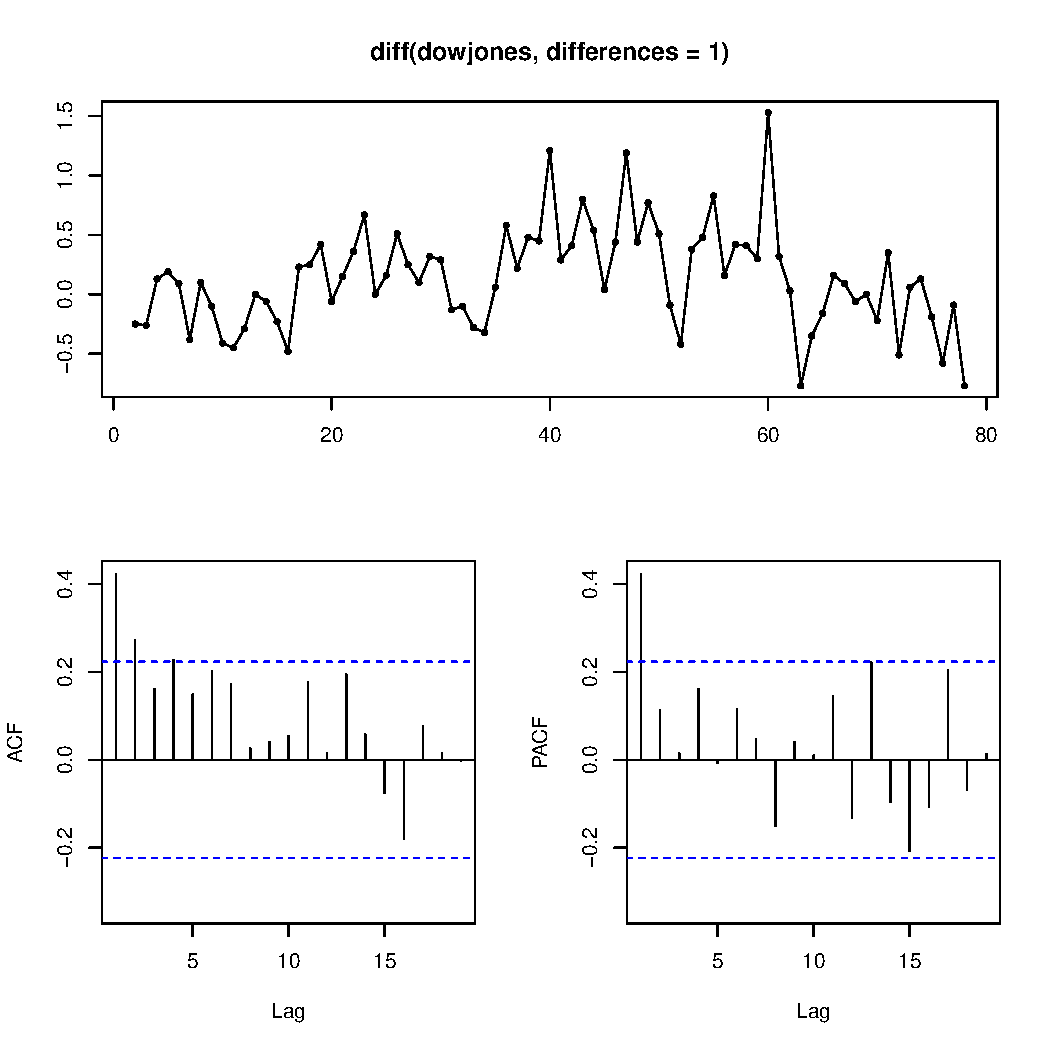
\includegraphics[width=.5\linewidth]{ dowjonesd1.pdf}
\caption{Differencing of the Dowjones time series $d=1$. \texttt{>tsdisplay(diff(dowjones,differences=1))}}\label{fig:diff:dowjones:d1}
\end{center}
\end{figure}

\begin{figure}[!h]
\begin{center}
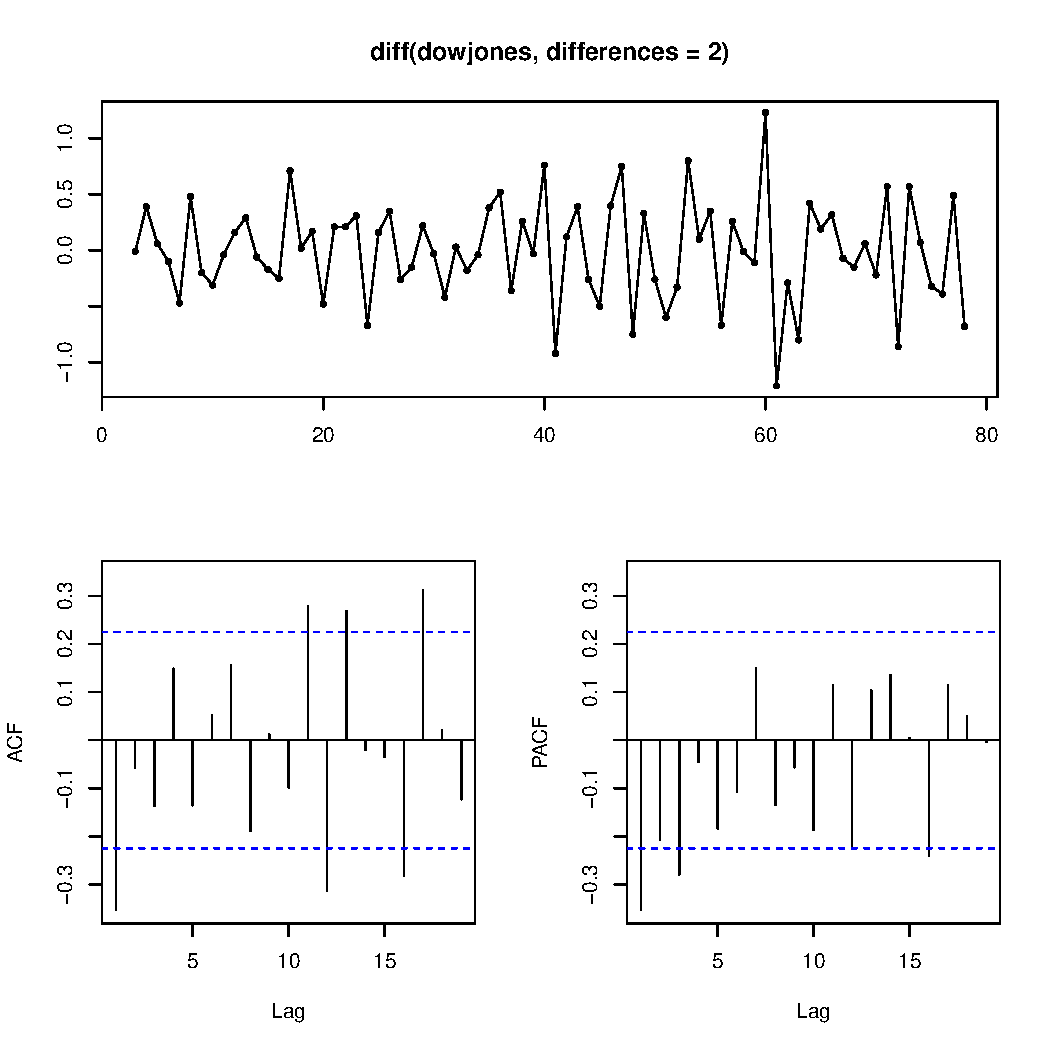
\includegraphics[width=.5\linewidth]{ dowjonesd2.pdf}
\caption{Differencing of the  Dowjones time series $d=2$. \texttt{>tsdisplay(diff(dowjones,differences=2))}}\label{fig:diff:dowjones:d2}
\end{center}
\end{figure}




%%%%
\section{Integrating differencing into ARMA models}
\label{sec:ARIMA}


\begin{definition}[Autoregressive integrated moving average (ARIMA(p,d,q))]
Trends in time series can be  removed by  differencing the time series. This differencing is integrated into
the ARMA models creating the ARIMA models.
ARIMA(p,d,q) define models  with an AutoRegressive part of order $p$, a Moving average part of order $q$ and having applied $d$ order differencing:
$$ 
 \underbrace{(1-\phi_1 B-\phi_2 B^2-\cdots-\phi_{p} B^{p})}_{AR(p)}\ \underbrace{(1-B)^d}_{I(d)}\ y_t =c+ \underbrace{(1-\psi_1 B-\psi_2 B^2-\cdots-\psi_{q} B^{q})}_{MA(q)}\ \epsilon_t
$$

\end{definition}



\paragraph{Example: Random Walk}
The Random walk is an ARIMA(0,1,0):
$$
(1-B)^1 y_t=\epsilon_t
$$
or 
$$
y_t=y_{t-1}+\epsilon_t
$$


\paragraph{Exercises}


\begin{enumerate}



\item  In the table overpage are some data to which we wish to fit the ARIMA(1,1,1) model
$$(1 - 0.4\ B) (1-B)\ y_t = 0.1 + (1-0.9\ B)\ \epsilon_t. $$
If we let $x_t = (1-B)y_t$ be the differenced series, we can fit the simpler ARMA(1,1) model:
$$(1 - 0.4\ B)\ x_t = 0.1 + (1-0.9\ B)\ \epsilon_t. $$
We can re-write this as $x_t= 0.1 + 0.4\ x_{t-1} - 0.9\ \epsilon_{t-1} + \epsilon_t$, and so create fitted values $\hat{x}_t$. With these fitted values we can back transform to get fitted values $\hat{y}_t = \hat{x}_t + y_{t-1}$. Use these facts to fill in the table.

\vspace{.2cm}
\begin{table}[!h]
\begin{center}
\begin{tabular}{cccccc} \hline
& & & & & \\
Time & Data & Differenced data & Fitted values & Error & Fitted values \\
$t$ & $y_t$ & $x_t=y_t-y_{t-1}$ & $\hat{x}_t = 0.1+0.4x_{t-1}-0.9\ \epsilon_{t-1}$ & $\epsilon_t = x_t-\hat{x}_t$ & $\hat{y}_t = \hat{x}_t + y_{t-1}$ \\
& & & & & \\
\hline
& & & & & \\
& & & & & \\
1 & 9.5 & -- & -- & -- & -- \\
& & & & & \\
& & & & & \\
2 & 13.7 & 4.2 & 0 & 4.2 & \\
& & & & & \\
& & & & & \\
3 & 8.7 & -5.0 & & & \\
& & & & & \\
& & & & & \\
4 & 16.1 & 7.4 & & & \\
& & & & & \\
& & & & & \\
5 & 15.3 & -0.8 & & & \\
& & & & & \\
& & & & & \\
6 & 12.2 & -3.1 & & & \\
& & & & & \\
\hline
\end{tabular}
\end{center}
\caption{ARIMA(1,1,1) $(1 - 0.4 B) (1-B) y_t = 0.1 + (1-0.9B) \epsilon_t. $}
\end{table}
\vspace{.2cm}

\item Here is the ARIMA(1,1,1) model:
\[ (1- \phi_1\ B) \ (1-B)\ y_t = c + (1 - \psi_1\ B) \epsilon_t. \]
Expand this equation and apply the backshift operators to get an
equation for $y_t$ in terms of $y_{t-1}$, $y_{t-2}$, $\epsilon_t$ and
$\epsilon_{t-1}$.


\end{enumerate}


\section{Which $ARIMA(p,d,q)$ model do I use?}

There are a very large number of ARIMA models. Which one is
appropriate for a given data set? There are some things to bear in
mind. First, values of $p$, $q$ or $d$ of more than 3 are very
rarely needed. Second, it is often the case that many different
ARIMA models give more or less the same predictions, so there is
some flexibility in the choice of $p$, $d$ and $q$.  The following
approach can be followed:

\begin{enumerate}
\item Plot the data.

\item Look to see if the data is stationary, that is they are scattered randomly about a constant mean level.
Also look at the ACF and PACF (stationarity is implied by the ACF or
PACF dropping quickly to zero).
\item If there is non-stationarity, such as a trend (we're ignoring seasonal behaviour for the moment!), difference the data.
Practically, at most two differences need to be taken to reduce a
series to stationarity. Verify stationarity by plotting the
differenced series and looking at the ACF and PACF.
\item Once stationarity is obtained, look at the ACF and PACF to see if there is any remaining pattern.
Check against the theoretical behaviour of the MA and AR models to
see if they fit. This will give you an ARIMA model with either no MA
or no AR component i.e. ARIMA(0,$d$,$q$) or ARIMA($p$,$d$,0).
\item If there is no clear MA or AR model, an ARMA model will have to be considered. These can in general
not be guessed from the ACF and PACF, other methods are needed,
based on the ideas of minimising Information Criterion (AIC or BIC).
\end{enumerate}



%%%%%%%%%%%%%%%%%%%%%%%%%%%%%%%%%
\chapter{Seasonal   $ARIMA(p,d,q)(P,D,Q)_s$}
\label{chp:Seasonal:ARIMA}



Time series having a trend and/or a seasonal pattern are not stationary in mean.
We extend ARMA(p,q) models in section \ref{sec:ARIMA} to allow removing a trend before fitting an ARMA model.
Section \ref {sec:seasonal:ARIMA} extends further these new models to allow seasonal pattern to be modelled.


\section{Seasonal $ARIMA(p,d,q)(P,D,Q)_s$}
\label{sec:seasonal:ARIMA}
 As things stand, ARIMA models cannot really cope with seasonal
behaviour; we see that, compared to ARMA models, ARIMA(p,d,q) only models time series with trends.
 We will incorporate now seasonal behaviour and present a general definition of the Seasonal ARIMA models.


\begin{definition}[Seasonal Autoregressive integrated moving average : $ARIMA(p,d,q)(P,D,Q)_s$]
Seasonal ARIMA models are defined by 7 parameters  $ARIMA(p,d,q)(P,D,Q)_s$ 
\begin{multline}
 \underbrace{(1-\phi_1 B-\phi_2 B^2-\cdots-\phi_{p} B^{p})}_{AR(p)}\  \underbrace{(1-\beta_1 B^s-\beta_2 B^{2s}-\cdots-\beta_{P} B^{Ps})}_{AR_s(P)}\ \underbrace{(1-B)^d}_{I(d)} \underbrace{(1-B^s)^D}_{I_s(D)}\ y_t  = \\
c+ \underbrace{(1-\psi_1 B-\psi_2 B^2-\cdots-\psi_{q} B^{q})}_{MA(q)}\ \underbrace{(1-\theta_1 B^s-\theta_2 B^{2s}-\cdots-\theta_{Q} B^{Qs})}_{MA_s(Q)}\ \epsilon_t
\end{multline}
where 
\begin{itemize}
\item $AR(p)$ Autoregressive part of order $p$
\item  $MA(q)$ Moving average part of order $q$
\item $I(d)$  differencing of order $d$
\item $AR_s(P)$ Seasonal Autoregressive part of order $P$
\item  $MA_s(Q)$ Seasonal Moving average part of order $Q$
\item $I_s(D)$   seasonal differencing of order $D$
\item $s$  is the period of the seasonal pattern appearing i.e. $s=12$ months in the Australian beer production data.
\end{itemize}
\end{definition}


The idea behind the seasonal ARIMA is to look at what are the best explanatory variables to model a seasonal pattern.
For instance lets consider the Australian beer production that shows a seasonal pattern of period 12 months.
Then to predict the production at time $t$, $y_t$, the explanatory variables to consider are:
$$
y_{t-12},  y_{t-24},\cdots,\text{and /  or } \epsilon_{t-12},\ \epsilon_{t-24}, \cdots
$$  
For seasonal data, it might also 
make sense to take differences between observations at the same
point in the seasonal cycle i.e. for monthly data with annual cycle,
define differences (D=1)
\[ y_t - y_{t-12}. \]
or (D=2)
\[ y_t -2 y_{t-12}+ y_{t-24}.  \]


\section{Using ACF and PACF to identify  seasonal ARIMAs}

You can use ACF and PACF to identify $P$ or $Q$: 
\begin{itemize}
\item For $ARIMA(0,0,0)(P,0,0)_s$, you should see major peaks on the PACF at $s$, $2s$, ....$Ps$. On the ACF, the coefficients at lags $s$, $2s$, ....$Ps$, $(P+1)s$, ... should form an exponential decrease, or a damped sine wave.
See examples figures \ref{fig:sarima:P1} and \ref{fig:sarima:P2}.
\item $ARIMA(0,0,0)(0,0,Q)_s$, you should see major peaks on the ACF at $s$, $2s$, ....$Qs$. On the PACF, the coefficients at lags $s$, $2s$, ....$Qs$, $(Q+1)s$... should form an exponential decrease, or a damped sine wave.
See examples figures \ref{fig:sarima:Q1} and \ref{fig:sarima:Q2}.
\end{itemize}
When trying to identify   $P$ or $Q$, you should ignore the ACP and PACF coefficients other than $s$, $2s$, ....$Ps$,..  or $s$, $2s$, ....$Qs$,....
In other word, look only at the coefficients computed for multiples of $s$.  

\begin{figure}[!h]
\begin{center}
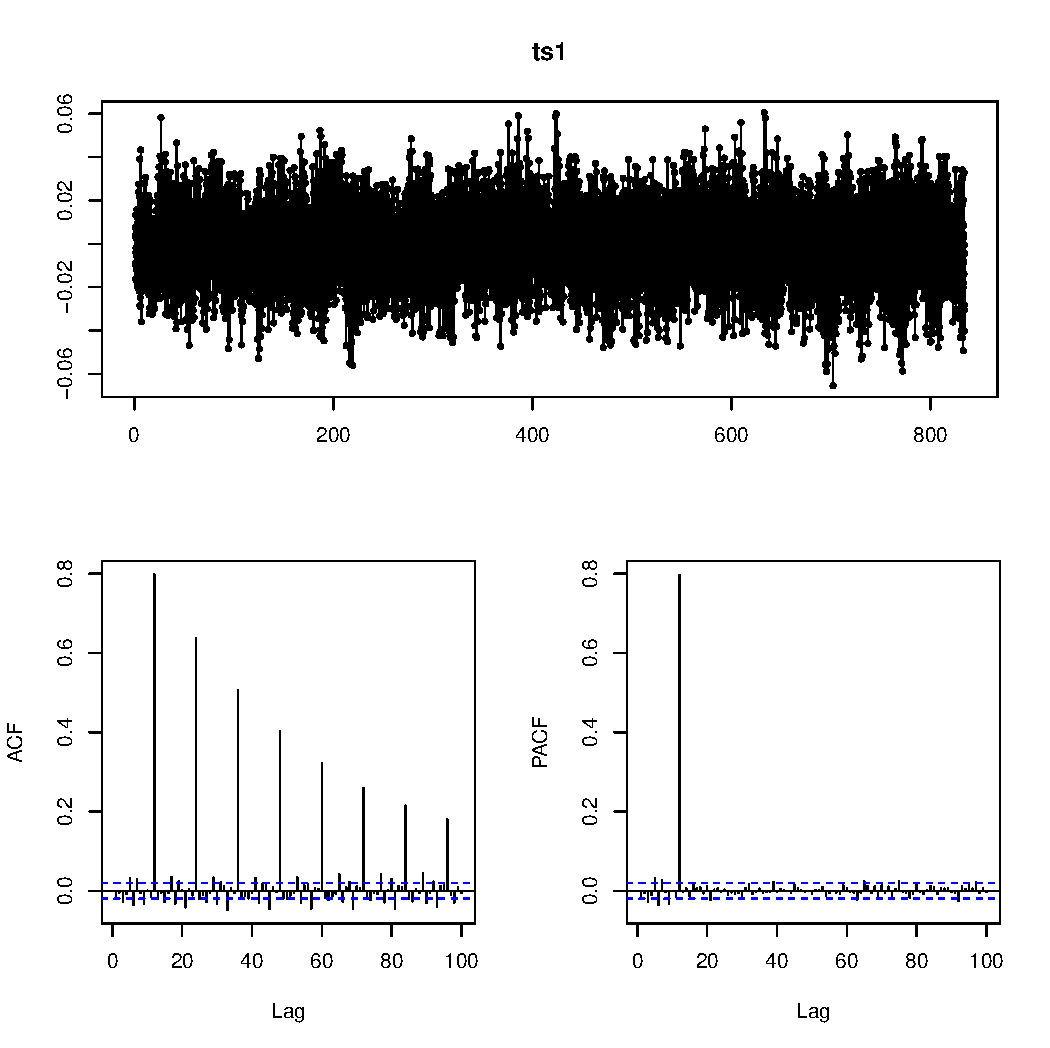
\includegraphics[width=.7\linewidth]{ SARP1.pdf}
\caption{Simulation $ARIMA(0,0,0)(1,0,0)_{12}$}\label{fig:sarima:P1}
\end{center}
\end{figure}

\begin{figure}[!h]
\begin{center}
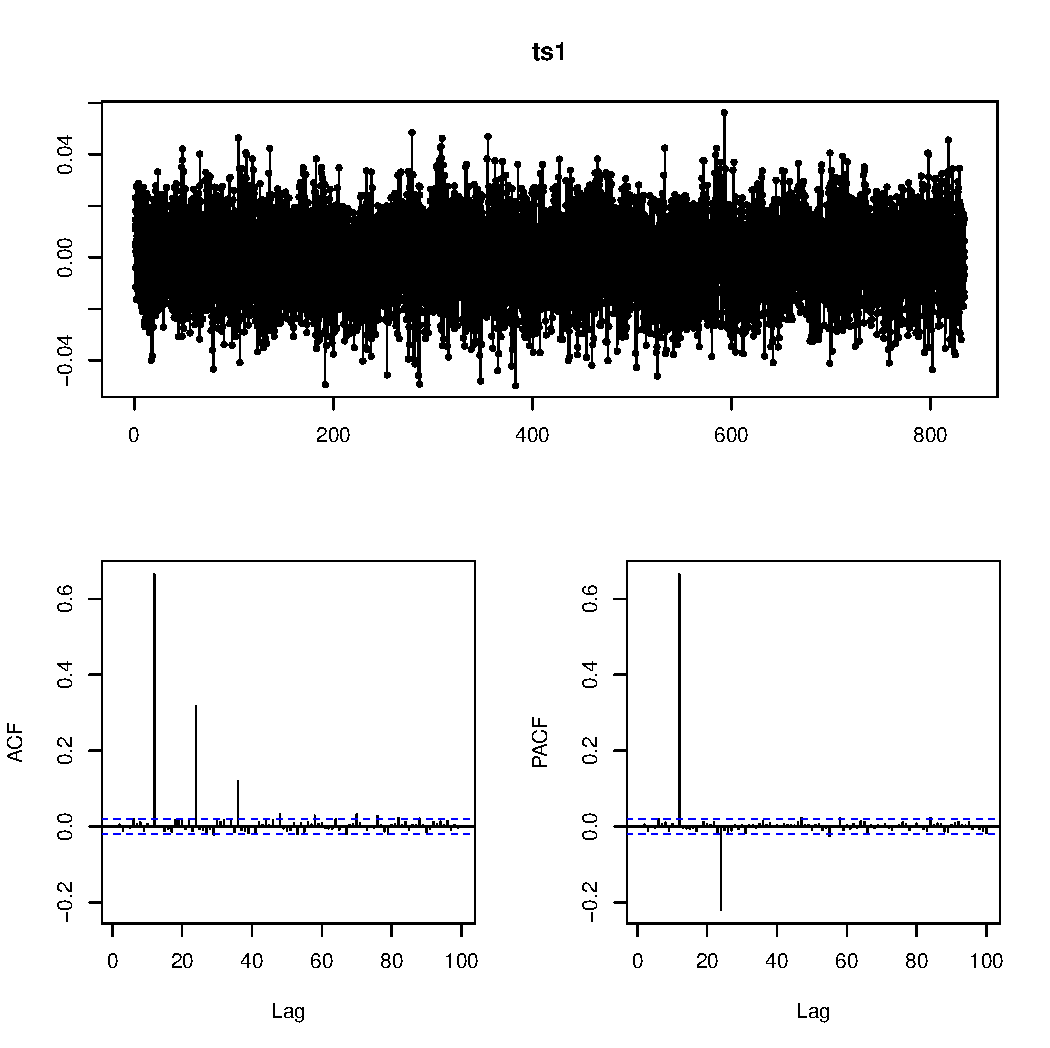
\includegraphics[width=.7\linewidth]{ SARP2.pdf}
\caption{Simulation $ARIMA(0,0,0)(2,0,0)_{12}$}\label{fig:sarima:P2}
\end{center}
\end{figure}

\begin{figure}[!h]
\begin{center}
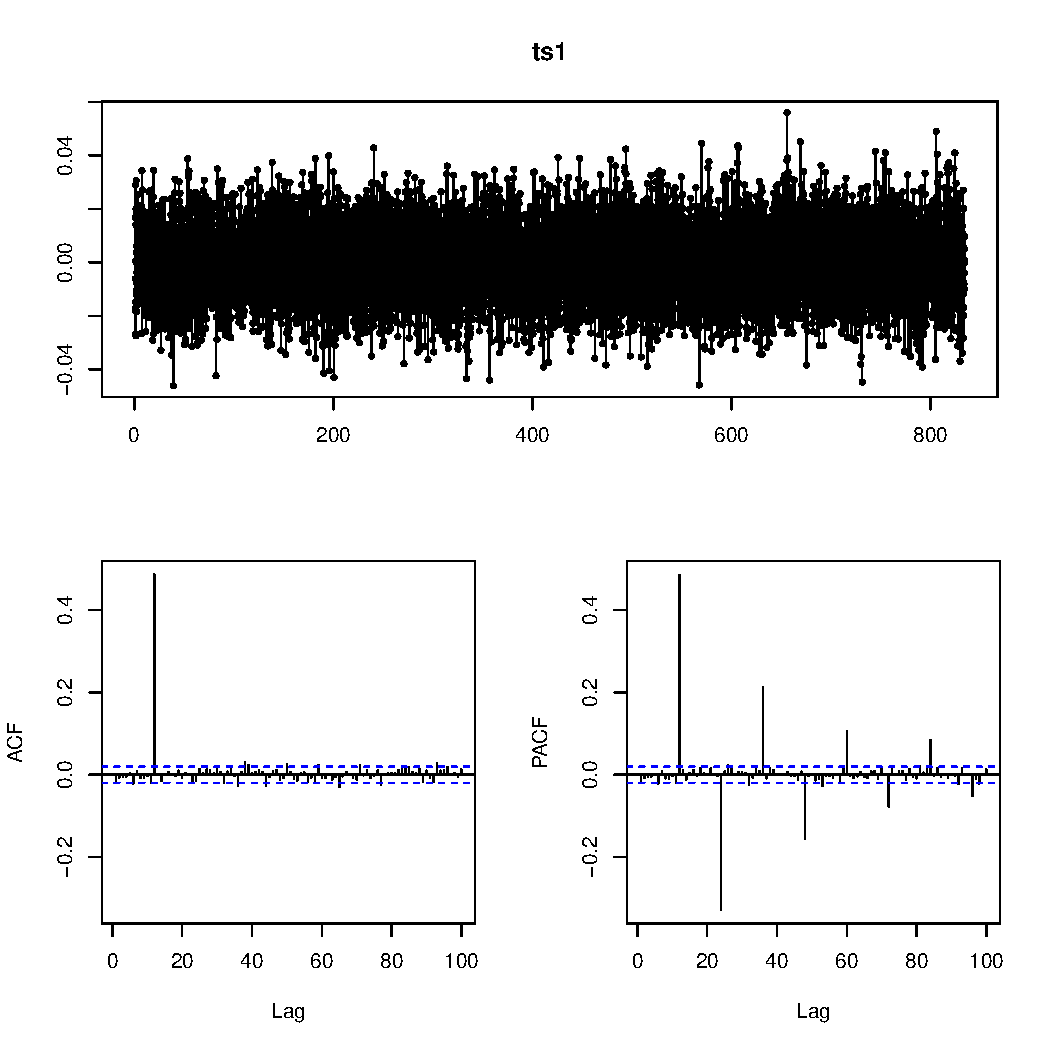
\includegraphics[width=.7\linewidth]{ SMAQ1.pdf}
\caption{Simulation $ARIMA(0,0,0)(0,0,1)_{12}$}\label{fig:sarima:Q1}
\end{center}
\end{figure}

\begin{figure}[!h]
\begin{center}
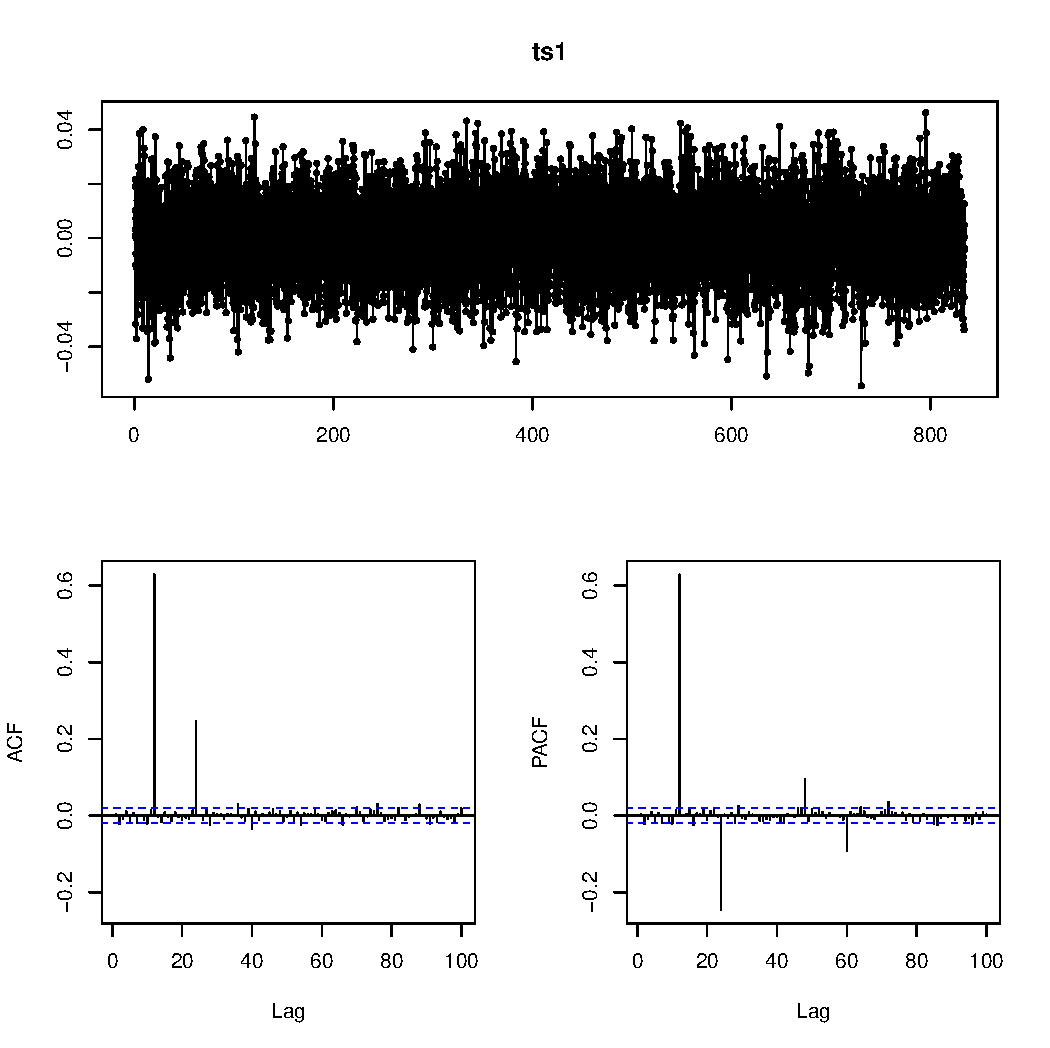
\includegraphics[width=.7\linewidth]{ SMAQ2.pdf}
\caption{Simulation $ARIMA(0,0,0)(0,0,2)_{12}$}\label{fig:sarima:Q2}
\end{center}
\end{figure}

\section{How to select the best Seasonal ARIMA model?}

It is sometimes not possible to identify the parameters p,d,q and P,D,Q using visualisation tools such as ACF and PACF.
Using the BIC as the selection criterion,  we select the ARIMA model with the lowest value of the  BIC.
Using the AIC as the selection criterion, we select the ARIMA model with the lowest value of the  AIC.
 





\section{Conclusion}

We have now defined the full class of statistical models $ARIMA(p,d,q)(P,D,Q)_s$ 
studied in this course. ARMA(p,q) can only be applied to time series stationnary in mean, hence 
the extension to $ARIMA(p,d,q)(P,D,Q)_s$  (introducing $d,D,P,Q,s$) allowed us to make the time series stationary in mean.
Unfortunatly, we still are not able to deal with time series that are not stationary in variance. 
We propose some possible solutions in the next chapter. 
  
  
%%%%%%%%%%%%%%%%%%%%%%%%%%%%%%%%%%%
\chapter{Transforming a time series} 
\label{chp:PreparationTS}


The seasonal arima$(p,d,q)(P,D,Q)$ can only deal with time series that are stationary in variance.
Before using these models, several transformation can make a time series stationary in variance. 

The previous chapters have proposed to make a time series stationary in mean by first removing a trend by differentiation, and second by removing a seasonal pattern by
considering AR and MA models combined with a seasonal differencing.
In this section we focus on making the time series stationary in variance (when needed). 
Observe figure \ref{fig:airpass}. This time series shows both a trend and a seasonal component
therefore it is not stationary in mean.
Note how the amplitude of the seasonal variation increase overtime from year to year: this is an indicator  of a time series that may  not be stationary in variance.



\begin{figure}[!h]
\begin{center}
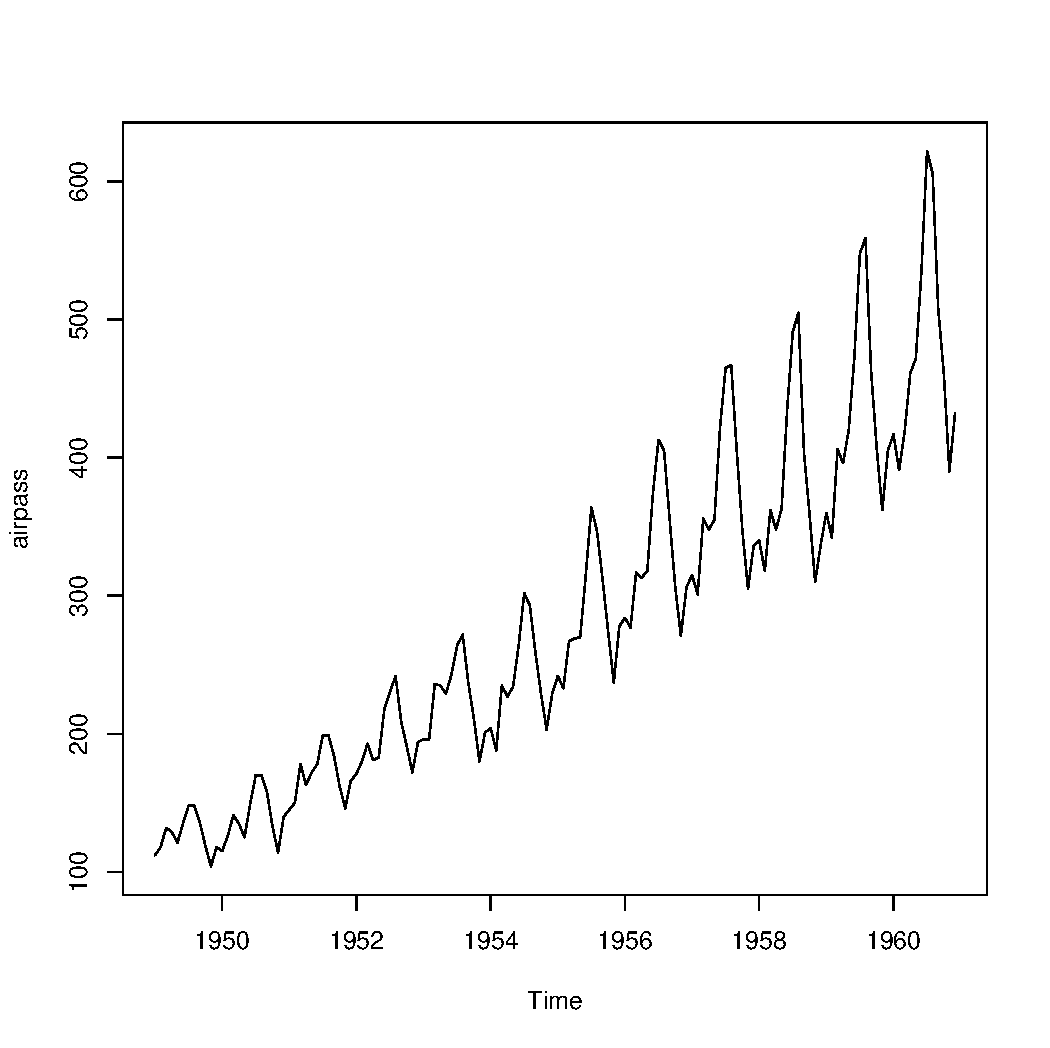
\includegraphics[width=.5\linewidth]{airpass}
\caption{Monthly totals of international airline passengers (1949 to 1960) (time series \texttt{airpass}).}
\label{fig:airpass}
\end{center}
\end{figure}

Mathematical  functions can be applied to the time series to make them stationary in variance.
Four such transformations are commonly used, and reduce variance
by differing amounts. Which one to use depends on how much the
variance is increasing with time.

\vspace{.5cm}

\begin{center}
\begin{tabular}{llc} \hline
Square root & $\sqrt{y_i}$ & $\downarrow$ \\
Cube root   & $\sqrt[3]{y_i}$ & Increasing \\
Logarithm   & $\log(y_i)$ & Strength \\
Negative Reciprocal & $-1/y_i$ & $\downarrow$ \\ \hline
\end{tabular}
\end{center}

\vspace{.5cm}

Square root and logarithm are the most common.

\vspace{.5cm}



\begin{figure}[!h]
\begin{center}
\begin{tabular}{cc}
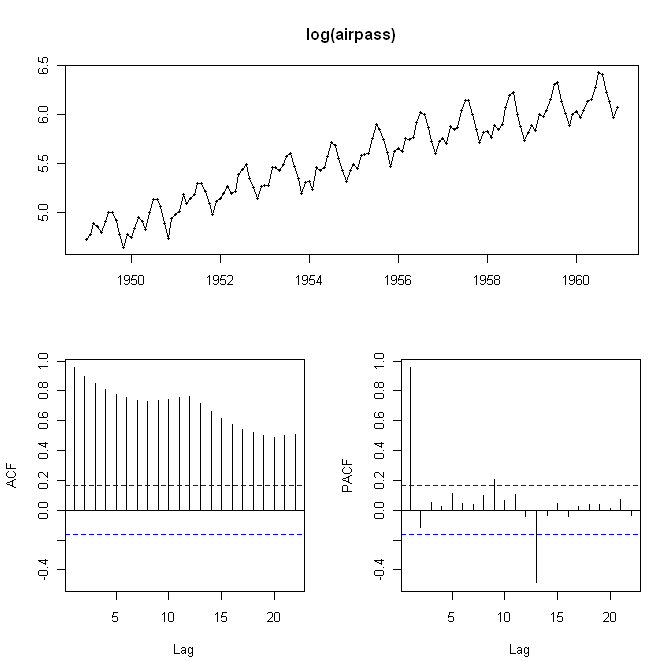
\includegraphics[width=.5\linewidth]{ logairpass.png}&
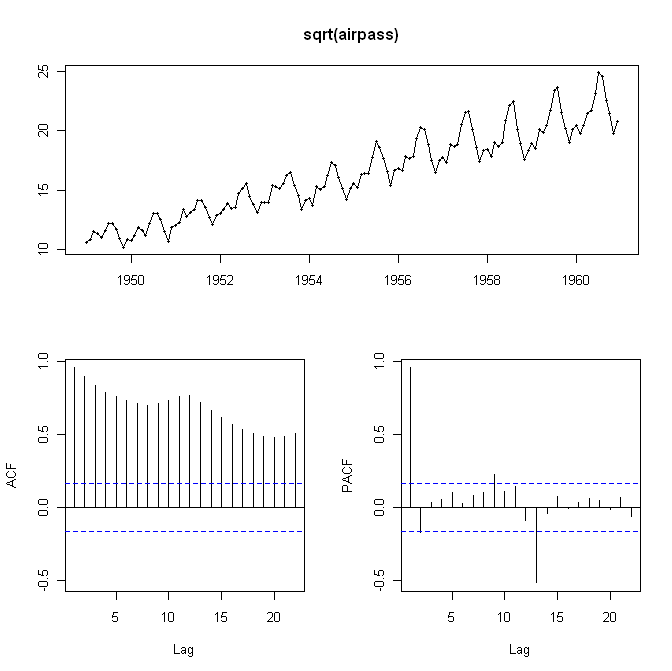
\includegraphics[width=.5\linewidth]{ sqrtairpass.png}\\
 $\log$&$\sqrt{\ }$ \\
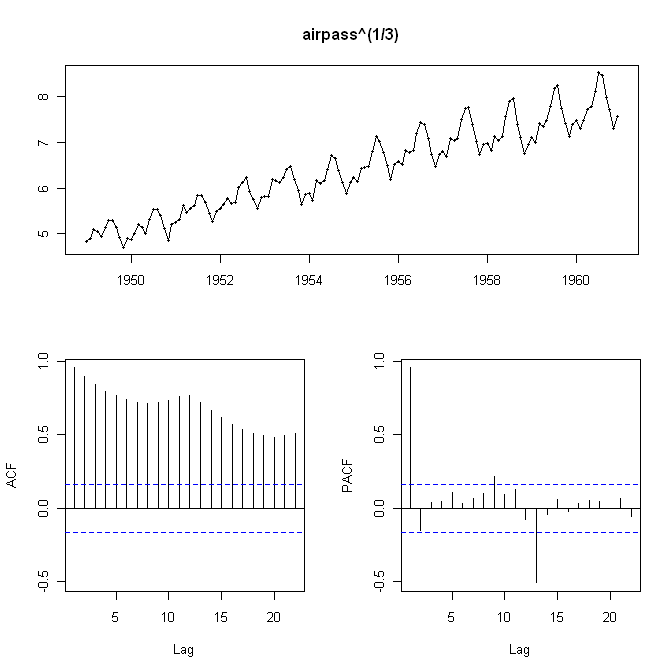
\includegraphics[width=.5\linewidth]{ rootcubeairpass.png}&
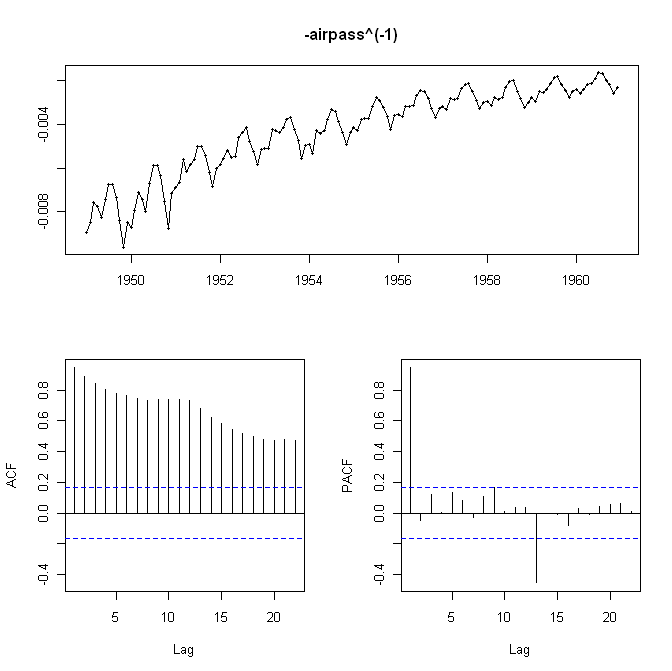
\includegraphics[width=.5\linewidth]{ invairpass.png}\\
 $(\cdot)^{1/3}$&
$-(\cdot)^{-1}$\\
\end{tabular}
\caption{Transformations of \texttt{airpass}.}
\label{fig:airpass:transf}
\end{center}
\end{figure}


\newpage

\noindent\rule[.15 cm]{\linewidth}{.01 cm}

\noindent EXERCISE: look at the four transformations as applied to
the \texttt{airpass} time series (figure \ref{fig:airpass:transf}). Which transformation is best at
stabilising the variance?

\noindent\rule[.15 cm]{\linewidth}{.01 cm}


\paragraph{Final remarks:} It may be difficult to assess non stationarity in variance from the time series itself so an efficient alternative is to fit an ARIMA model (e.g. using \texttt{auto.arima} R function) to the time series and its various transformations,  and visualise in each case the residuals: these should be  having a constant mean 0 and a fixed variance over time when ARIMA is a suited model. 


%%%%%%%%%%%%%%%%%%
%%%%%%%%%%%%%%%%%%
\part{Conclusions}




\chapter{Summary of the course}

We have introduced the Holt-Winters algorithms and the ARIMA models as two classes of techniques to analyse time series. Some Holt-Winters algorithms have an equivalent ARIMA models (cf. table \ref{tab:final}).  Figure \ref{fig:overview} provides a summary to the content of this course. Remember that all these methods rely on the hypothesis that somewhat what has happened in the past repeats itself in the future (continuity hypothesis).

% p.373
\begin{table}[!h]
\begin{center}
\begin{tabular}{lcr}
Simple Exponential Smoothing &$\equiv$& ARIMA(0,1,1)\\
&&\\
\hline
&&\\
Holt's linear method &$\equiv$& ARIMA(0,2,2)\\
&&\\
\hline
&&\\
Holt-Winters' additive method & $\subset$ & ARIMA(0,1,s+1)$(0,1,0)_s$\\
&&\\
\hline
&&\\
Holt-Winters' multiplicative method && no ARIMA equivalent\\
\end{tabular}
\end{center}
\caption{Final remarks about Holt-Winters Algorithms and ARIMA models (\cite{Makridakis} p. 373).}
\label{tab:final}
\end{table}

\begin{figure}[!h]
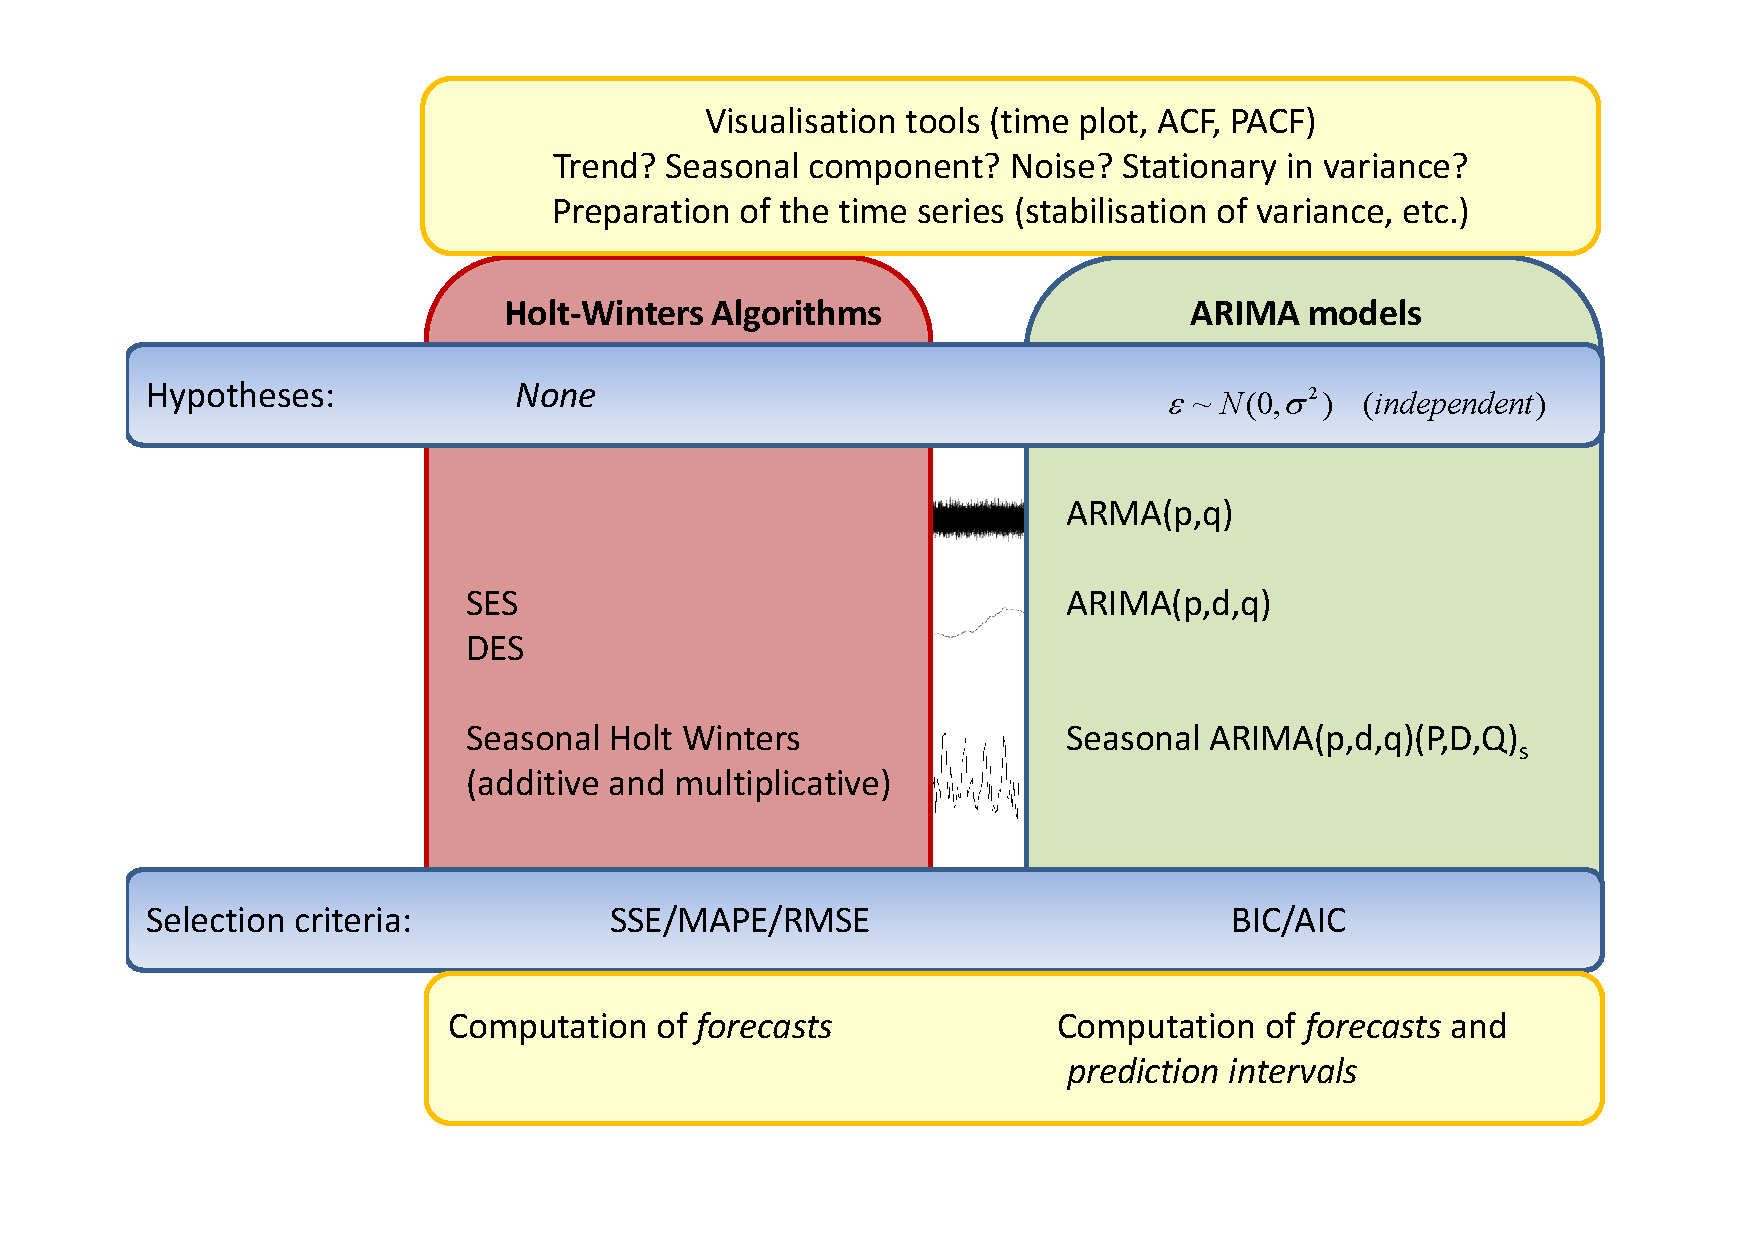
\includegraphics[width=\linewidth]{ForecastingTOC.pdf}
\caption{Course overview.}
\label{fig:overview}
\end{figure}


%%%%%%%%%%%%%%%%%%%%%%%%%%%%%
\chapter{Beyond Holt-Winters algorithms and ARIMA models}




%%%%%%%%%%%%%%%%%%%%
\section{ARCH GARCH}

\label{sec:arch}
In some parts of the course, we have come across series which are non-stationary in variance, and we have transformed the data in some way. These transformations rely on the non-stationarity in variance being highly systematic. For example, in order for the log transformation to work the variability in the data must be increasing as time goes on. It is easy to envisage situations where the variability gets bigger and smaller over time in a non-systematic way. 

\begin{definition}[ARCH]
\textit{Autoregressive Conditional Heteroscedastic (ARCH) models} allow the variance term to have its own random walk, for instance extending AR(1):
\[ y_t = \phi_0 + \phi_1 y_{t-1} + \epsilon_t,\; \; \epsilon_t \sim N(0,\sigma_t^2) \]
so that
\[  \sigma_t^2 = \gamma_0 + \gamma_1\  \sigma_{t-1}^2 \]
\end{definition}
The net effect is to allow the variability in $y_t$ to vary with time; each $y_t$ has its own $\sigma_t$. The parameters $\gamma_0$ and $\gamma_1$ control the amount of variation in $y_t$ at time $t$ by controlling the size of $\sigma_t$.

\begin{definition}[GARCH]
A further generalisation exists, known as \textit{Generalised Autoregressive Conditional Heteroscedastic (GARCH) models}. In this version, the variance terms are given their own ARMA process (rather than the AR process in ARCH models), based on the squares of the error terms. A simple version would now have:
\[ \epsilon_t \sim N(0,\sigma_t^2),\;\; \sigma_t^2 = \gamma_0 + \gamma_1 \sigma_{t-1}^2 + \beta_1 \epsilon_{t-1}^2. \]
where $\epsilon_t$ has the same meaning as in a standard MA process. Further generalisations exist which allow non-linear, non-stationary processes be applied to the variance terms.
\end{definition}


%%%%%%%%%%%%%%%%%%%
\section{Continuous time series modelling}

Here we relax the assumption where $y_t$ can only exist at discrete time points $t=1,2,\ldots,n$. There are many scenarios where we could observe $y$ at irregular time points; we will now write $y(t)$ to describe the measurement of $y$ at a continuous time $t$. Many simple (and, conversely, incredibly complicated) time series models can be written in this format.

\subsection{Brownian motion}

Perhaps the simplest of the continuous time models is that of Brownian motion, also known as a Weiner process. Here we define the differences between data values at different time points to be normally distributed with a very specific mean and autocovariance structure. We can write it as:
\[ y(t) - y(t-s) \sim \mathcal{N}(0,s). \]
Thus the change in value of the series is dependent on the time distance between the values. An obvious extension is:
\[ y(t) - y(t-s) \sim \mathcal{N}(\mu,s \sigma^2), \]
to allow for more complicated variation. In this context the $\mu$ parameter is known as a \textit{drift} parameter as it controls the general direction of the data values as time proceeds.



\subsection{Gaussian processes}

We have already come across one very simple continuous time model in the shape of linear regression. If we let $y(t) = \alpha+\beta t + \epsilon_t$ (so $y_t \sim N(\alpha+\beta t,\sigma^2)$), we already have a technique for determining the value at all times $t$. This is an example of a simple Gaussian process (GP). In general we say that $y(t)$ follows a GP if it has the following properties:
\begin{enumerate}
\item $y(t) \sim \mathcal{N}(\mu(t),\sigma^2 )$,
\item $Cov(y(t),y(t-k)) = f(k) \times \sigma^2$.
\end{enumerate}
Note that this process is not stationary unless $\mu(t)$ is constant. The linear regression example above has $\mu(t)=\alpha+\beta t$ and $f(k)=0$ if $k>0$ and $f(0)=1$. We can build more complicated GPs by allowing a more general structure for $f(k)$; the autocorrelation function. One choice for $f(k)$ is known as the Gaussian autocorrelation function:
\begin{eqnarray*}
f(k) = e^{-\frac{k^2}{h}},
\end{eqnarray*}
where $h$ is a bandwidth term which determines how far apart $y(t)$ and $y(t-k)$ have to be for them still to be correlated. In practice we often write down the the distribution for a GP using a multivariate normal distribution:
\begin{eqnarray*}
\left( \begin{array}{c} y(t_1) \\ y(t_2) \\ \vdots \\ y(t_n) \end{array} \right ) \sim N \left(
\left( \begin{array}{c} \mu(t_1) \\ \mu(t_2) \\ \vdots \\ \mu(t_n) \end{array} \right), \sigma^2
\left( \begin{array}{cccc}
1 & f(t_1-t_2) & \ldots & f(t_n-t_1) \\
f(t_2-t_1) & 1 & & \vdots\\
\vdots & & \ddots & \vdots \\
f(t_1-t_n) & \ldots & \ldots & 1
\end{array} \right)
\right).
\end{eqnarray*}
We still only have a few parameters to estimate. We have those concerning $\mu(t)$ (2 if we use $\mu(t)=\alpha+\beta t$), we have $h$ for the bandwidth, and we have $\sigma^2$. We could again use maximum likelihood to determine these parameters. Furthermore, if we write the model in matrix notation, we have:
\[ \bmat{y} \sim \mathcal{N}(\bmat{\mu},\sigma^2 \bmat{F}). \]
This allows us to use a very handy theoretical result from the normal distribution to predict data at time points we have not observed, $y(t^*)$:
\[ y(t^*)|\bmat{y} \sim \mathcal{N}\left( \mu(t^*)+ \bmat{f}(\bmat{t}-t^*)^T \bmat{F}^{-1} (\bmat{y}-\bmat{\mu}), \sigma^2 \left( 1 - \bmat{f}(\bmat{t}-t^*)^T \bmat{F}^{-1} \bmat{f}(\bmat{t}-t^*) \right) \right). \]
More generally, we can now create predictive distributions for time points other than those observed. Gaussian processes are widely used in practice by Bayesian statisticians as they can be used as prior distributions over random functions.

\section{Fourier analysis for time series}
\label{sec:FT}

A useful way of thinking about time series that have a seasonal component is to use the \textit{frequency} domain rather than the time domain as we have been using. Consider a time series written as:
\[ y_t = a \cos (\omega t) + b \sin( \omega t) + \epsilon_t. \]
We would now have a nice oscillating time series model with the same normally-distributed error, $\epsilon_t$, as before. Indeed, it has been shown that you can write \textit{any} function using this frequency domain approach by adding together lots of different sine and cosine parts (known as harmonics):
\[ y_t = \sum_{j=1}^k a_j \cos( \omega_j t )+ b_j \sin (\omega_j t )+ \epsilon_t. \]
Now we have $k$ harmonics and the series is written as a sum of terms (determining the number of harmonics we require is not always easy). We can adjust the seasonality of the different harmonics by changing the $\omega_j$ terms. For example, if we had daily data with a yearly seasonal trend we could set the first harmonic $\omega_1 = 2 \pi / 365$. We can make the model more complicated by letting the data determine the $\omega$s via, for example, maximum likelihood.



%%%%%%%%%%%%%%%%%%%%
\section{Others techniques used for time series analysis and forecasting}
\begin{itemize}
\item Functional Data Analysis 
\item Neural Networks for time series
\item Kalman Filtering
\item etc.
\end{itemize}


\nocite{}
\bibliographystyle{plain}
\bibliography{Reference370}

\label{mylastpage}


\end{document}
